\documentclass[fr,license=none]{../../../eplsummary}

\usepackage[utf8]{inputenc}
\usepackage{amsmath}
\usepackage{graphicx}
\usepackage{hyperref}
\usepackage{float}
\usepackage{makeidx}
\usepackage{todonotes}

\graphicspath{{img/}}

\hypertitle{Dispositifs Electroniques}{5}{ELEC}{1330}
{Haddou Keil}
{Vincent Bayot et Denis Flandre}

\section{Bandes d'énergie du cristal parfait}
\subsection{Modèle du Cristal}
\subsubsection{Modèle Complet}
Le modèle complet du cristal est composé de $N$ noyaux et $P$ électrons. L'énergie Totale du cristal est donné par l'équation de Schrödinger indépendante du temps (en régime établi).

\begin{gather}
    \mathcal{H}\Phi(\Bar{r_1},...,\Bar{r_p};\Bar{R_1},...,\Bar{R_N}) = E_T\Phi(\Bar{r_1},...,\Bar{r_p};\Bar{R_1},...,\Bar{R_N})\\
    \mathcal{H} = \left[\sum_{j=1}^N\left(\frac{-\hbar^2\nabla_j^2}{2M_j}\right)+\sum_{i=1}^P\left(\frac{-\hbar^2\nabla_j^2}{2M_j}\right)+V(\Bar{r_1},...,\Bar{r_p};\Bar{R_1},...,\Bar{R_N})\right]
\end{gather}
Ici $V$ est le potentiel d'interaction, $R$ et $r$ les positions des noyaux et électrons, et $E_T$ est l'ensemble de l'énergie des noyaux et électrons.
\subsubsection{Approximations}
\textbf{Vibration :} On peut approximer l'énergie de vibration des noyaux et considérer le cristal comme statique, et donc les valeurs $\Bar{R}$ fixes.\\
\textbf{Les électrons de couches profondes sont statiques :} Seuls les électrons quasi-libres et les électrons de valence définissent les propriétés électriques du matériau.\\
\textbf{Il n'y a pas d'interaction entre électrons :} Les électrons ne s'influencent pas les uns les autres.\\
\textbf{Les électrons sont identiques :} Il suffit de construire un seul modèle pour un électron pour représenter le comportement de tous les électrons.
\textbf{L'interaction électron-électron est simplifiée :} On remplace la somme des potentiel d'interaction entre électrons par la valeur moyenne de leur potentiel.
\subsubsection{Modèle de Hartree-Fock}
On ne peut négliger les électrons de valence car ceux-ci contribuent aux propriétées électriques du cristal. On ne travaille donc qu'avec un seul électron en une dimension se baladant dans une suite de puits de potentiel infini se situant en la position des noyaux.
\begin{figure}[H]
    \centering
    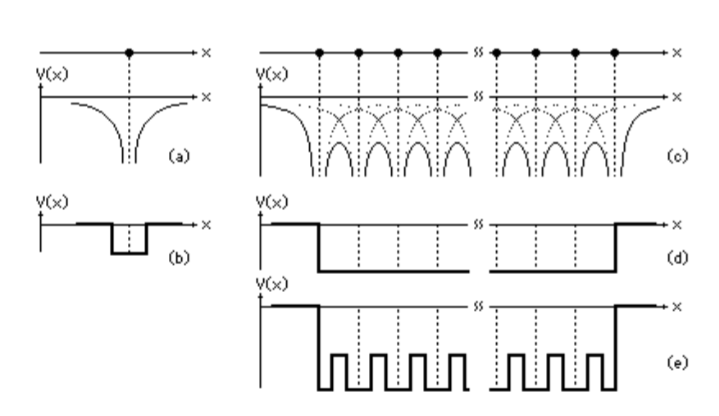
\includegraphics[width=0.5\textwidth]{puits.PNG}
    \caption{Graph du potentiel le long de l'axe $X$}
    \label{fig:puits}
\end{figure}

L'équation de Schrödinger pour l'étude d'un seul électron se réduit alors
\begin{equation}
    \left[-\frac{\hbar^2\nabla_i^2}{2m}+V(\Bar{r_i})+\sum_{j=1}^{Q}V_{ij}(\Bar{r_i})\right]\Phi(\Bar{r_i})=E_i\Phi(\Bar{r_i})
\end{equation}

Le potentiel dans lequel se balade l'électron est définit par la loi de Coulomb sur tous les noyaux
\begin{equation}
    V_{ij} = \frac{q^2}{4\pi\epsilon}\int\frac{|\Phi_j(\Bar{r_i})|^2}{|\Bar{r_i}-\Bar{r_j}|}d\Bar{r_j}
\end{equation}
Pour éviter de devoir calculer le potentiel pour chaque noyau on préférera se baser sur la périodicité du cristal.
\subsubsection{Modèles pour les électrons quasi-libres}
Utiliser le modèle de puits infinis est trop fastidieu, on souhaite faire une approximation pour obtenir un modèle plus facile d'utilisation.\\
\textbf{Modèle de Sommerfeld :} On assimile le modèle à un puits de potentiel constant le long du cristal (fig \ref{fig:puits}), ce modèle est trop simplificateur car il élimine totalement l'interaction avec les noyaux tant que l'électron ne rencontre pas les bords.\\
\textbf{Modèle de Krönig-Penney :} Modèle en carrés successifs, permet de ne pas perdre le propriétés du cristal dans le modèle (\href{fig:puits}{Figure \ref{fig:puits}}).\\
L'extension du second modèle à trois dimensions sera le modèle utilisé par le cours.
\subsubsection{ Modèle de Krönig-Penney d’un cristal unidimensionnel infini}
Soit le potentiel en carré
\begin{equation}
    \label{eq:KPequ}
    V(x) = \begin{cases}
    -V_0 &\text{ pour }  0\leq x\leq a\\
    V_1  &\text{ pour }  -b\leq x\leq 0
    \end{cases}
\end{equation}
\begin{figure}[H]
    \centering
    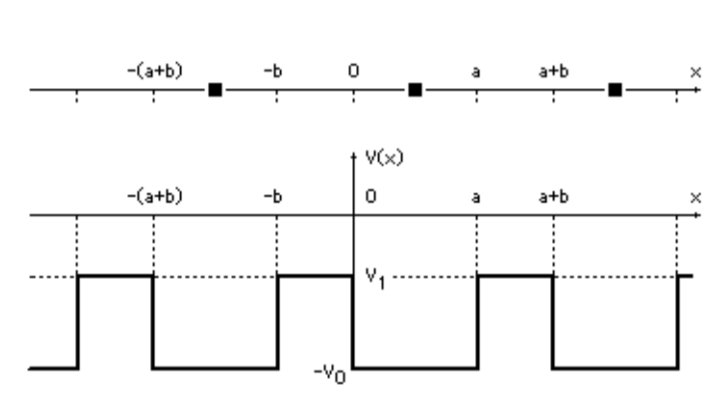
\includegraphics[width=0.5\textwidth]{ModeleKP.PNG}
    \caption{Modele de Krönnig-Penney \href{eq:KPequ}{Equation \ref{eq:KPequ}}}
    \label{fig:KPequ}
\end{figure}
Lorsqu'on lui applique le'équation de schrödinger on se retrouve avec deux équations différentielles
\begin{align}
    &\frac{-\hbar^2}{2m}\frac{d^2\phi(x)}{dx^2}-V_0\Phi(x) = E\Phi(x) &\text{ pour }  0\leq x\leq a\\
    &\frac{-\hbar^2}{2m}\frac{d^2\phi(x)}{dx^2}+V_1\Phi(x) = E\Phi(x) &\text{ pour }  -b\leq x\leq 0
\end{align}
On résout et obtient le système ci-dessous avec les paramètres 
\begin{gather}
    \alpha = \frac { 1 } { \hbar } \sqrt { 2 m \left( E + V _ { 0 } \right) } , \quad \alpha \geq 0\\
    \beta = \frac { 1 } { \hbar } \sqrt { 2 m \left( V _ { 1 } - E \right) } \quad , \quad \beta \geq 0\\
\end{gather}
\begin{align}
    &\frac { d ^ { 2 } \Phi } { d x ^ { 2 } } + \alpha ^ { 2 } \Phi = 0 , \quad &\Phi ( x ) = A e ^ { i \alpha x } + B e ^ { - i \alpha x } \quad \text { pour } \quad 0 \leq x \leq a\\
    &\frac { d ^ { 2 } \Phi } { d x ^ { 2 } } - \beta ^ { 2 } \Phi = 0 \quad , \quad &\Phi ( x ) = C e ^ { \beta x } + D e ^ { - \beta x } \quad \text { pour } - b < x < 0
\end{align}
Puisque la solution de l'équation de Schrödinger est périodique, la solution est une fonction de Bloch
\begin{equation}
    \Phi ( x ) = \left\{ \begin{array} { l l } { e ^ { i k x } u _ { a , k } ( x ) } & { , \quad 0 \leq x \leq a } \\ { e ^ { i k x } u _ { b , k } ( x ) } & { , - b < x < 0 } \end{array} \right.
\end{equation}
Le nombre d'onde $k$ doit être réel car sinon l'exponentielle ne serait pas bornée en $\pm \infty$.\\
En combinant les fonctions de Bloch et les solutions de l'équation de Schrödinger, pour ensuite isoler les fonctions de Bloch, on trouve 
\begin{gather}
    u _ { a , k } ( x ) = A e ^ { i ( \alpha - k ) x } + B e ^ { - i ( \alpha + k ) x } \quad \text { pour } \quad 0 \leq x \leq a\\
    u _ { b , k } ( x ) = C e ^ { ( \beta - i k ) x } + D e ^ { - ( \beta + i k ) x } \quad \text { pour } - b < x < 0
\end{gather}
Ces  fonctions doivent être continues et périodiques en leurs jonctions ce qui  nous donnes les quatre conditions suivantes
\begin{gather}
    u _ { a , k } ( 0 ) = u _ { b , k } ( 0 ), \quad
    \left( \frac { d u _ { a , k } } { d x } \right) _ { x = 0 } = \left( \frac { d u _ { b , k } } { d x } \right) _ { x = 0 }\\
    u _ { a , k } ( a ) = u _ { b , k } ( - b ), \quad
    \left( \frac { d u _ { a , k } } { d x } \right) _ { x = a } = \left( \frac { d u _ { b , k } } { d x } \right) _ { x = - b }
\end{gather}
On trouve les valeurs des coefficients $A$,$B$,$C$ et $D$ grâce au système ainsi obtenu
\begin{gather}
    A + B = C + D\\
    i ( \alpha - k ) A - i ( \alpha + k ) B = ( \beta - i k ) C - ( \beta + i k ) D\\
    e ^ { i ( \alpha - k ) a } A + e ^ { - i ( \alpha + k ) a } B = e ^ { - ( \beta - i k ) b } C + e ^ { ( \beta + i k ) b } D\\
    \begin{aligned} i ( \alpha - k ) e ^ { i ( \alpha - k ) a } A - i ( \alpha + k ) e ^ { - i ( \alpha + k ) a } B & =  ( \beta - i k ) e ^ { - ( \beta - i k ) b } C - ( \beta + i k ) e ^ { ( \beta + i k ) b _ { D } } \end{aligned}
\end{gather}
Pour résoudre ce système, il suffit de le mettre sous forme matriciel et d'imposer le déterminant nulle. On trouve ainsi la relation de dispersion
\begin{equation}
    \cos [ k ( a + b ) ] = \cos ( \alpha a ) \cosh ( \beta b ) + \frac { b \left( \beta ^ { 2 } - \alpha ^ { 2 } \right) } { 2 \alpha } \sin ( \alpha a ) \frac { \sinh ( \beta b ) } { \beta b }
\end{equation}
Nous devons maintenant modéliser la largeur des barrières de potentiel et la profondeur des puits. La modèle original a des barrières fines et des puits infinis, nous faisons donc tendre nos valeurs vers celles-ci
\begin{gather}
    \beta b =b \frac { \sqrt { 2 m \left( V _ { 1 } - E \right) } } { \hbar }  \rightarrow 0 \\
    \beta ^ { 2 } b = b \frac { 2 m \left( V _ { 1 } - E \right)  } { \hbar^2 } \rightarrow \frac { 2 m V _ { 1 } b } { \hbar ^ { 2 } }
\end{gather}
La valeur de E est bornée et donc $bE\rightarrow0$.\\
La relation de dispersion se réduit donc à 
\begin{equation}
    \cos ( k a ) = \cos ( \alpha a ) + P \frac { \sin ( \alpha a ) } { \alpha a } \quad \text{si} \quad P = \frac { m V _ { 1 } a b } { \hbar ^ { 2 } }
\end{equation}
On peut regrouper les équations sous cette forme pour mettre en évidence les bandes interdites
\begin{gather}
    f(\alpha a) = \cos ( \alpha a ) + P \frac { \sin ( \alpha a ) } { \alpha a }\\
    \cos(ka) = f(\alpha a)
\end{gather}
Puisque la valeur du cosinus ne peut pas sortir de l'intervalle $[-1;1]$, il existe des valeur pour lequel il n'y a pas de solution. On appelle ces valeurs bandes interdites. En représentant les valeur autorisées sur le graph de l'énergie on obtient les bandes d'énergie \href{fig:Ebands}{Figure \ref{fig:Ebands}}.
\begin{figure}[H]
    \centering
    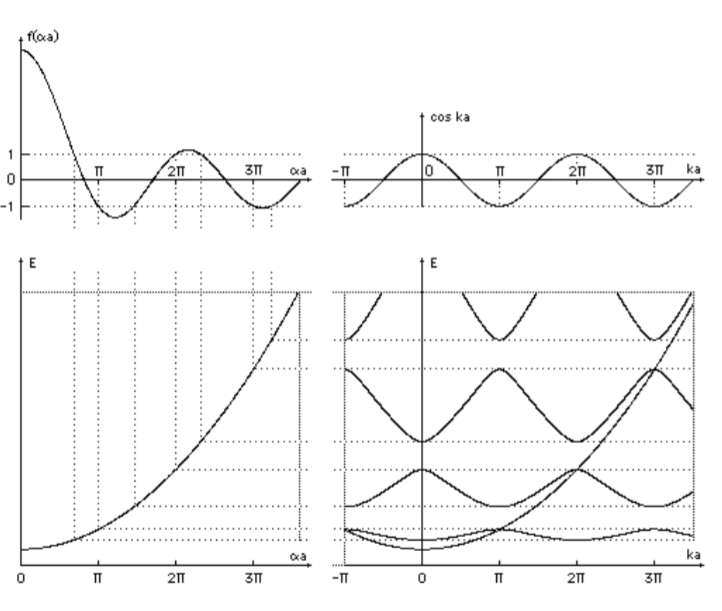
\includegraphics[width=0.6\textwidth]{Ebands.PNG}
    \caption{Solution Graphique de l'équation de dispersion}
    \label{fig:Ebands}
\end{figure}
On peut aussi en extraire la valeur de l'énergie en fonction du nombre d'onde à partir de la relation entre $\alpha$ et $E$.
\begin{gather}
    \alpha = \frac { 1 } { h } \sqrt { 2 m \left( E + V _ { 0 } \right) } \Longleftrightarrow E = - V _ { 0 } + \frac { ( \alpha h ) ^ { 2 } } { 2 m } = - V _ { 0 } + \frac { ( \alpha a ) ^ { 2 } \hbar ^ { 2 } } { 2 m a ^ { 2 } }
\end{gather}
\subsubsection{Valeurs limites de P}
\textbf{Lorsque $P\rightarrow0$ :} 
Les valeurs de $P$ très faibles correspondent à des barrières de potentiel très fines qui ne s'opposent que très peu aux électrons
\begin{equation}
    \cos ( k a ) = \cos ( \alpha a ) \quad , \quad \alpha \geq 0
\end{equation}
Ce modèle est équivalent au modèle de Sommerfeld et toutes les énergies au dessus du potentiel de référence sont nulles car on trouve $\alpha = | k |$
\begin{equation}
    E = - V _ { 0 } + \frac { \hbar ^ { 2 } k ^ { 2 } } { 2 m }
\end{equation}
\\
\textbf{Lorsque $P\rightarrow\infty$ :} 
La relation de dispersion se réduit à 
\begin{equation}
    \frac { \sin ( \alpha a ) } { \alpha a } = 0 \quad , \quad \alpha \geq 0
\end{equation}
Dont la solution est $\alpha a = n \pi ( n = 1,2,3 , \dots )$, et donc l'énergie a des états discrets de valeur
\begin{equation}
    E _ { n } = - V _ { 0 } + \frac { n ^ { 2 } h ^ { 2 } } { 8 m a ^ { 2 } } \quad , \quad n = 1,2,3 , \dots
\end{equation}
\begin{figure}[H]
    \centering
    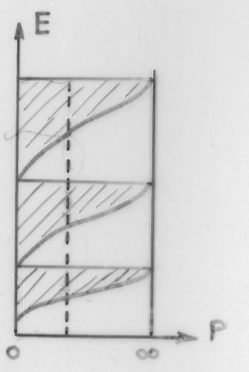
\includegraphics{Pvalues.PNG}
    \caption{Bandes d'énergies permises en fonction de P}
    \label{fig:Pgraph}
\end{figure}
Dans les deux cas on remarque que l'énergie est symétrique, ce qui est la source de l'existence de deux particules dans un même état d'énergie (principe d'exclusion de Pauli).
%\subsubsection{Extension au domaine temporel}
%L'équation du comportement de l'électron dans un cristal dépendante du temps s'écrit en toutes généralité 
\subsubsection{Bandes d'énergies d'un cristal fini}
Un cristal n'est pas infini et doit donc être modélisé par une longueur $L = aN$, avec $a$ la distance entre deux mailles et $N$ le nombre. Nous partons de l'équation d'onde temporelle
\begin{equation}
    \Psi ( x , t ) = u _ { k } ( x ) e ^ { i \left[ k x - E _ { n } ( k ) t / h \right] } \quad , \quad ( - \pi / a < k \leq + \pi / a )
\end{equation}
Nous lui appliquons la condition cyclique de Born-von Karman, à savoir que la translation correspond à l'opération identité.
\begin{gather}
    \Psi ( x + L , t ) = \Psi ( x , t ) =\\
    u _ { k } ( x ) e ^ { i \left[ k x - E _ { n } ( k ) t / h \right] } = u _ { k } ( x+L ) e ^ { i \left[ k (x+L) - E _ { n } ( k ) t / h \right] }\\
    = u _ { k } ( x ) e ^ { i \left[ k x - E _ { n } ( k ) t / h \right] }e^{ikL}
\end{gather}
Il s'avère que si l'identité doit être respecté, le terme ainsi obtenu doit valoir $1$.
\begin{equation}
    e^{ikL} = =e^{ikNa} =1 \Leftrightarrow 2n\pi =kNa
\end{equation}
On se retrouve avec une liste de valeurs possible pour $k$
\begin{equation}
    k = \frac { 2 \pi n } { a N } \quad , \quad n = 0 , \pm 1 , \pm 2 , \pm 3 , \ldots , \pm \frac { N - 1 } { 2 } , \pm \frac { N } { 2 }
\end{equation}
On peut de cette équation déduire la densité d'états qui permettra de calculer le nombre d'états possible pour un électrons en fonction de la taille du dispositif.
\begin{equation}
    n ( k ) = \frac { a N } { 2 \pi } = \frac { L } { 2 \pi }
\end{equation}
Par extension au volume on trouve
\begin{equation}
    n ( \overline { k } ) = \frac { \mathcal{V} } { 8 \pi ^ { 3 } }
\end{equation}
avec $\Bar{k}$ une direction $(k_x,k_y,k_z)$ dans le cristal.\\
L'étude des bandes d'énergies à trois dimensions permet également de mettre en évidence des situations de recouvrement de bandes d'énergie. On dira d'un état qu'il est dégénéré lorsque pour des valeurs $k$ différents il existe de valeur $E(k)$ égales.\\

\subsection{Modèle de l'électron et du trou}
\subsubsection{Vitesse de l'électron dans le cristal}
On munit la fonction d'onde d'un terme d'amplitude associé à chaque direction. En intégrant cette expression dans toutes les directions on obtient finalement 
\begin{equation}
    \Psi ( \overline { r } , t ) = u _ { \overline { k } _ { o } } ( \overline { r } ) \int _ { Z B } A ( \overline { k } ) e ^ { i \left[ \overline { k } \cdot \overline { r } - E _ { n } ( \overline { k } ) t / \hbar \right] } d \overline { k }
\end{equation}
Ce qui correspond à la fonction d'onde d'un groupe d'électrons.\\
Pour trouver la vitesse de groupe, on dérive la fonction de l'énergie dans toutes les directions
\begin{equation}
    \overline { v } _ { g } ( \overline { k } ) = \frac { 1 } { \hbar } \nabla  _ { \overline { k } } E _ { n } ( \overline { k } )
\end{equation}
Dans le cas du modèle de Sommerfeld on obtient une simple expression de la vitesse d'unn électron dans un puit de potentiel $v _ { g } = \hbar k / m$. On peut appliquer le résultat du modèle de Sommerfeld aux valeurs éloignées de $k = \pm \pi/a$, ensuite en examinant les limites $k = \pm \pi/a$ au travers de la dérivé de la relation de dispersion

\begin{equation}
    - a \sin ka \cdot d k =\frac { d } { d \alpha } \left( \cos \alpha a + P \frac { \sin \alpha a} { \alpha a } \right) \cdot \frac { d \alpha } { d E } \cdot \frac { d E } { d k } \cdot d k
\end{equation}

On injecte $k = \pm \pi/a$

\begin{equation}
    - a \sin  \frac{\pi}{a}a \cdot d k = 0 = \frac { d } { d \alpha } \left( \cos \alpha a + P \frac { \sin \alpha a} { \alpha a } \right) \cdot \frac { d \alpha } { d E } \cdot \frac { d E } { d k } \cdot d k
\end{equation}
On remarque que tous les termes sont non-nulle sauf $\frac{dE}{dk}$ qui est donc forcément nulle pour maintenir l'égalité.\\
En se basant sur l'analyse précédente, on peut analyser graphiquement la forme de la vitesse \href{fig:vgspeed}{Figure \ref{fig:vgspeed}}.\\
\begin{figure}[H]
    \centering
    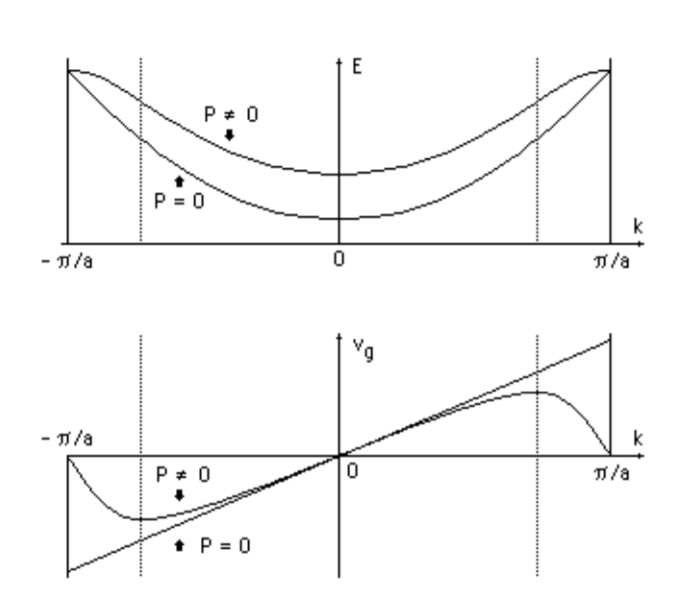
\includegraphics[width=0.5\textwidth]{speed.PNG}
    \caption{Vitesse de groupe des électrons au regard de la fonction de l'énergie}
    \label{fig:vgspeed}
\end{figure}
L'analyse de la vitesse permet aussi de dégager certains phénomènes, le premier étant la réflexion de Bragg à la limite de la zone de Brillouin. Celà est du au fait qu'un électron ayant un nombre d'onde supérieur à $\pi/a$ ne peut se propager dans un milieu de période $a$. La fonction d'onde est donc stationnaire et de vitesse nulle en se point.

\subsubsection{Masse effective de l'électron}
On se base sur le théorème de masse effective pour continuer la démonstration. Celui-ci stipule que si les forces extérieur au cristal sont négligeables face à celles du réseau, on pour utiliser le modèle de masse effective pour l'électron. L'électron est alors considéré comme une particule de masse variable différente de sa véritable masse dont le modèle inclut tout les phénomènes dûs au réseau cristallin. Nous la définissons sur base d'une force constante exercé sur le cristal. L'énergie d'un déplacement du à une force est donné par
\begin{gather}
    d E = \overline { F } \cdot \overline { v } _ { g } d t\\
    \frac { d E } { d t } = \operatorname { grad } _ { \overline { k } } E \cdot \frac { d \overline { k } } { d t } = \frac { 1 } { \hbar } \overline { F } \cdot \nabla  _ { \overline { k } } E
\end{gather}
On trouve par identification
\begin{equation}
    \hbar \frac { d \overline { k } } { d t } = \overline { F }
\end{equation}
On s'intéresse maintenant à l'accélération de l'électron en fonction de la masse effective $\mathbf { m } ^ { * } = \Bar{F}/a$
\begin{equation}
    \frac { d \overline { \nu } _ { g } } { d t } = \frac { 1 } { \hbar ^ { 2 } } \operatorname { grad } _ { \overline { k } } \left( \operatorname { grad } _ { \overline { k } } E \cdot \overline { F } \right) = \left( \frac { 1 } { \mathbf { m } ^ { * } } \right) \cdot \overline { F }
\end{equation}
Le gradient carré d'un vecteur est un tenseur, on trouve donc la masse effective en fonction de l'énergie
\begin{equation}
    \frac { 1 } { \mathbf { m } ^ { * } } = \frac { 1 } { \hbar ^ { 2 } } \left| \begin{array} { c c c } { \frac { \partial ^ { 2 } E } { \partial k _ { 1 } ^ { 2 } } } & { \frac { \partial ^ { 2 } E } { \partial k _ { 1 } \partial k _ { 2 } } } & { \frac { \partial ^ { 2 } E } { \partial k _ { 1 } \partial k _ { 3 } } } \\ { \frac { \partial ^ { 2 } E } { \partial k _ { 2 } \partial k _ { 1 } } } & { \frac { \partial ^ { 2 } E } { \partial k _ { 2 } ^ { 2 } } } & { \frac { \partial ^ { 2 } E } { \partial k _ { 2 } \partial k _ { 3 } } } \\ { \frac { \partial ^ { 2 } E } { \partial k _ { 3 } \partial k _ { 1 } } } & { \frac { \partial ^ { 2 } E } { \partial k _ { 3 } \partial k _ { 2 } } } & { \frac { \partial ^ { 2 } E } { \partial k _ { 3 } ^ { 2 } } } \end{array} \right|
\end{equation}
La \href{fig:meffe}{Figure \ref{fig:meffe}} illustre le comportement de la masse effective unidimensionnelle. 
\begin{figure}[H]
    \centering
    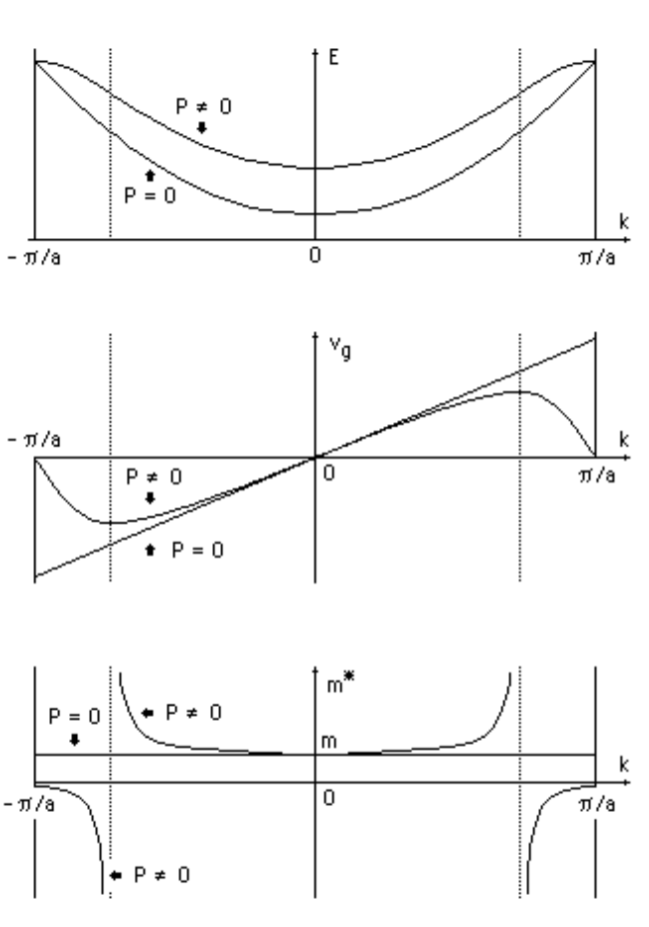
\includegraphics[width=0.5\textwidth]{meffe.PNG}
    \caption{Variation de la masse effective en fonction de la vitesse et de l'énergie}
    \label{fig:meffe}
\end{figure}
On remarque que la masse effective est égale à la masse de l'électron dans la zone où le modèle de Sommerfeld est applicable puisque celui-ci correspond à la particule libre. On peut interpréter le comportement de l'électron dans le cristal comme un électron libre de masse effective $m^*$.\\
On peut réécrire l'énergie en fonction de la masse effective grâce à un développement en série autour de $\Bar{k_0}$ du deuxième ordre
\begin{equation}
    \frac { 1 } { m _ { i } ^ { * } } = \frac { 1 } { \hbar ^ { 2 } } \left( \frac { \partial ^ { 2 } E } { \partial k _ { i } ^ { 2 } } \right) _ { \overline { k } _ { o } }
\end{equation}
En partant de ce résultat on peut réécrire la formule de l'énergie
\begin{equation}
    E _ { n } ( \overline { k } ) = E _ { n } \left( \overline { k } _ { o } \right) + \frac { \hbar ^ { 2 } } { 2 } \sum _ { i = 1 } ^ { 3 } \frac { 1 } { m _ { i } ^ { * } } \left( k _ { i } - k _ { o , i } \right) ^ { 2 }
\end{equation}
Les masses effectives dépendent de la direction, on utilise la forme de la zone d'énergie constante pour définir le type de masse effective. Ce sont des ellipsoïdes de révolution centrés en $\Bar{k_0}$.

\subsubsection{Trou positif}
Soit la densité de courant d'une charge $-q$ dans un volume $V$
\begin{equation}
    \overline { J } = - q \overline { v } _ { g } / V
\end{equation}
En utilisant la fonction de distribution des électrons $f(\Bar{k})$ et la densité d'états permis $V/8\pi^3$ on peut calculer le nombre d'électrons occupant les états permis
\begin{equation}
    n(d\Bar{k}) = 2 . f ( \overline { k } ) \cdot \left(\frac{V}{ 8 \pi ^ { 3 } }\right) \cdot d \overline { k }
\end{equation}
En utilisant cette expression on peut calculer la densité de courant du au mouvement de l'ensemble des électrons dela bande permise.  
\begin{equation}
    \overline { J } = - \frac { q } { 4 \pi ^ { 3 } } \int _ { Z B } f ( \overline { k } ) \overline { v } _ { g } ( \overline { k } ) d \overline { k }
\end{equation}
Sachant que $\overline { v } _ { g } ( \overline { k } ) $ est forcément symétrique, on remarque qu'une bande complètement remplie ne contribue pas à un courant car celui-ci est nulle.\\
Analysons maintenant le cas d'une bande rempli à un électron près, l'équation deviens
\begin{equation}
    \overline { J } = 0 - \left[ - q \overline { v } _ { g } ( \overline { k } ) / V \right] = + q \overline { v } _ { g } ( \overline { k } ) / V
\end{equation}
Ce qui est l'équivalent d'une bande vide contenant un "anti-électron" ce qu'on appellera un trou positif. Le trou est de charge opposé mais de même vitesse qu'un électron. On peut mettre en équation la densité de trous positif la bande de conduction
\begin{equation}
n ( d \overline { k } ) = 2 . \left[1-f ( \overline { k } )\right] \cdot \left( \frac { V } { 8 \pi ^ { 3 } } \right) \cdot d \overline { k }
\end{equation}
et en utilisant cette équation pour calculer al densité de courant on se retrouve avec
\begin{equation}
    \overline { J } = + \frac { q } { 4 \pi ^ { 3 } } \int _ { Z B } [ 1 - f ( \overline { k } ) ] \overline { v } _ { g } ( \overline { k } ) d \overline { k }
\end{equation}
En réutilisant les équation de masse effective dans le cas du trou positif on trouve
\begin{equation}
    \frac { d \overline { \nu } _ { g } } { d t } = \frac { 1 } { \mathbf { m } ^ { * } } \cdot \overline { F } = \frac { 1 } { \mathbf { m } ^ { * } } \cdot ( - q \overline { \mathcal { E } } )= \left( - \frac { 1 } { m ^ { * } } \right) \cdot ( + q \overline { \mathcal { E } } )
\end{equation}
Le trou positif est donc de masse effective opposée à l'électron, charge opposée à l'électron, la courbe de sa vitesse en fonction de l'énergie est également inverse.

\subsection{Bandes d'énergies}
\subsubsection{ Distinction entre isolants, semiconducteurs et
métaux}
La distinction entres les différents types de conducteurs dépend de leurs bandes d'énergies. On distingue un conducteur (un métal) d'un isolant par le fait qu'il y a une bande d'énergie que partiellement rempli d'électrons qui pouront contribuer au courant.
\begin{figure}[H]
    \centering
    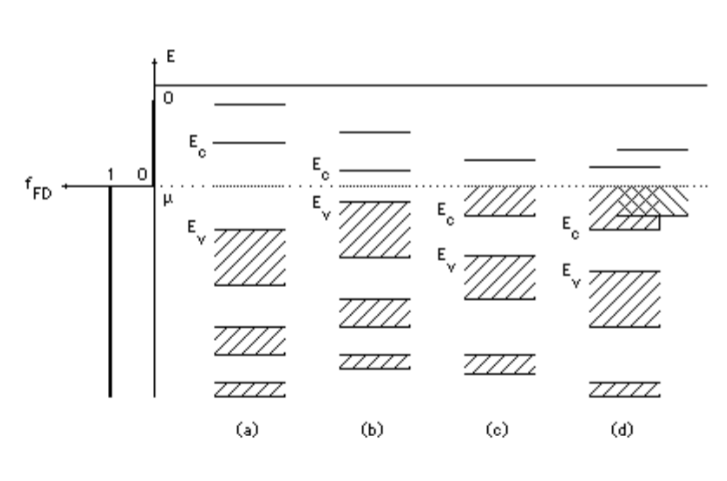
\includegraphics[width=0.5\textwidth]{bandEx.PNG}
    \caption{Bandes d’énergie à 0 K d’un isolant (a), d’un semiconducteur
(b) et d’un métal (c), (d). La statistique de Fermi-Dirac à gauche indique le pourcentage$/100$ d'occupation de la bande}
    \label{fig:bandEx}
\end{figure}
Sur la \href{fig:bandEx}{Figure \ref{fig:bandEx}}, les matériaux sont à 0K et n'ont donc aucun éparpillement des électrons autour de la statistique de Fermi-Dirac, car ceux-ci occupent toujours les bandes d'énergies les plus basses en premier à cette température.\\
Le semiconducteur se caractérise par la présence d'un band gap $E_g = E_v - E_c$ entre la bande de conduction et la bande de valence faible, atour de $1eV$. Dans le cas d'un isolant, le band gap sera $E_g > 5eV $ de manière à ce que aucun électron ne pourra  atteindre la bande de conduction par agitation thermique, ce qui est possible pour un semiconducteur. 

\subsubsection{Densité d'états permis}
On peut calculer la densité d'électrons dans une bande d'énergie à partir de la distribution $f(\Bar{k})$ et la densité d'états permis $n(\Bar{k}) = 1/8\pi^3$ grâce à 
\begin{equation}
n = 2 \int _ { Z B } n ( \overline { k } ) f ( \overline { k } ) d \overline { k }
\end{equation}
Idem pour les trous avec $1 - f ( \overline { k } )$.\\
La fonction de distribution $f$ est donnée par le potentiel chimique $\mu$ et l'énergie de la bande,  ici la fonction de Fermi-Dirac
\begin{equation}
    f ( \overline { k } ) = \frac { 1 } { 1 + e^\frac{E _ { n } ( \overline { k } ) - \mu}{kT} }
\end{equation}
On préfèrera utiliser l'énergie directement, plutôt que le nombre d'onde.\\
On connaît le lien entre l'énergie de la bande à ses extrema $k_{m,i}$ grâce à la relation 
\begin{equation}
    E ( \overline { k } ) = E _ { c } \left( \overline { k } _ { m } \right) + \frac { \hbar ^ { 2 } } { 2 } \sum _ { i = 1 } ^ { 3 } \frac { 1 } { m _ { i } ^ { * } } \left( k _ { i } - k _ { m , i } \right) ^ { 2 }
\end{equation}
Cette relation permet de changer les bornes d'intégration pour utiliser l'énergie plutôt que la surface de Brioullin.\\
Ensuite on calculera la taille approximative grâce aux longueurs des ellipsoïdes pour se débarrasser de $\Bar{k}$ 
\begin{equation}
    L _ { i } = \frac{\sqrt{2 m _ { i } ^ { * } \left( E - E _ { c } \right)}}{\hbar}
\end{equation}
Ensuite on utilise la formule du volume de l'ellipsoïde et l'équation de la densité d'état (40) pour trouver le nombre total d'états permis
\begin{equation}
    M ( E ) = \frac { 1 } { 8 \pi ^ { 3 } } \frac { 4 \pi } { 3 } L _ { 1 } L _ { 2 } L _ { 3 } = \frac { 1 } { 6 \pi ^ { 2 } \hbar ^ { 3 } } \left[ 2 \left( E - E _ { c } \right) \right] ^ { 3 / 2 } \sqrt{m _ { 1 } ^ { * } m _ { 2 } ^ { * } m _ { 3 } ^ { *}}
\end{equation}
On préférera utiliser la masse effective de densité d’états de la bande de conduction pour simplifier la notation, en utilisant $\kappa_c$ le nombre de minimas équivalents 
\begin{equation}
m _ { c } = \kappa _ { c } ^ { 2 / 3 } \sqrt[3]{m _ { 1 } ^ { * } m _ { 2 } ^ { * } m _ { 3 } ^ { *}}
\end{equation}
On cherche à calculer $N(E)dE$
\begin{equation}
N ( E ) d E = \frac{dM(E)}{dE}dE = \frac { 3\sqrt { m _ { 1 } ^ { * } m _ { 2 } ^ { * } m _ { 3 } ^ { * } } } { 6 \pi ^ { 2 } \hbar ^ { 3 } } \sqrt{2}\left( E - E _ { c } \right) ^ { 1 / 2 } dE
\end{equation}
On trouve ainsi finalement l'expression
\begin{equation}
    N _ { c } ( E ) = \frac { \sqrt { m _ { c } ^ { 3 } \left( E - E _ { c } \right) } } { \sqrt { 2 } \pi ^ { 2 } \hbar ^ { 3 } }
\end{equation}
la densité d'états permis.\\
Pour trouver le nombre d'électrons, il suffit d'intégrer sur l'énergie
\begin{equation}
n = 2 \int _ { E _ { c } } ^ { E _ { M c } } N _ { c } ( E ) f ( E ) d E
\end{equation}
\begin{figure}[H]
    \centering
    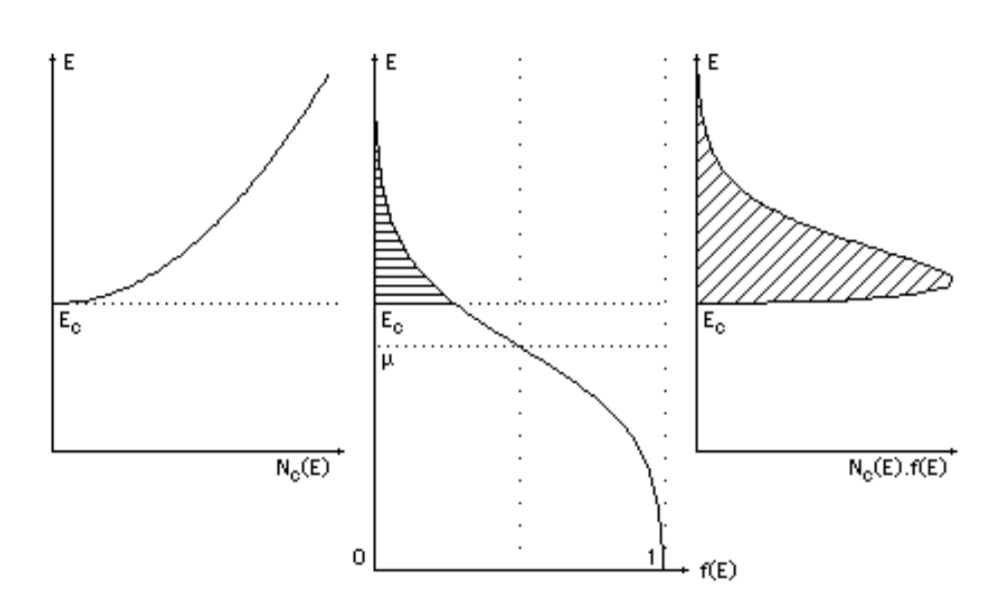
\includegraphics[width=0.8\textwidth]{distrFD.PNG}
    \caption{Valeur de l'énergie, distribution de Fermi-Dirac, Densité d'états permis}
    \label{fig:distB}
\end{figure}
Le calcule de la densité de trous se fait par le même raisonnement que pour les électrons :
\begin{gather}
    E ( \overline { k } ) = E _ { v } \left( \overline { k } _ { M } \right) - \frac { \hbar ^ { 2 } } { 2 } \sum _ { i = 1 } ^ { 3 } \frac { 1 } { m _ { i } ^ { * } } \left( k _ { i } - k _ { M , i } \right) ^ { 2 }\\
    { N _ { v } ( E ) = \frac { \sqrt { m _ { v } ^ { 3 } \left( E _ { v } - E \right) } } { \sqrt { 2 } \pi ^ { 2 } \hbar ^ { 3 } } } \\ { m _ { \nu } = \kappa _ { v } ^ { 2 / 3 } \left( m _ { 1 } ^ { \prime * } m _ { 2 } ^ { \prime * } m _ { 3 } ^ { \prime * } \right) ^ { 1 / 3 } } \\p = 2 \int _ { E _ { m v } } ^ { E _ { v } } N _ { v } ( E ) [ 1 - f ( E ) ] d E
\end{gather}
\begin{figure}[H]
    \centering
    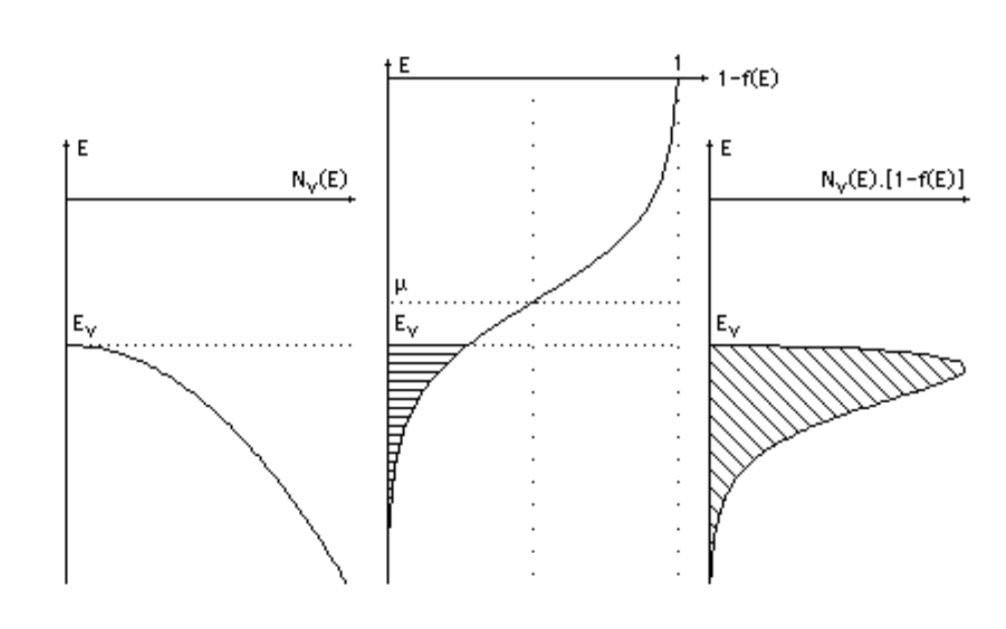
\includegraphics[width=0.8\textwidth]{distrFDT.PNG}
    \caption{Distribution pour les trous}
    \label{fig:DistrT}
\end{figure}
%%%%%%%%%%%%%%%%%%%%%%%%%%%%%%%%%%%%%%%%%%%%%%%%%%%%%%%%%%%%%%%%%
\subsection{Densités de porteurs}
Du chapitre précédent, nous savons que la densité d'électrons et de trous en fonction de l'énergie sont respectivement données par 
\begin{equation}
  { n } = \frac { \sqrt { 2   { m } _ {   { c } } ^ { 3 } } } { \pi ^ { 2 } \hbar ^ { 3 } } \int _ { 0 } ^ { \infty } \frac { \sqrt {   { E } -   { E } _ {   { c } } } } { 1 +   { e } ^ { (   { E } - \mu ) /   { kT } }  }  { d } \left(   { E } -   { E } _ {   { c } } \right)
\end{equation}
\subsubsection{Cas d'un métal}
Dans le cas d'un métal, la bende de conduction est en partie remplie. Le développement en série de l'énergie autour du minima $\Bar{k_m}$ n'est valable que proche de ce minima, l'approximation est donc fausse dans le cas d'un métal.\\
On remarque que la distribution de Fermi-Dirac devient rapidement négligeable lorsque les valeurs de $E$ dépassent le potentiel chimique $\mu$ \href{fig:FDdistr}{Figure \ref{fig:FDdistr}}.

\begin{figure}[H]
    \centering
    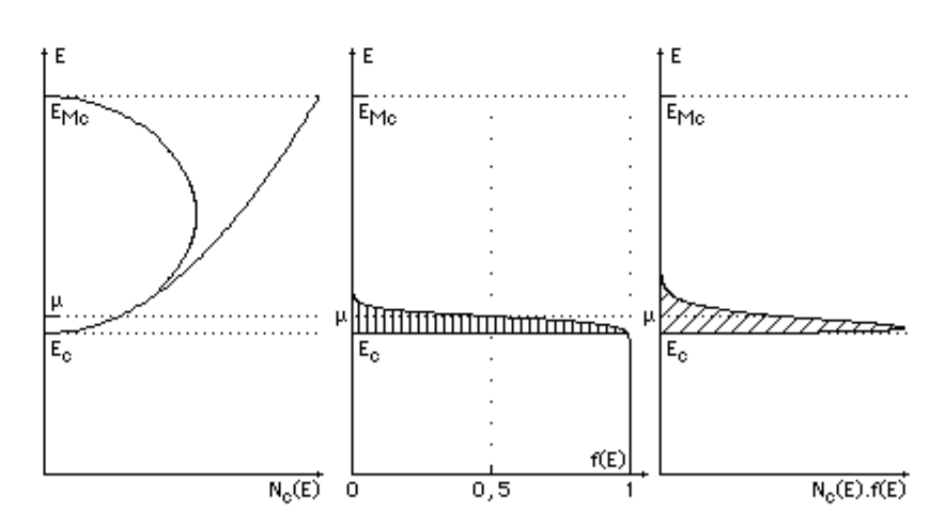
\includegraphics[width=0.8\textwidth]{Mdistr.PNG}
    \caption{Distribution des électrons dans un métal}
    \label{fig:FDdistr}
\end{figure}

On développe l'intégrale  en série pour plus facilement l'intégrer
\begin{gather}
n = \frac { \sqrt { 2 m _ { c } ^ { 3 } } } { \pi ^ { 2 } \hbar ^ { 3 } } \left[ \int _ { 0 } ^ { \mu - E _ { c } } \sqrt { E - E _ { c } } d \left( E - E _ { c } \right) + \frac { 1 } { 2 } \frac { 1 } { \sqrt { \mu - E _ { c } } } \frac { ( \pi k T ) ^ { 2 } } { 6 } + \ldots \right]\\
n = \frac { \sqrt { 2 m _ { c } ^ { 3 } } } { 3 \pi ^ { 2 } \hbar ^ { 3 } } \left[ 2 \sqrt { \left( \mu - E _ { c } \right) ^ { 3 } } + \frac { ( \pi k T ) ^ { 2 } } { 4 \sqrt { \mu - E _ { c } } } + \ldots \right]
\end{gather}
On trouve finalement une relation directe entre le nombre d'électrons et l'énergie $\mu - E_c$ valable à $0K$ en négligeant le second terme
\begin{gather}
n = \frac { \sqrt { 2 m _ { c } ^ { 3 } } } { 3 \pi ^ { 2 } \hbar ^ { 3 } } 2 \sqrt { \left( \mu - E _ { c } \right)_{T=0} ^ { 3 } }\\
\left( \mu - E _ { c } \right) _ {T= 0 } = \frac { \hbar ^ { 2 } } { 8 m _ { c } } \left( \frac { 3 n } { \pi } \right) ^ { 2 / 3 }
\end{gather}
On étend cette analyse au cas ou la température est différente de $0K$ en ajoutant le terme manquant. Le rapport des énergies dans le cas d'un seul électron permet de mettre en évidence le facteur
\begin{equation}
n = 1 + \frac { ( \pi k T ) ^ { 2 } } { 4 \sqrt { \mu - E _ { c } } } \quad,\quad \frac { \mu - E _ { C } } { \left( \mu - E _ { C } \right) _ { 0 } } = \frac{n_{T=0}^{2/3}}{n_{T\neq0}^{2/3}} = \frac { 1 } { \left[ 1 + \frac { \pi ^ { 2 } } { 8 } \left( \frac { k T } { \mu - E _ { c } } \right) ^ { 2 } \right] ^ { 2 / 3 } }
\end{equation}
En mettant en évidence le facteur on trouve
\begin{equation}
\mu - E _ { c } = \left( \mu - E _ { c } \right) _ { 0 } \left\{ 1 - \frac { \pi ^ { 2 } } { 12 } \left[ \frac { k T } { \left( \mu - E _ { c } \right) _ { 0 } } \right] ^ { 2 } \right\}
\end{equation}
Ce terme est très petit, l'énergie de fermi d'un métal ne varie que très peu avec la température.\\
On définit la température Fermi comme
\begin{equation}
T _ { F } =\frac{ \mu - E _ { c } }{k} \quad 
\end{equation}
\subsubsection{Effet Schottky}
On peut augmenter l'émission d'électrons à la surface d'un métal à l'aide d'un champ électrique, c'est ce qu'on appelle l'effet Schottky. Pour examiner cet effet, on analysera les effets électriques lors de l'extraction. La force de rappel d'un électron à une distance $x$ de son proton est
\begin{equation}
F = - \frac{q ^ { 2 }}{  4 \pi \epsilon _ { o } ( 2 x ) ^ { 2 }}
\end{equation}
Le champ électrique du à cette force est 
\begin{equation}
E _ { 1 } ( x ) = - \frac { q ^ { 2 } } { 16 \pi \epsilon _ { o } x }
\end{equation}
Cette interprétation ne vaut que pour les valeurs supérieur à la distance interatomique. On découvre qu'il existe un maximum $x_0$ pour lequel l'énergie potentielle de l'électron est maximale \href{Schottky.PNG}{Figure \ref{fig:Schottky}}
\begin{gather}
E _ { 3 } ( x ) = E _ { 1 } ( x ) + E _ { 2 } ( x ) \quad \text { avec }\quad E _ { 2 } ( x ) = - q \mathcal{E} x \qquad \text{le champ électrique}\\
E _ { 3 } \left( x _ { o } \right) = - q \sqrt { \frac { q \mathcal { E } } { 4 \pi \epsilon _ { o } } } \qquad \text{au point particulier} \qquad x _ { o } = \sqrt { \frac { q } { 16 \pi \epsilon _ { o } \mathcal { E } } }
\end{gather}
Ce maxima est la différence de travail d'extraction nécessaire à passer la barrière de potentiel. Celui-ci est donc diminué de cette valeur
\begin{equation}
W ^ { \prime } = W - \Delta W = - \mu - \Delta W = - \mu - q \sqrt { \frac { q \mathcal { E } } { 4 \pi \epsilon _ { o } } }
\end{equation}

\begin{figure}[H]
    \centering
    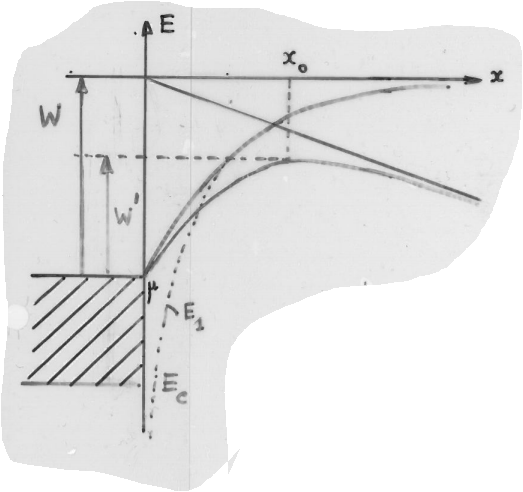
\includegraphics[width=0.6\textwidth]{Schottky.PNG}
    \caption{Potentiel et champ électrique à l'extraction}
    \label{fig:Schottky}
\end{figure}

\subsubsection{Émission thermoionique}

L'effet Schottky est mesuré à température nulle, en pratique ce n'est pas le cas. En repartant de l'expression de l'énergie et de la vitesse 
\begin{equation}
E = E _ { c } + \frac { \hbar ^ { 2 } } { 2 m ^ { * } } \sum _ { i = 1 } ^ { 3 } \left( k _ { i } - k _ { m , i } \right) ^ { 2 }\qquad,\qquad \overline { v } = \frac { 1 } { \hbar } \operatorname { grad } _ { \overline { k } } E ( \overline { k } ) = \frac { \hbar } { m ^ { * } } \left( \overline { k } - \overline { k } _ { m } \right)
\end{equation}
et en utilisant leur relation
\begin{equation}
E = E _ { c } + \frac { 1 } { 2 } m ^ { * } \overline { v } ^ { 2 } = E _ { c } + \frac { 1 } { 2 } m ^ { * } \left( v _ { x } ^ { 2 } + v _ { y } ^ { 2 } + v _ { z } ^ { 2 } \right)
\end{equation}
on peut construire l'expression du nombre d'électrons $P(E)$ ayant une énergie suffisante pour être extrait du métal (attention à la relation $m _ { c } = \kappa _ { c } ^ { 2 / 3 } m ^ { * }$)
\begin{equation}
P ( E ) d E = 2 N _ { c } ( E ) f ( E ) d E = \frac { \sqrt { 2 \left( E - E _ { c } \right) m _ { c } ^ { 3 } } d E } { \pi ^ { 2 } \hbar ^ { 3 } \left[ 1 + e ^ { ( E - \mu ) / k T } \right] }
\end{equation}
En faisant le changement de variable dans l'expression précédente
\begin{equation}
P \left( v _ { x } , v _ { y } , v _ { z } \right) d v _ { x } d v _ { y } d v _ { z } = \frac { P ( | \overline {  { v } } | ) d | \overline {  { v } } | } { 4  { \pi } | \overline { { v } } | ^ { 2 } d | \overline {  { v } } | }d v _ { x } d v _ { y } d v _ { z }=\frac { \kappa _ { c } m ^ { * 3 } d v _ { x } d v _ { y } d v _ { z } } { 4 \pi ^ { 3 } \hbar ^ { 3 } \left[ 1 + e ^ { \left( E _ { c } + W + \frac { 1 } { 2 } m ^ { * } \overline { v } ^ { 2 } \right) / k T } \right] }
\end{equation}
La vitesse correspondant au seuille énergétique est donné grâce à la relation trouvé pour l'effet Schottky
\begin{equation}
v _ { x o } = \sqrt { 2 \left( - E _ { c } - \Delta W \right) / m ^ { * } }
\end{equation}
Par définition, la densité de courant est donnée par
\begin{equation}
J = - q \int _ { v _ { x } o } ^ { \infty } \int _ { - \infty } ^ { \infty } \int _ { - \infty } ^ { \infty }v_xP \left( v _ { x } , v _ { y } , v _ { z } \right) d v _ { x } d v _ { y } d v _ { z }
\end{equation}
On peut utiliser l'approximation de Maxwell-Boltzmann puisque $E - \mu = E _ { c } + W + \frac { 1 } { 2 } m ^ { * } \overline { v } ^ { 2 } \gg k T$
\begin{equation}
J = - \frac { q \kappa _ { c } m ^ { * 3 } } { 4 \pi ^ { 3 } \hbar ^ { 3 } } e ^ { - \left( E _ { c } + W \right) / k T } \int _ { v _ { x o } } ^ { \infty } v _ { x } e ^ { - m ^ { * } v _ { x } ^ { 2 } / 2 k T } d v _ { x }\int _ { - \infty } ^ { \infty } \int _ { - \infty } ^ { \infty } e ^ { - m ^ { * } \left( v _ { y } ^ { 2 } + v _ { z } ^ { 2 } \right) / 2 k T } d v _ { y } d v _ { z }
\end{equation}
On obtient la loi de Richardson-Dusham
\begin{gather} 
{ J = - A _ { o } T ^ { 2 } e ^ { - W ^ { \prime } / k T } = - A _ { o } T ^ { 2 } e ^ { - W / k T } e ^ { \frac { q } { k T } \sqrt { \frac { q Z } { 4 \pi c _ { o } } } } } \\
{ A _ { o } = 4 \pi m ^ { * } q \kappa _ { c } k ^ { 2 } / h ^ { 3 } } 
\end{gather}
La densité décroit exponnentiellement en fonction de $W/kT$ et croit exponentiellement en fonction du champ électrique.\\
Le modèle ne prend pas en compte l'effet tunnel et n'est donc pas valable pour des champ électriques grand, car la barrière de potentiel est alors très fine et la probabilité de la traverser est alors non-négligeable. Il faut alors corriger le modèle en lui sommant la densité dû à l'effet tunnel.
\subsubsection{Potentiel de contact}
Au contact entre deux métaux, puisque leur potentiel thermodynamique et leur bandes de conductions sont différents. La différence de bandes d'énergie fait migrer les électrons d'un métal à l'autre car ceux-ci migrent vers l'état énergétique le plus bas. La différence en densité d'électrons crée quant à lui un champ électrique créant un potentiel de rappel. Un équilibre se créé 
\begin{gather}
    \overline { F } _ { 1 } = - \nabla  _ { \overline { r } } \mu _ { c } ( \overline { r } )\qquad    \overline { F } _2 = - q \mathcal { E } = + q \nabla  _ { \overline { r } } \Psi ( \overline { r } )\\
    \Psi _ { o } = \Psi \left( \overline { r } _ { 1 } \right) - \Psi \left( \overline { r } _ { 2 } \right)\\
    \overline { F } _1 + \overline { F } _2 = 0 \quad\Leftrightarrow\quad \operatorname { grad } _ { \overline { r } } \left( \mu _ { c } - q \Psi \right) = 0\\
    \mu _ { c } ( \overline { r } ) - q \Psi ( \overline { r } ) = \mu = \text{constant}
\end{gather}
On définit ainsi $\mu$ comme la constante énergétique séparant les deux métaux et $\Psi_0$ la différence de potentiel de contact. Ce dernier est définit comme
\begin{equation}
q \Psi _ { o } = W _ { 2 } - W _ { 1 } = \mu _ { 1 } - \mu _ { 2 }
\end{equation}

\section{Semiconducteur}
\subsection{Bandes d’énergie d’un
semiconducteur}
\subsubsection{Niveaux extrinsèques d’énergie dans la bande
interdite}
Il existe plusieurs types d'impuretés et phénomènes dans le cristal qui ont chacune leurs effets.\\
\textbf{Cristal Fini :} La fin du cristal correspond à une interruption de la périodicité. Par les conditions cycliques de Born-von Karman on élimine
cette difficulté au niveau théorique.\\
\textbf{Vibrations de réseau :} Les mailles du cristal vibrent en fontcion de la température.\\
\textbf{Schottky :} Absence d'atome en la position d'une maille.\\ 
\textbf{Paire Frenkel :} Présence d'un atome en position intersticielle (à la position d'une d'un lien ou d'un vide).\\
Ces défauts peuvent se déplacer dans le réseau à température non-nulle et s'associer, ces défaut sont présents en densité proportionnelle à $e^{-W/kt}$ avec $W$ l'énergie de formation.\\
\textbf{Dislocation en coin/héllice :} Défaut complexe, alignement de défauts simples. Également possible en grappe ou en cavité.\\
\textbf{Impuretés :} Atomes étranger presents de le réseau.\\
On appelle un cristal intrinsèque un cristal ayant un nombre de défauts réduits ($10^{-10}$). Le dopage est l'ajout d'atomes étranger en grandes proportions à un cristal intrinsèque, les niveaux d'énergie ainsi créé sont appelé niveau extrinsèque. La densité d'états associé aux niveau extrinsèque est proportionnel à la concentration du dopant.\\
\textbf{Centre multivalent :} impuerfection produisant plusieurs niveaux extrinsèques d'énergie.
\begin{figure}
    \centering
    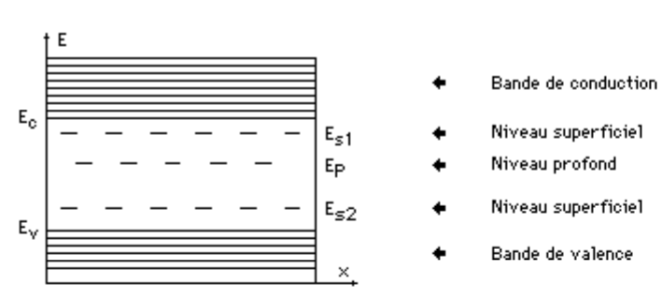
\includegraphics[width=0.6\textwidth]{ExN.PNG}
    \caption{Bandes d'énergie dans la bande interdite d'un cristal dopé}
    \label{fig:ExN}
\end{figure}
La présence de ces bandes extrinsèques influence les bandes d'énergie les plus proches (trous et électrons), ils influence de ce fait la conductivité du cristal.\\
La présence d'un niveau profond (proche du milieu) agit sur les deux bandes et facilite ainsi le transfert entre les bandes permises.

\subsubsection{Niveaux donneurs et accepteurs}
Le niveau d'énergie introduit par un atome est donné par la différence de potentiel du à l'ionisation.
\begin{equation}
P + \Delta E _ { D } \rightarrow P ^ { + } + ( - q )
\end{equation}
\begin{figure}
    \centering
    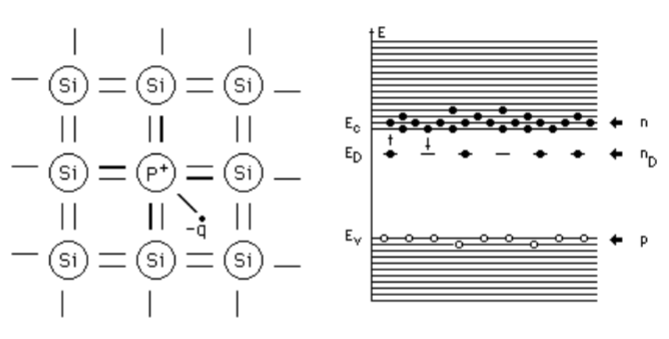
\includegraphics[width=0.7\textwidth]{Pdonne.PNG}
    \caption{Exemple de niveau d'énergie dans le cas d'un donneur P dans un cristal Si}
    \label{fig:Pexemple}
\end{figure}
\begin{figure}
    \centering
    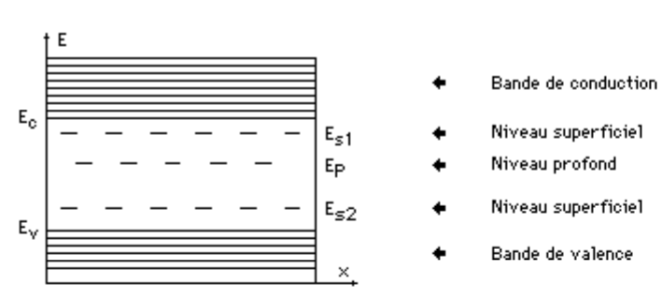
\includegraphics[width=0.7\textwidth]{ExN.PNG}
    \caption{Exemple de niveau d'énergie dans le cas d'un accepteur B dans un cristal Si}
    \label{fig:Nexemple}
\end{figure}
L'ionisation par un atome crée un réel excès en électrons/trous dans la bande de conduction/valence, alors que normalement le nombre de trous dans $E_v$ doit toujours être égal au nombre d'électrons dans $E_c$. Les niveaux introduits sont discret et localisé tant que la concentration en donneurs est faible. À partir d'un certain seuil de concentration les niveaux discret forment une bande d'énergie permise dans la bande interdite.

\subsubsection{Position énergétique des niveaux superficiels}
Soit un électron et un atome donneur ionisé. Puisque l'atome est intégré dans la maille comme si il s'agit d'un atome natif, on ne recalcule pas son effet sur les mailles, on ne prendra en compte que sa charge positive du à l'ionisation. On calcule donc l'équivalent d'un atome d'hydrogène ionisé localisé. On fera également l'approximation d'une masse effective scalaire $m ^ { * } = 0,5 \cdot m$. On calcule Schrödinger
\begin{gather}
V ( \overline { z } ) = - \frac { q ^ { 2 } } { 4 \pi \varepsilon _ { s } | \overline { z } | }\\
\left[ - \frac { \hbar ^ { 2 } \nabla^2 } { 2 m ^ { * } } - \frac { q ^ { 2 } } { 4 \pi \epsilon _ { s } | \overline { r } | } \right] \Phi ( \overline { r } ) = E \Phi ( \overline { r } ) \Longleftrightarrow E _ { n } = - \frac { m ^ { * } q ^ { 4 } } { 8 \left( \epsilon _ { s } h \right) ^ { 2 } } \frac { 1 } { n ^ { 2 } } , n = 1,2,3 , \dots
\end{gather}
L'ionisation complète de l'électron donne l'énergie $-E_1 = E_D$, il suffit de calculer l'énergie de la bande de conduction pour trouver $\Delta E_D = E_C-E_D$.\\
L'orbite de l'électron de niveau fondamental est donné par
\begin{equation}
n = 1 \Rightarrow r _ { o } = \frac{4 \pi \epsilon _ { s } h ^ { 2 } }{ m ^ { * } q ^ { 2 }}
\end{equation}
On remarque que le rayon est grand par rapport aux mailles du cristal, ça permet de justifier l'utilisation de la permittivité dans le calcul précédent malgré le fait que ce soit un phénomène macroscopique. Cela justifie également l'utilisation de la masse relative scalaire
\subsubsection{Fonction de distribution}
Nous devons maintenant calculer la distributions des porteurs au vu de ces nouveaux états énergétiques. Rappelons qu'un donneur émet un électron de spin déterminé mais un centre ionisé peut capturer une charge de spin quelconque, et une bande de conduction valence ne peut contenir que deux charges de spin opposé maximum.\\
Le nombre de possibilité de disposer $n_i$ électrons parmis $N_i$ états permis en tenant compte des spins est
\begin{equation}
W _ { i } = C_{n_i}^{2N_i} = \frac { \left( 2 N _ { i } \right) ! } { n _ { i } ! \left( 2 N _ { i } - n _ { i } \right) ! }
\end{equation}
Dans le cas des accepteurs, il y a $2N_D$ possibilités pour disposer le premier électrons, pour le second $N_D-1$
\begin{equation}
W_D=2 ^ { n } \cdot \frac { N _ { D } ! } { n _ { D } ! \left( N _ { D } - n _ { D } \right) ! }
\end{equation}
Le nombre total d'électrons dans les bandes permises et du niveau donneur est donc 
\begin{equation}
W = 2 ^ { n _ { D } } \cdot \frac { N _ { D } ! } { n _ { D } ! \left( N _ { D } - n _ { D } \right) ! } \cdot \prod _ { i } \frac { \left( 2 N _ { i } \right) ! } { n _ { i } ! \left( 2 N _ { i } - n _ { i } \right) ! }
\end{equation}
En calculant la suite 
\begin{gather}
    \frac { \partial } { \partial n _ { i } } ( \ln W - \alpha N - \beta E ) = 0 , \frac { \partial } { \partial n _ { D } } ( \ln W - \alpha N - \beta E ) = 0\\
    \ln A ! \approx A ( \ln A - 1 )\\
    \frac { n _ { i } } { 2 N _ { i } } = \frac { 1 } { 1 + e ^ { \alpha + \beta E _ { i } } } \quad,\quad \frac { n _ { D } } { N _ { D } } = \frac { 1 } { 1 + \frac { 1 } { 2 } e ^ { \alpha + \beta E _ { D } } }\\
    \beta = \frac { 1 } { k T }\quad,\quad\alpha = - \frac { \mu } { k T }
\end{gather}
Le nombre total d'électrons étant fixe à tout instants
\begin{equation}
N = \frac { N _ { D } } { 1 + \frac { 1 } { 2 } e ^ { \left( E _ { D } - \mu \right) / k T } } + \sum _ { i } \frac { 2 N _ { i } } { 1 + e ^ { \left( E _ { i } - \mu \right) / k T } }
\end{equation}
On tombe finalement sur la distribution de Fermi-Dirac pour les bandes permises, et sur la fonction de distribution suivante pour les centres donneurs
\begin{equation}
\frac { n _ { i } } { 2 N _ { i } } = f _ { F D } \left( E _ { i } \right) = \frac { 1 } { 1 + e ^ { \left( E _ { i } - \mu \right) / k T } }\quad,\quad\frac { n _ { D } } { N _ { D } } = f \left( E _ { D } \right) = \frac { 1 } { 1 + \frac { 1 } { 2 } e ^ { \left( E _ { D } - \mu \right) / k T } }
\end{equation}
On appelle le coefficient $1/2$ le facteur de dégénérescence du niveau donneur. Par raisonnement analogue on trouve la distribution d'électrons dans le cas de dopage accepteur
\begin{equation}
\frac { n _ { A } } { N _ { A } } = f \left( E _ { A } \right) = 1 - \frac { 1 } { 1 + \frac { 1 } { 2 } e ^ { \left( \mu - E _ { A } \right) / k T } } = \frac { 1 } { 1 + 2 e ^ { \left( E _ { A } - \mu \right) / k T } }
\end{equation}
avec un facteur de dégénérescence égal à $2$.\\
On définie ce qu'on appellera l'énergie effective, elle permet d'avoir une même distribution dans les trois cas respectivement intrinsèque, donneur, et accepteur
\begin{equation}
E _ { t } = \left\{ \begin{array} { r } { E _ { i } } \\ { E _ { D } - k T \log 2 } \\ { E _ { A } + k T \log 2 } \end{array} \right.
\end{equation}

\subsubsection{Semiconducteurs non-dégénérées et dégénérées}
Nous connaissons la concentration d'équilibre d'un semiconducteur
\begin{equation}
n = 2 \int _ { E _ { c } } ^ { E _ { M c } } N _ { c } ( E ) f _ { F D } ( E ) d E
\end{equation}
Le potentiel d'équilibre est appelé niveau de Fermi et est noté $\mu = E_F$. Le niveau de Fermi est une fonction de la température et du dopage. La substitution entraine une erreur de moins de 5\% tant que $E _ { c } - E _ { F } > 3 k T$. On remplace ainsi la fonction de Fermi-Dirac 
\begin{equation}
n = 2 \int _ { E _ { c } } ^ { E _ { M c } } N _ { c } ( E ) f _ { F D } ( E ) d E \quad,\quad p = 2 \int _ { E _ { m v } } ^ { E _ { v } } N _ { v } ( E ) \left[ 1 - f _ { F D } ( E ) \right] d E
\end{equation}
par celle de Maxwelle-Boltzmann
\begin{equation}
n = 2 \int _ { E _ { c } } ^ { E _ { M c } } N _ { c } ( E ) e ^ { - \left( E - E _ { F } \right) / k T } d E \quad,\quad p = 2 \int _ { E _ { m v } } ^ { E _ { v } } N _ { v } ( E ) e ^ { \left( E - E _ { F } \right) / k T } d E
\end{equation}
Si le niveau de Fermi se trouve à moins de $3kT$ des limites des bandes de conduction ou de valence, le conducteur est dégénéré car les bandes intrinsèques et extrinsèques se superposent/sont très proches. Le semiconducteur se comporte alors comme un métal. 

\subsubsection{Semiconducteur non-dégénéré : concentrations
d’équilibre}
Il est temps de résoudre l'intégrale de la densité d'états, on reprend les expressions précédentes et on intègre jusqu'à l'infinie car la valeur de l'intégrale est proche de nulle pour des valeurs supérieures à $E_{C/V}$
\begin{gather}
N _ { c } ( E ) = \frac { \sqrt { m _ { c } ^ { 3 } \left( E - E _ { c } \right) } } { \sqrt { 2 } \pi ^ { 2 } h ^ { 3 } } \quad,\quad u = \frac{E - E _ { c }}{kT}\quad,\quad \int _ { 0 } ^ { \infty } \sqrt { u } e ^ { - u } d u = \frac { \sqrt { \pi } } { 2 }\\
n = \frac { \sqrt { 2 \left( m _ { c } k T \right) ^ { 3 } } } { \pi ^ { 2 } h ^ { 3 } } \cdot e ^ { - \left( E _ { c } - E _ { F } \right) / k T } \cdot \int _ { 0 } ^ { \infty } \sqrt { u } e ^ { - u } d u\\
n = N _ { c } e ^ { \left( E _ { F } - E _ { c } \right) / k T }\quad,\quad N _ { c } = \frac { 2 \left( 2 \pi m _ { c } k T \right) ^ { 3 / 2 } } { h ^ { 3 } }
\end{gather}
même raisonnement pour $p$
\begin{gather}
    N _ { v } ( E ) = \frac { \sqrt { m _ { v } ^ { 3 } \left( E _ { v } - E \right) } } { \sqrt { 2 } \pi ^ { 2 } \hbar ^ { 3 } }\\
    p = N _ { v } e ^ { \left( E _ { v } - E _ { F } \right) / k T }\quad,\quad N _ { v } = \frac { 2 \left( 2 \pi m _ { v } k T \right) ^ { 3 / 2 } } { h ^ { 3 } }
\end{gather}
On tentera maintenant de définir $E_i$ pour faciliter les calcules à l'avenir. Soit le produit des porteurs
\begin{equation}
n . p = N _ { c } N _ { v } e ^ { - \left( E _ { c } - E _ { v } \right) / k T }
\end{equation}
Celui-ci est indépendant du niveau de Fermi et du dopage, c'est un paramètre intrinsèque au matériau considéré
\begin{equation}
\left[ n _ { i } ( T ) \right] ^ { 2 } = n . p = \frac { 4 } { h ^ { 6 } } ( 2 \pi k T ) ^ { 3 } \left( m _ { c } m _ { v } \right) ^ { 3 / 2 } e ^ { - \left( E _ { c } - E _ { v } \right) / k T }
\end{equation}
Dans le cas d'un conducteur intrinsèque le nombre d'électrons est toujours égal au nombre de trous, $n = p = n _ { i }$. Seul la valeur de $E_g = E _ { c } - E _ { v }$ peut varier avec la température.

\begin{figure}
    \centering
    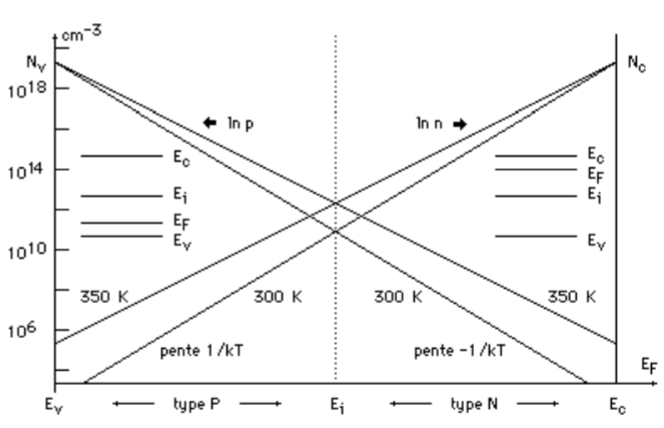
\includegraphics[width=0.5\textwidth]{porteursD.PNG}
    \caption{Diagramme des porteurs en fonction du niveau d'énergie du niveau de Fermi, niveau intrinsèque comme référence}
    \label{fig:PorteursD}
\end{figure}

\subsubsection{Niveau de Fermi d'un cristal intrinsèque}
Il n'y a pas d'excès de porteur donc
\begin{equation}
n = p = n _ { i } = N _ { c } e ^ { \left( E _ { i } - E _ { c } \right) / k T } = N _ { v } e ^ { \left( E _ { v } - E _ { i } \right) / k T }
\end{equation}
Il suffit de mettre en évidence $E_i$
\begin{equation}
E _ { i } = \frac { 1 } { 2 } \left( E _ { c } + E _ { v } \right) \left(\frac { 3 } { 2 } k T \ln \left( + \frac { m _ { v } } { m _ { c } } \right) \approx 0\right)
\end{equation}
\subsubsection{Niveau de Fermi d’un semiconducteur homogène dopé}
Soit un semi conducteur dopé en donneurs et en accepteurs de manière homogène. Nous savons que la somme des porteurs est nulle par la neutralité électrique.
\begin{equation}
p + N _ { D } ^ { + } = n + N _ { A } ^ { - }
\end{equation}
Calculons le nombre de porteurs ionisé en fonction du niveau de fermi
\begin{gather}
N _ { D } ^ { + } = \left[ 1 - \frac { 1 } { 1 + \frac { 1 } { 2 } e ^ { \left( E _ { D } - E _ { F } \right) / k T } } \right] N _ { D } = \frac { N _ { D } } { 1 + 2 e ^ { \left( E _ { F } - E _ { D } \right) / k T } }\\
N _ { A } ^ { - } = \frac { N _ { A } } { 1 + 2 e ^ { \left( E _ { A } - E _ { F } \right) / k T } }
\end{gather}
En mettant tout ça dans l'équation de neutralité électrique on obtient 
\begin{equation}
N _ { v } e ^ { \left( E _ { v } - E _ { F } \right) / k T } + \frac { N _ { D } } { 1 + 2 e ^ { \left( E _ { F } - E _ { D } \right) / k T } } = N _ { c } e ^ { \left( E _ { F } - E _ { c } \right) / k T } + \frac { N _ { A } } { 1 + 2 e ^ { \left( E _ { A } - E _ { F } \right) / k T } }
\end{equation}
On préfère travailler en échelle logarithmique pour en faire un permière analyse graphique \href{fig:NFermi}{Figure \ref{fig:NFermi}}. $N_D$ le nombre de donneurs, $N_C$ le nombre d'électrons, $N_v$ le nombre de trous, $N_A$ le nombre d'accepteurs
\begin{figure}[H]
    \centering
    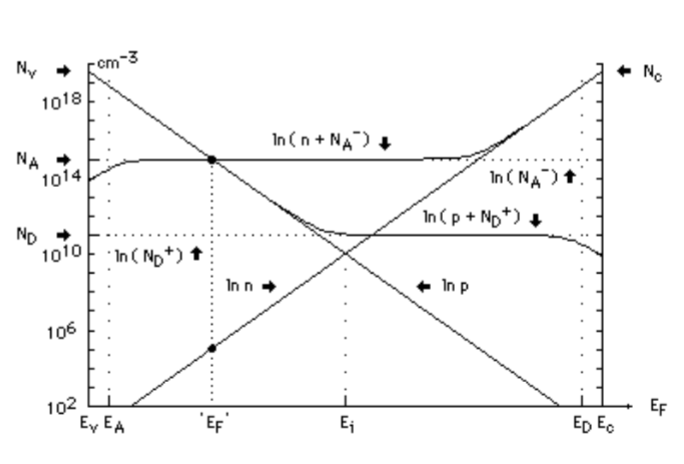
\includegraphics[width=0.6\textwidth]{FermiG.PNG}
    \caption{Analyse graphique des concentration de porteurs en fonction du niceau de Fermi}
    \label{fig:NFermi}
\end{figure}
On remarque immédiatement graphiquement que, dans ces ordres de grandeur, les approximations sont valables
\begin{gather}
N _ { A } ^ { - } = N _ { A } \quad,\quad p = N _ { A }\quad,\quad n = \frac { n _ { i } ^ { 2 } } { N _ { A } }
\end{gather}
On trouve ainsi facilement 
\begin{equation}
E _ { F } = E _ { v } + k T \ln \left( \frac { N _ { v } } { N _ { A } } \right) = E _ { i } - k T \ln \left( \frac { N _ { A } } { n _ { i } } \right)
\end{equation}
On en conclu que en toutes généralitées, les équations suivantes sont valables\\
si $N _ { A } >> N _ { D }$ :
\begin{gather}
N _ { A } ^ { - } = N _ { A }\\
p = N _ { A }\quad,\quad n = n _ { i / N _ { A } } ^ { 2 }\\
E _ { F } = E _ { r } + k T \ln \frac { N _ { v } } { N _ { A } } = E _ { i } + k T \ln \frac { n _ { i } } { N _ { A } }\\
\end{gather}
Si $N _ { D } >> N _ { A }$ :
\begin{gather}
N _ { D } ^ { + } = N _ { D }\\
n = N _ { D }\quad,\quad p = n _ { i } ^ { 2 } / N _ { D }\\
E _ { F } = E _ { c } - k T \ln \frac { N _ { c } } { N _ { D } } = E _ { i } + k T \ln \frac { N _ { D } } { n_ { i } }
\end{gather}
Bien sûr, ces formules ne sont valables que si le semiconducteur n'est pas dégénéré (assimilable à un métal), auquel cas il faudrait laisser tomber l'approximation d'utiliser $f_{MB}$ à la place $f_{FD}$.\\
On distingue encore deux cas particulier \href{fig:Tdiag}{Figure \ref{fig:Tdiag}}:\\
\textbf{Basse Température :} Les pentes de $p$ et $n$ sont très abruptes, l'intersection se trouve en dessous du niveau extrinsèque introduit. On est en dehors de l'écart $3kT$ et le semiconducteur est dégénéré.\\
\textbf{Haute Température :} Le niveau de $n_i(T)$ est très haut et prime sur le dopage, on retrouve donc $n=p=n_i$.\\
\begin{figure}
    \centering
    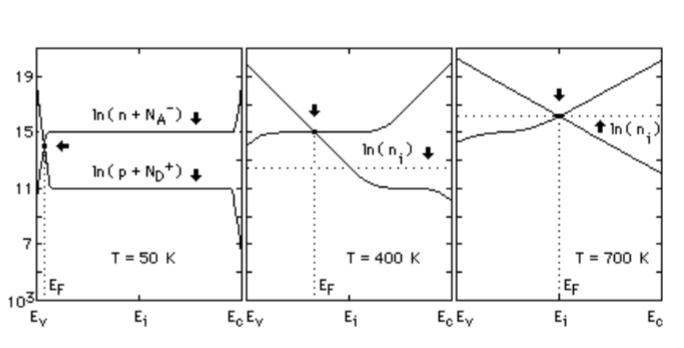
\includegraphics[width=0.7\textwidth]{Tdiag.PNG}
    \caption{Densité de porteur en fonction du niveau de Fermi à différentes T}
    \label{fig:Tdiag}
\end{figure}

\section{Vibration de Réseau}
\subsection{Vibration d'une chaîne unidimensionnelle}
Soit une chaîne de longueur $aN$, avec les atomes aux positions 
\begin{equation}
x_n = n\cdot a\quad n = 1,2,\dots,N
\end{equation}
auquel on associe une déviation de position du à la vibration 
\begin{equation}
y _ { n } = f(x_n) \quad n = 1,2 , \ldots , N
\end{equation}
On applique une force sur l'atome $n$ uqi le fera se déplacer et entrainera les atomes voisins $n - 1 \text { et } n + 1$.
\begin{equation}
F _ { n } = F _ { n } \left( y _ { n } - y _ { n - 1 } , y _ { n } - y _ { n + 1 } \right)
\end{equation}
On ne considère que les termes linéaires pour développer, avec $\beta$ la constante de force
\begin{equation}
\begin{array} { l } { F _ { n } = - \beta \left( y _ { n } - y _ { n - 1 } \right) - \beta \left( y _ { n } - y _ { n + 1 } \right) } \\ { F _ { n } = - \beta \left( 2 y _ { n } - y _ { n - 1 } - y _ { n + 1 } \right) } \end{array}
\end{equation}
On développe l'équation classique d'un mouvent oscillatoire
\begin{gather}
M \frac { d ^ { 2 } y _ { n } } { d t ^ { 2 } } = - \beta \left( 2 y _ { n } - y _ { n - 1 } - y _ { n + 1 } \right)
\end{gather}
Le cristal étant symétrique, il s'agit d'une fonciton de Bloch
\begin{equation}
y _ { n } ( t ) = Q _ { q } ( t ) e ^ { i q ( n a ) } \Rightarrow M \frac { d ^ { 2 } Q _ { q } ( t ) } { d t ^ { 2 } } = - 2 \beta [ 1 - \cos ( q a ) ] Q _ { q } ( t )
\end{equation}
On trouve finalement comme solution un oscillateur harmonique dépendant du nombre d'onde $q$, ainsi que la relation de dispersioni associée
\begin{equation}
Q _ { q } ( t ) = A e ^ { - i \omega ( a ) t } , \omega \geq 0\quad,\quad \omega ( q ) = 2 \sqrt { \frac { \beta } { M } } \left| \sin \left( \frac { q a } { 2 } \right) \right| = \omega _ { c } \left| \sin \left( \frac { q a } { 2 } \right) \right|
\end{equation}
L'expression complète est 
\begin{equation}
y _ { n } ( t ) = A e ^ { i [ q ( n a ) - \omega ( q ) t ] }
\end{equation}
\begin{figure}
    \centering
    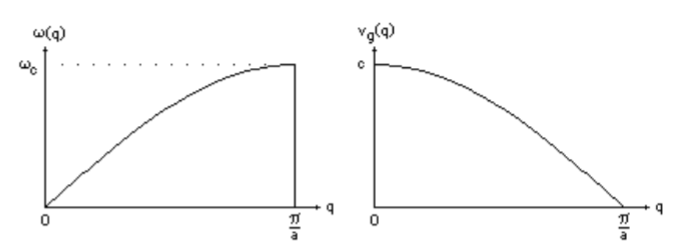
\includegraphics[width=0.6\textwidth]{Pulse.PNG}
    \caption{Pulsation et amplitude dans la zone de Brioullin}
    \label{fig:pulse}
\end{figure}
On procède comme précédemment pour trouver la vitesse de groupe
\begin{gather}
y _ { n } ( t ) = \int _ { - \pi / a } ^ { \pi / a } A ( q ) e ^ { i [ q ( n a ) - \omega ( a ) t ] } d q\\
y _ { n } ( x ; t ) = \int _ { - \pi / a } ^ { \pi / a } A ( q ) e ^ { i [ q x - \omega ( a ) t ] } d q\\
v _ { g } ( q ) = \frac { d \omega } { d q } = \frac { 1 } { 2 } a \omega _ { c } \left| \cos \left( \frac { q a } { 2 } \right) \right| = c \left| \cos \left( \frac { q a } { 2 } \right) \right|
\end{gather}
Le cristal à une fréquence maximale et une vitesse maximale proche $q=0$
\begin{equation}
\omega ( q ) = c q \quad, \quad v _ { g } ( q ) = c = a \omega _ { c } / 2
\end{equation}
On prend maintenant également en compte les dimensions finies du cristal, soit la longueur $L=aN$
\begin{gather}
y _ { n } ( t ) = y _ { n + N } ( t )\\
e ^ { i q N a } = 1\\
q = \pm \frac { 2 \pi } { N a } , \pm \frac { 4 \pi } { N a } , \ldots , \pm \frac { \pi } { a }\\
y _ { n } ( t ) = Q _ { q } ( t ) e ^ { i q ( n a ) }
\end{gather}
De part la quantification du nombre $q$, du fait qu'il ne peut être nulle, on trouve que les pulsations permises sont données par

\begin{equation}
\omega ( q ) = \frac { 2 c } { a } \left| \sin \left( \frac { q a } { 2 } \right) \right|
\end{equation}
L'équation du mouvement de l'oscillateur harmonique est donné par 
\begin{equation}
\frac { d ^ { 2 } Q _ { q } ( t ) } { d t ^ { 2 } } + \omega ^ { 2 } ( q ) Q _ { q } ( t ) = 0
\end{equation}
\subsection{Étude Quantique}
On repart de l'équation de Schrödinger pour un ensemble de $N-1$ oscillateurs harmoniques
\begin{equation}
\sum _ { 1 } ^ { N - 1 } \left[ - \frac { \hbar ^ { 2 } } { 2 M } \frac { d ^ { 2 } } { d Q _ { q } ^ { 2 } } + \frac { 1 } { 2 } M \omega ^ { 2 } ( q ) Q _ { q } ^ { 2 } ( t ) \right] \Phi = E \Phi
\end{equation}
On fera l'étude sur les oscillateur indépendemment par séparation de variable
\begin{gather}
\Phi = \prod _ { 1 } ^ { N - 1 } \Phi _ { q } \left( Q _ { q } \right) \quad , \quad E = \sum _ { 1 } ^ { N - 1 } E _ { q }\\
\left[ - \frac { \hbar ^ { 2 } } { 2 M } \frac { d ^ { 2 } } { d Q _ { q } ^ { 2 } } + \frac { 1 } { 2 } M \omega ^ { 2 } ( q ) Q _ { q } ^ { 2 } ( t ) \right] \Phi _ { q } \left( Q _ { q } \right) = E _ { q } \Phi _ { q } \left( Q _ { q } \right)
\end{gather}
L'énergie des oscillateurs harmoniques $\Phi_q(Q_q)$ de pulsation $\omega(q)$ et d'énergie $E_q$ s'exprime comme suit
\begin{equation}
E _ { q } = \left( n _ { q } + \frac { 1 } { 2 } \right) \hbar \omega ( q ) \quad , \quad n _ { q } = 0,1,2,3 , \dots
\end{equation}
et donc l'énergie total est
\begin{equation}
E _ { 0 } = \frac { \hbar } { 2 } \sum _ { 1 } ^ { N - 1 } \omega ( q ) = \frac { c \hbar } { a } \sum _ { 1 } ^ { N - 1 } \left| \sin \left( \frac { q a } { 2 } \right) \right|\quad,\quad E - E _ { 0 } = \sum _ { 1 } ^ { N - 1 } n _ { q } \hbar \omega ( q )
\end{equation}
En approximant pas une intégrale on obtient le résultat
\begin{equation}
E _ { 0 } = \frac { 2 N c h } { \pi a } = \frac { N \omega _ { c } h } { \pi }
\end{equation}
L'interprétation de ce phénomène est :  il existe des particules nommées phonons, d'énergie $E - E _ { 0 }$, $N - 1$ niveaux permis $\hbar \omega ( q )$, $n _ { q }$ quanta qur le niveau de vibration $\hbar \omega ( q )$, on peut donc leur trouver une distribution 
\begin{equation}
n _ { q } = \frac { 1 } { e ^ { \hbar \omega ( q ) / k T } - 1 }
\end{equation}
donc l'énergie totale est 
\begin{gather}
E = E _ { 0 } + \sum _ { 1 } ^ { N - 1 } \frac { \hbar \omega ( q ) } { e ^ { \hbar \omega ( q ) / k T } - 1 }\\
E = E _ { 0 } + \frac { 2 N } { \pi } \int _ { 0 } ^ { \omega _ { c } } \frac { \hbar \omega } { e ^ { \hbar \omega / k T } - 1 } \cdot \frac { d \omega } { \sqrt { \omega _ { c } ^ { 2 } - \omega ^ { 2 } } }
\end{gather}
à haute température l'expression devient
\begin{equation}
E = E _ { 0 } + N k T = N \left( k T + \frac { 2 c h } { \pi a } \right)
\end{equation}
et si $E_0$ est négligeable
\begin{equation}
E = N . k T
\end{equation}
Le but de toute cette démonstration était de retomber sur le résultat suivant
\begin{equation}
E_{3D} = 3N . k T
\end{equation}
qui est exactement le même résultat que pour les vibrations d'un ensemble de particules libres, on peut ainsi utiliser le concepte de phonons pour étudier les interaction entre le cristal et les électrons comme si les deux étaitent des gaz.\\
L'impulsion d'un phonon est donnée par
\begin{equation}
p _ { q } = \frac { \hbar \omega ( q ) } { v _ { g } ( q ) }
\end{equation}
\subsection{Cas d'une chaîne diatomique}
On travaille avec une chaîne à atomes intermittents, les équations sont les mêmes que précédemment 
\begin{gather}
\begin{array} { l } { M _ { 1 } \frac { d ^ { 2 } u _ { n } } { d t ^ { 2 } } = - \beta \left( 2 u _ { n } - y _ { n } - y _ { n - 1 } \right) } \\ { M _ { 2 } \frac { d ^ { 2 } y _ { n } } { d t ^ { 2 } } = - \beta \left( 2 y _ { n } - u _ { n } - u _ { n + 1 } \right) } \end{array}\\
\begin{array} { l } { u _ { n } ( t ) = A e ^ { i q ( 2 n ) a } . e ^ { - i \omega t } } \\ { y _ { n } ( t ) = B e ^ { i q ( 2 n + 1 ) a } \cdot e ^ { - i \omega t } } \end{array}\\
\begin{array} { l } { M _ { 1 } \omega ^ { 2 } A = 2 \beta [ A - B \cos ( q a ) ] } \\ { M _ { 2 } \omega ^ { 2 } B = 2 \beta [ B - A \cos ( q a ) ] } \end{array}\\
\end{gather}
On trouves grâce au déterminant nulle la relation de dispersion (ici $M_1<M_2$)
\begin{equation}
\omega _ { \pm } ( q ) = \sqrt { \beta } \sqrt { \frac { 1 } { M _ { 1 } } + \frac { 1 } { M _ { 2 } } \pm \sqrt { \left( \frac { 1 } { M _ { 1 } } + \frac { 1 } { M _ { 2 } } \right) ^ { 2 } - \frac { 4 \sin ^ { 2 } ( q a ) } { M _ { 1 } M _ { 2 } } } }
\end{equation}
On distingue deux branches de pulsations $\omega_+$ et $\omega_-$, les quanta de fréquences hautes sont appelées phonons optiques, et les fréquences basses phonons accoustiques. Ces deux fréquences sont séparés pas une bande interdite lié aux masses $M_1$ et $M_2$.  
On détermine les amplitudes $A$ et $B$ par
\begin{equation}
\frac { B } { A } = \frac { y _ { n } } { u _ { n } } e ^ { - i q a } = - \frac { M _ { 1 } - M _ { 2 } \pm \sqrt { \left( M _ { 1 } + M _ { 2 } \right) ^ { 2 } - 4 M _ { 1 } M _ { 2 } \sin ^ { 2 } ( q a ) } } { 2 M _ { 2 } \cos ( q a ) }
\end{equation}
\section{Équation de transport}
L'équation de transport est la base de l'étude des courant, car on assimilera le réseau et ses vibrations à des phonons et les électrons à un gaz d'une énergie précise.
\subsection{Collision entre électrons et phonons}
Soit un électrons dans un cristal parfait
\begin{gather}
\Psi ( \overline { r } , t ) = \sum _ { Z B } A ( \overline { k } ) u _ { \overline { k } } ( \overline { r } ) e ^ { i \left[ \overline { k } \cdot \overline { r } - E _ { n } ( \overline { k } ) t / \hbar \right] }\\
\overline { \nu } _ { g } ( \overline { k } ) = \frac { 1 } { \hbar } \operatorname { grad } _ { \overline { k } } E _ { n } ( \overline { k } )
\end{gather}
Les collisions avec le réseau de cet électron provoque son déplacement. Dans le cas d'un gaz d'électrons il s'agit de diffusion, car l'absence d'électrons dans un espace signifie moins de collisions venant de celui-ci, provoquant une delta de déplacement en moyenne sur la trajectoire aléatoire de l'électron. Dans le cas d'un champ électrique, il y a une force agissant sur l'électron, provoquant un delta de dérive se dégageant de son mouvement aléatoire.
\begin{figure}
    \centering
    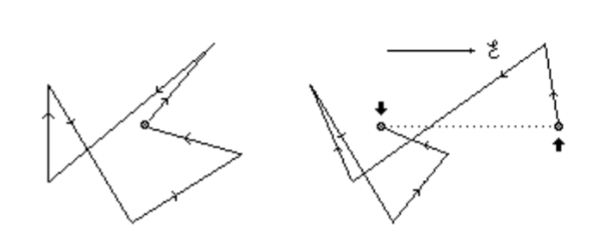
\includegraphics[width=0.5\textwidth]{DeltaCollision.PNG}
    \caption{Déplacement d'une particule sous l'influence d'un champ}
    \label{fig:Ddepl}
\end{figure}
\subsection{Vitesse de dérive dans un champ électrique}
Soit le temps moyen entre deux collisions $\tau_n$, considéré isotrope (direction de collision aléatoire). Soit le nombre d'électrons subissant une collision au temps $t_0$ vaut $n(t_0)$. On commence l'observation des collision à partir de ce moment là. À l'instant $t$, $n(t)$ électrons effectuent une collsion, réduisant de $dn$ le nombre d'électrons n'ayant pas fait de collision.
\begin{equation}
d n = - \frac { n ( t ) } { \tau _ { n } } d t \quad ( < 0 )
\end{equation}
Dont la solution est 
\begin{equation}
n ( t ) = n \left( t _ { o } \right) e ^ { - \left( t - t _ { o } \right) / \tau _ { n } }
\end{equation}
Il y a donc $-dn$ collisions entre $t-t_0$, on cherche la moyen de temps entre collisions donc
\begin{equation}
\frac { 1 } { n \left( t _ { o } \right) } \int _ { n \left( t _ { o } \right) } ^ { 0 } \left( t - t _ { o } \right) ( - d n ) = \frac { 1 } { \tau _ { n } n \left( t _ { o } \right) } \int _ { t _ { o } } ^ { \infty } \left( t - t _ { o } \right) n \left( t _ { o } \right) e ^ { - \left( t - t _ { o } \right) / \tau _ { n } } d t = \tau _ { n }
\end{equation}
Étudions maintenant l'influence du champ électrique, soit l'équation du mouvement
\begin{equation}
m _ { n } ^ { * } \frac { d \overline { v } } { d t } = - q \overline { \mathcal { E } }
\end{equation}
La vitesse en trois dimensions d'un électron n'ayant pas subit de nouvelle collision est 
\begin{equation}
\overline { v } ( t ) = \overline { v } \left( t _ { o } \right) - \frac { q \overline { \mathcal { E } } } { m _ { n } ^ { * } } \left( t - t _ { o } \right)
\end{equation}
On utilise cette relation sur le $n(t_0)$ électrons libres n'ayant pas subit de collision et se déplaçant selon le champ électrique
\begin{gather}
\overline { v } _ { d , n } = \frac { 1 } { n \left( t _ { o } \right) } \int _ { n \left( t _ { o } \right) } ^ { 0 } \frac { - q \overline { \mathcal { E } } } { m _ { n } ^ { * } } \left( t - t _ { o } \right) ( - d n )\\
\overline { v } _ { d , n } = \frac { q \overline { \mathcal { E } } } { m _ { n } ^ { * } \tau _ { n } } \int _ { t _ { o } } ^ { \infty } \left( t - t _ { o } \right) e ^ { - \left( t - t _ { o } \right) / \tau _ { n } } d t
\end{gather}
On utilise à nouveau le temps moyen pour finalement trouver
\begin{equation}
\overline { v } _ { d , n } = - \mu _ { n } \overline { \mathcal { E } } \quad\text{avec}\quad \mu _ { n } = \frac { q \tau _ { n } } { m _ { n } ^ { * } }
\end{equation}
Par raisonnement analoque on trouve la vitesse moyenne de dérive des trous
\begin{equation}
\overline { v } _ { d , p } = + \mu _ { p } \overline { \mathcal { E } } \quad\text{avec}\quad \mu _ { p } = \frac { q \tau _ { p } } { m _ { p } ^ { * } }
\end{equation}
Nous avons fait l'hypothèse que les collisisons sont isotropes, c'est le cas uniquement pour les interactions avec le réseau. Dans le cas d'une impureté ionisé, la collision est une déviation de trajectoire (collision de Rutherford).\\
Nous faisons également l'hypothèse que le temps de libre parcours moyen est indépendant de l'énergie des porteurs, en pratique ce n'est pas le cas et notre modèle ne fait que la moyenne de cette énergie.\\
On admet les collsions isotropes et donc la masse effective scalaire ce qui n'est pas le cas en toutes généralités. La mobilité est donc un tenseur, néanmoins la symétrie du réseau peut rendre le tenseur scalaire par exemple dans le cas de symétrie cubique.
\subsection{Étude de la mobilité}
Le mobilité est composée de deux contributions, les collision avec le réseau $\mu_r$ et les collision avec les impuretés chargées $\mu_i$.
\begin{equation}
    \mu _ { r } = \frac { A } { T ^ { 3 / 2 } }\quad,\quad\mu _ { i } = \frac { B T ^ { 3 / 2 } } { N }
\end{equation}
La mobilité totale est donnée par la relation
\begin{equation}
\frac { 1 } { \mu } = \frac { 1 } { \mu _ { r } } + \frac { 1 } { \mu _ { i } } = \frac{T^{3/2}}{A}+\frac{N}{BT^{3/2}}
\end{equation}
\textbf{N faible :} Les collisions avec le réseau sont prépondérantes, diminue avec $T$.\\
\textbf{N grands :} Les cas de haute et basse températures doivent être analysés séparément. À basse température les collisions avec les charges dominent, à haute température les collisions avec le réseau dominent.\\
Le modèle que nous avons ici construit n'est pas complet, il ne prend pas en compte les interactions entre porteurs libres, les
collisions avec les impuretés neutres et les collisions avec les défauts
cristallins.
\subsubsection{Densité de courant}
La densité de courant de dérive est le courant donné par l'effet d'un champ électrique sur les électrons, il s'exprime respectivement pour les électrons et les trous
\begin{equation}
\overline { J } _ { n } = - q n \overline { v } _ { d , n } = + q n \mu _ { n } \overline { \mathcal { E } }\quad,\quad \overline { J } _ { p } = + q p \overline { \nu } _ { d , p } = + q p \mu _ { p } \overline { \mathcal { E } }
\end{equation}
La résistivité $\rho$ et la conductivité $\sigma$ sont donnés par
\begin{equation}
\rho = \frac { 1 } { \sigma }\quad,\quad \sigma = q \left( n \mu _ { n } + p \mu _ { p } \right)
\end{equation}

La mobilité des porteurs dépend du champ électrique appliqué et suit une loi asymptotique, à partir de $10^3,10^4V$ le courant devient constant

\begin{equation}
\mu = \frac { \mu _ { o } } { \left[ 1 + \left( | \overline { E } | / \left| \overline { \mathcal { E } } _ { c } \right| \right) ^ { \beta } \right] ^ { 1 / \beta } }
\end{equation}

avec $\overline { \mathcal { E } } _ { c }$ le champ caractéristique constant. Ce phénomène est du aux collisions. L'énergie cinétique des porteurs est entièrement transféré au réseau cristallin lors des collisions. À haute température l'échange est partiel et les porteurs conservent leur énergie. Il faut alors prendre en compte les interactions entre porteurs pour calculer la mobilité.\\
\subsubsection{Effet Hall}
Effet selon lequel, appliquer un champ électrique longitudinal et un champ magnétique vertical produit une force électromotrice latérale proportionnel au matériau et aux champ \href{fig:Hall}{Figure \ref{fig:Hall}}. 
\begin{figure}{H}
    \centering
    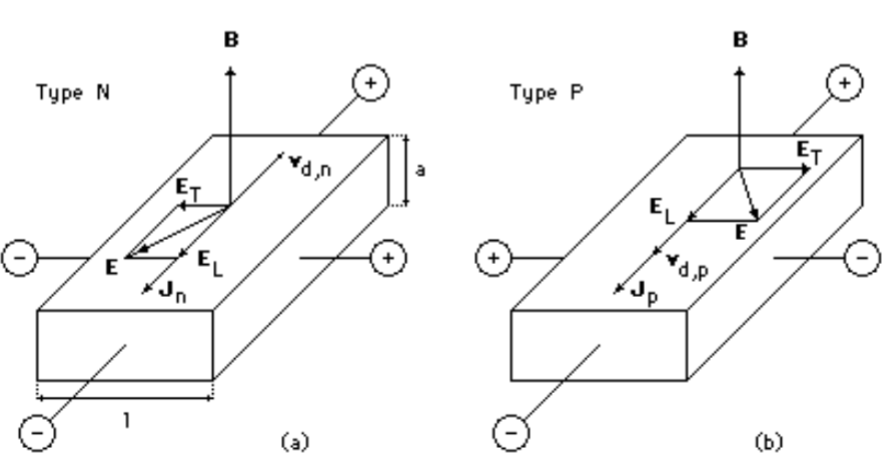
\includegraphics[width=0.7\textwidth]{EHall.PNG}
    \caption{Illustration de l'effet Hall dans le cas d'un semiconducteur N et P}
    \label{fig:Hall}
\end{figure}

En repartant de la densité de courant
\begin{gather}
\overline { J } _ { n } = q n \mu _ { n } \overline { \mathcal { E } } _ { L } = - q n \overline { v } _ { d , n }
\end{gather}
Par l'effet de la force de Lorentz, chaque électron $n$ se déplaçant longitudinalement dérive également latéralement, provoquant à son tour une distribution inégal de porteur qui engendre unchamp transverse $\mathcal{E}_t$.
\begin{equation}
\overline { \mathcal { E } } _ { T } = \overline { B } \otimes \overline { \boldsymbol { v } } _ { d , n } = - \frac { 1 } { q n } \left( \overline { B } \otimes \overline { J } _ { n } \right) = - \mu _ { n } \left( \overline { B } \otimes \overline { \mathcal { E } } _ { L } \right)
\end{equation}
La tension et le courant sont définit par les dimensions
\begin{equation}
V _ { H } = l . \overline { | \mathcal { E } } _ { T } |\quad,\quad \overline { I } = ( a l ) \overline { J } _ { n }
\end{equation}
On cherche le coefficient de Hall définit comme suit dans le cas ou le champ magnétique et le courant sont perpendiculaires
\begin{equation}
R _ { H , n } = \frac { a V _ { H } } { | \overline { I } | \cdot | \overline { B } | }= \frac { \left| \overline { \mathcal { E } } _ { T } \right| } { \left| \overline { J } _ { n } \right| \cdot | \overline { B } | } = - \frac { 1 } { q n }
\end{equation}
Soit la conductivité électrique du semiconducteur
\begin{equation}
\sigma _ { n } = q n \mu _ { n } \quad\Rightarrow\quad R _ { H , n } \cdot \sigma _ { n } = - \mu _ { n }
\end{equation}
De manière similaire pour un conducteur de type P
\begin{equation}
R _ { H , p } = + \frac { 1 } { q p } , \sigma _ { p } = q p \mu _ { p } , \quad R _ { H , p . \sigma _ { p } } = + \mu _ { p }
\end{equation}
La valeur de la constante de temps n'est pas indépendante de l'énergie. Dans le cas d'un métal, il faut prendre en compte la valeur du potentiel chimique $\mu$ lors du calcul de de $\tau(\mu)$. Dans le cas d'un semiconducteur, la différence est linéaire, il suffit donc juste d'appliquerun facteur de correction $r$.
\begin{equation}
R _ { H , n } = - \frac { r } { q n } \quad , \quad R _ { H , p } = + \frac { r } { q p }
\end{equation}

\section{Dopage non-homogène}
\subsection{Phénomènes à l'oeuvre}
La jonction analysée ici est extrêmement abrupte, bien que ce ne soit pas un cas réel car celle-ci doit être graduelle. Ici le contact se fait entre des matériaux de type P et N. Leurs niveaux de Fermi sont donc différents.\\
Le gradient de charges abrupte fait migrer les électrons et trous vers la jonction. Des deux cotés, les zones sont dépeuplés de leurs majoritaires ce qui crée un champ électrique entre les zones dépeuplées et les majoritaires, les empêchant ainsi de migrer. Il se forme ainsi un équilibre thermodynamique.\\
À l'équilibre, le potentiel interne doit être égal au potentiel de lla différence des niveaux de 
Fermi
\begin{equation}
q \Phi _ { 0 } = E _ { F n } - E _ { F p }
\end{equation}
On devra tout d'abord décrire le comportement d'un électron soumis au potentiel et au gradient de diffusion. Soit l'énergie d'un électron près du minimum de la bande de conduction 
\begin{equation}
E _ { c } ( k ) = E _ { c o } + \frac { \hbar ^ { 2 } k ^ { 2 } } { 2 m ^ { * } }
\end{equation}
Sa vitesse est 
\begin{equation}
v ( k ) = \frac { 1 } { h } \frac { d E _ { c } } { d k } = \frac { \hbar k } { m ^ { * } }
\end{equation}
On réécrit l'énergie
\begin{equation}
E _ { c } ( k ) = E _ { c o } + \frac { 1 } { 2 } m ^ { * } v ^ { 2 }
\end{equation}
On introduit le terme de perturbation dans l'équation de Schrödinger
\begin{equation}
\left[ - \frac { \hbar ^ { 2 } } { 2 m ^ { * } } \frac { d ^ { 2 } } { d x ^ { 2 } } + E _ { c o } - q \Phi ( x ) \right] \Psi ( x ) = E \Psi ( x )
\end{equation}
En travaillant sur des petits intervalles $dj$ pour approximer les contributions de chaque particule, on peut trouver l'énergie $E$
\begin{gather}
\left( - \frac { \hbar ^ { 2 } } { 2 m ^ { * } } \frac { d ^ { 2 } } { d x ^ { 2 } } + E _ { c o } - q \Phi _ { j } \right) \Psi _ { j } ( x ) = E \Psi _ { j } ( x )\\
\Psi _ { j } ( x ) = A _ { j } e ^ { i k j } x + B _ { j } e ^ { - i k _ { j } x }\\
E = E _ { c o } - q \Phi _ { j } + \frac { \hbar ^ { 2 } k _ { j } ^ { 2 } } { 2 m ^ { * } }
\end{gather}
Il suffit alors d'imposer la continuité entre les régions $\left( x _ { j - 1 } , x _ { j } \right)$
\begin{gather}
\begin{aligned} A _ { j } e ^ { i k _ { j } x _ { j } } + B _ { j } e ^ { - i k _ { j } x _ { j } } & = A _ { j - 1 } e ^ { i k _ { j - 1 } x _ { j } } + B _ { j - 1 } e ^ { - i k _ { j - 1 } x _ { j } } \\ k _ { j } \left( A _ { j } e ^ { i k _ { j } x _ { j } } - B _ { j } e ^ { - i k _ { j } x _ { j } } \right) & = k _ { j - 1 } \left( A _ { j - 1 } e ^ { i k _ { j - 1 } x _ { j } } - B _ { j - 1 } e ^ { - i k _ { j - 1 } x _ { j } } \right) \end{aligned}
\end{gather}
De plus, l'énergie de l'électron doit rester constant
\begin{equation}
E _ { c o } - q \Phi _ { j } + \frac { \hbar ^ { 2 } k _ { j } ^ { 2 } } { 2 m ^ { * } } = E _ { c o } - q \Phi _ { j - 1 } + \frac { \hbar ^ { 2 } k _ { j - 1 } ^ { 2 } } { 2 m ^ { * } }
\end{equation}
Il en résulte qu'une jonction PN se comporte comme un semiconducteur ayant une courbure de bandes
\begin{equation}
E _ { c } \rightarrow E _ { c o } - q \Phi ( x ) \quad , \quad E _ { i } \rightarrow E _ { i o } - q \Phi ( x ) , \quad E _ { v } \rightarrow E _ { v o } - q \Phi ( x )
\end{equation}
En substituant ces trois résultats remarquables dans les densités de porteur à l'équilibre on trouve
\begin{gather}
n ( \overline { r } ) = N _ { c } e ^ { \left( E _ { F } - E _ { c o } \right) / k T } e ^ { q \Phi ( \overline { r } ) / k T } = n _ { i } e ^ { \left( E _ { F } - E _ { i o } \right) / k T } e ^ { q \phi ( \overline { r } ) / k T }\\
p ( \overline { r } ) = N _ { v } e ^ { \left( E _ { v o } - E _ { F } \right) / k T } e ^ { - q \Phi ( \overline { r } ) / k T } = n _ { i } e ^ { \left( E _ { i o } - E _ { F } \right) / k T } e ^ { - q \Phi ( \overline { r } ) / k T }\\
p ( \overline { r } ) \cdot n ( \overline { r } ) = N _ { c } N _ { v } e ^ { - \left( E _ { c o } - E _ { v o } \right) / k T } = n _ { i } ^ { 2 } ( T )
\end{gather}
\begin{figure}
    \centering
    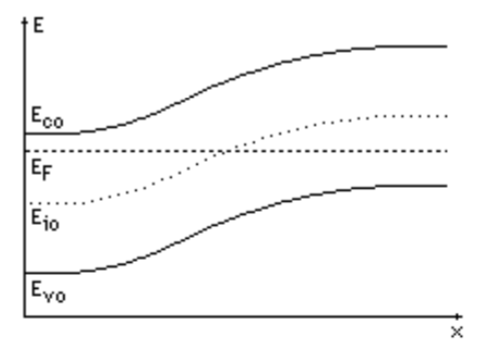
\includegraphics[width=0.6\textwidth]{Courbe.PNG}
    \caption{Courbure des bandes d'énergies à la jonction}
    \label{fig:Courbure}
\end{figure}
\subsubsection{Potentiel interne à l'équilibre}
On relie la densité de charge au potentiel au travers de l'équation de Poisson
\begin{equation}
\frac { d ^ { 2 } \Phi } { d x ^ { 2 } } = - \frac { q } { \varepsilon _ { s } } \left[ p ( x ) - n ( x ) + N _ { D } ^ { + } ( x ) - N _ { A } ^ { - } ( x ) \right]
\end{equation}
Il n'existe pas de solution analytique si on repart des expression des porteurs complettes, on fera donc certaines approximations :\\
\textbf{Quasi-neutralité :} Si une région du semiconducteur a une charge d'espace faible on peut l'approximer par une zone électriquement neutre
\begin{gather}
p ( \overline { r } ) - n ( \overline { r } ) + N _ { D } ( \overline { r } ) - N _ { A } ( \overline { r } ) = 0\\
p . n = n _ { i } ^ { 2 } \Leftrightarrow \quad \text{selon le dopage respectivement P ou N}\\ p ( \overline { r } ) = \frac { 1 } { 2 } \left[ N _ { A } ( \overline { r } ) + \sqrt { N _ { A } ^ { 2 } ( \overline { r } ) + 4 n _ { i } ^ { 2 } } \right]\quad\text{ou}\quad n ( \overline { r } ) = \frac { 1 } { 2 } \left[ N _ { D } ( \overline { r } ) + \sqrt { N _ { D } ^ { 2 } ( \overline { r } ) + 4 n _ { i } ^ { 2 } } \right] 
\end{gather}
On fera les approximations suivantes dans le cas P pour faciliter les calculs
\begin{gather}
p ( \overline { r } ) = N _ { A } ( \overline { r } ) \quad , \quad n ( \overline { r } ) = \frac { n _ { i } ^ { 2 } } { N _ { A } ( \overline { r } ) }\\
\Phi ( \overline { r } ) = \frac { E _ { i o } - E _ { F } } { q } - \frac { k T } { q } \ln \left[ \frac { N _ { A } ( \overline { r } ) } { n _ { i } } \right]\\
\operatorname { grad } \Phi ( \overline { r } ) = - \frac { k T } { q } \operatorname { grad } \left[ \ln N _ { A } ( \overline { r } ) \right]
\end{gather}
Et les approximations suivantes dans le cas N pour faciliter les calculs
\begin{gather}
n ( \overline { r } ) = N _ { D } ( \overline { r } ) \quad , \quad p ( \overline { r } ) = \frac { n _ { i } ^ { 2 } } { N _ { D } ( \overline { r } ) }\\
\Phi ( \overline { r } ) = \frac { E _ { i o } - E _ { F } } { q } + \frac { k T } { q } \ln \left[ \frac { N _ { D } ( \overline { r } ) } { n _ { i } } \right]\\
\operatorname { grad } \Phi ( \overline { r } ) = + \frac { k T } { q } \operatorname { grad } \left[ \ln N _ { D } ( \overline { r } ) \right]
\end{gather}
\textbf{Déplétion :} On suppose que dans la zone de jonction, les porteurs ont migrés et la zone est dépeuplé. Les Donneurs et accepteurs sont donc ionisés, on admet la relation 
\begin{equation}
| p ( x ) - n ( x ) | < < \left| N _ { D } ^ { + } ( x ) - N _ { A } ^ { - } ( x ) \right|
\end{equation}
On peut alors l'utiliser dans l'équation de Poisson
\begin{equation}
\frac { d ^ { 2 } \Phi( \overline { r } ) } { d ( \overline { r } ) ^ { 2 } } = - \frac { q } { \epsilon _ { s } } \left[ N _ { A } ( \overline { r } ) - N _ { D } ( \overline { r } ) \right]
\end{equation}
\subsubsection{Courant et coefficient de diffusion de porteurs}
À partir de la condition d'équilibre entre le potentiel de rappel et le courant de diffusion on ce s équations
\begin{equation}
\begin{array} { l } { J _ { n } = q \left( n _ { o } \mu _ { n } \mathcal {E } _ { o } + D _ { n } \frac { d n _ { o } } { d x } \right) = 0 } \\ { J _ { p } = q \left( p _ { o } \mu _ { p } \mathcal { E } _ { o } - D _ { p } \frac { d p _ { o } } { d x } \right) = 0 } \end{array}
\end{equation}
Nous devons d'abord calculer les valeurs des gradients. Nous connaisont les concentrations de porteurs donc 

\begin{equation}
\begin{array} { l } { n _ { o } ( x ) = n _ { i } e ^ { \left( E _ { F } - E _ { i o } \right) / k T } e ^ { q \Phi _ { o } ( x ) / k T } } \\ { p _ { o } ( x ) = n _ { i } e ^ { \left( E _ { i o } - E _ { F } \right) / k T } e ^ { - q \Phi _ { o } ( x ) / k T } } \end{array}
\end{equation}
et donc les gradients valent
\begin{equation}
\frac { d n _ { o } } { d x } = \frac { q } { k T } n _ { o } ( x ) \frac { d \Phi _ { o } } { d x } \quad,\quad \frac { d p _ { o } } { d x } = \frac { - q } { k T } p _ { o } ( x ) \frac { d \Phi _ { o } } { d x }\quad,\quad
\frac { d \Phi _ { o } } { d x } = - \mathcal { E }_0
\end{equation}
Les coefficients de diffusions sont maintenant faciles à calculer, la dérivé du potentiel est l'inverse du champ électrique
\begin{gather}
-n _ { o } \mu _ { n } \mathcal { E } _ { o } = D _ { n } \frac { d n _ { o } } { d x } \quad\Leftrightarrow\quad D _ { n } = \mu _ { n } \frac { k T } { q }\\
p _ { o } \mu _ { p } \mathcal { E } _ { o } = D _ { p } \frac { d p _ { o } } { d x }\quad\Leftrightarrow\quad D _ { p } = \mu _ { p } \frac { k T } { q }\\
\end{gather}
\subsubsection{Équations de transport d’un semiconducteur}
Dans le cas général de non-équilibre (tension appliquée)
\begin{equation}
\phi _ { 0 } ( x ) \rightarrow \phi ( x ) \quad  \mathcal { E } _ { 0 } ( x ) \rightarrow  \mathcal { E } ( x )\quad n _ { 0 } ( x ) \rightarrow n ( x ) \quad p _ { 0 } ( x ) \rightarrow p ( x )
\end{equation}
les courant sont
\begin{gather}
\begin{array} { l } { \overline { J } _ { n } = q \left( n \mu _ { n } \overline { \mathcal { E } } + D _ { n } \nabla n \right) } \\ { \overline { J } _ { p } = q \left( p \mu _ { p } \overline { \mathcal { E } } - D _ { p } \nabla p \right) } \end{array} \\
J = \vec { J } _ { n} + \overline { J } _ { P } + \varepsilon _ { s } \frac { \partial \overline { \mathcal{E} } } { \partial t }
\end{gather}
Le dernier terme est le courant de déplacement du à la variation du champ extérieur.\\
Nous avons besoin des équations de continuité des porteurs pour compléter l'équation précédente. Nous listons donc les phénomènes présents :
\begin{itemize}
    \item Les forces extérieurs appliquent une divergence de la densité de courant local $\nabla\cdot  \left( \overline { J } _ { n } \right) \text { ou } \nabla\cdot  \left( \overline { J } _ { p } \right)$
    \item La recombinaison par transfert d'un trou/électron dans la bande de conduction/valence respectivement $U _ { p } \left( U _ { n } \right)$
    \item La génération peut générer localement des trous/électrons par pair par illumination par exemple $G _ { n } \left( G _ { p } \right)$
\end{itemize}
Par conservation des porteurs on peut écrire la relation
\begin{equation}
\begin{aligned} \frac { \partial n } { \partial t } & = + \frac { 1 } { q } \nabla\cdot  \overline { J } _ { n } + G _ { n } - U _ { n } \\ \frac { \partial p } { \partial t } & = - \frac { 1 } { q } \nabla\cdot  \overline { J } _ { p } + G _ { p } - U _ { p } \end{aligned}
\end{equation}
Ces deux équations sont appelées équations de transport, elles décrivent l'évolution des porteurs et donne ainsi accès à la distribution et par conséquent aux champs.
\subsubsection{Quasi-niveaux de Fermi}
Soit les concentrations de porteurs à l'équilibre
\begin{equation}
\begin{array} { l } { n _ { o } ( \overline { r } ) = n _ { i } e ^ { \left( E _ { F } - E _ { i o } \right) / k T } e ^ { q \Phi _ { o } ( \overline { r } ) / k T } } \\ { p _ { o } ( \overline { r } ) = n _ { i } e ^ { \left( E _ { i o } - E _ { F } \right) / k T } e ^ { - q \Phi _ { o } ( \overline { r } ) / k T } } \\ { n _ { o } ( \overline { r } ) \cdot p _ { o } ( \overline { r } ) = n _ { i } ^ { 2 } ( T ) } \end{array}
\end{equation}
Le quasi niveau de Fermi est une adaptation de ces formules tel que en présence d'un potentiel externe on obtienne
\begin{equation}
\begin{array} { l } { n ( \overline { r } ; t ) = n _ { i } e ^ { \left[ E _ { F , n } ( \overline { r } , t ) - E _ { i o } \right] / k T } e ^ { q \Phi ( \overline { r } ; t ) / k T } } \\ { p ( \overline { r } ; t ) = n _ { i } e ^ { \left[ E _ { i o } - E _ { F , p } ( \overline { r } , t ) \right] / k T } e ^ { - q \Phi ( \overline { r } ; t ) / k T } } \\ { n ( \overline { r } ; t ) p ( \overline { r } ; t ) = n _ { i } ^ { 2 } ( T ) e ^ { \left[ E _ { F , n } ( \overline { r } , t ) - E _ { F , p } ( \overline { r } , t ) \right] / k T } } \end{array}
\end{equation}
Ainsi, on définit le niveau de Fermi constant comme variable dans l'espace, On définit donc les gradients de porteurs comme 
\begin{gather}
n = n \left( \nabla  E _ { F , n } + q \nabla  \Phi \right) / k T\\
p = - p \left( \nabla  E _ { F , p } + q \nabla  \Phi \right) / k T
\end{gather}
\section{Génération Recombinaison}
Les phénomènes de génération/recombinaison sont l'apparition/annulation d'un électron et d'un trou simultanément. Ces phénomènes respectent l'équilibre en tous temps.
\subsection{Génération de porteurs libres}
Un électron obtenant une énergie suffisante pour quitter la bande de valence et monter dans la bande de conduction est la génération. Il en existe plusieurs types :
\begin{itemize}
    \item Génération intrinsèque : l'électron obtient une énergie $E\geq E_g$ et monte dans la bande de conduction
    \item Génération électron extrinsèque : un centre donneur voit son électron recevoir une énergie suffisante pour monter dans la bande de conduction $E > E_c-E_R$, cela ne génère pas une paire mais un électron en excès
    \item Génération trous extrinsèque : un donneur ionisé peut obtenir un électron de la bande de valence si celui-ci obtient une énergie $E> E _ { r } - E _ { v }$, cela crée un trou en excès dans la bande de valence
    \item De manière analogue on peu définir tous des génération possibles
\end{itemize}
L'énergie permettant la migration d'un porteur peut être fournie par un photon, auquel cas son énergie est 
\begin{equation}
E = h v = h c / \lambda\quad,\quad \lambda ( \mu m ) < \frac { 1,24 } { E _ { g } ( e V ) } ( \mu m )
\end{equation}
L'énergie nécessaire moyenne dans le cas d'un semiconducteur est supérieur à $E_g$ car les deux porteurs ainsi crées ont une énergie cinétique après la collision.
\subsubsection{ Recombinaison de porteurs}
L'excès en porteur libres est réduit par le mécanisme de recombinaison. Il existe deux mécanismes de recombinaison :
\begin{itemize}
\item Recombinaison directe : un électron perd son énergie et rempli une place libre, annulant au passage un trou. Conserve ne crée pas d'excès de porteurs.
\item Capture par impuretés : une impureté ou un centre accepteur
/donneur ionisé peut capturer un électron dans la bande de conduction, celui-ci se trouve dans la bande extrinsèque. Crée un excès de trous. Une seconde transition vers la bande de valence peut compléter la recombinaison.
\end{itemize}
L'énergie ainsi émise peut se dégager souss trois formes différentes :
\begin{itemize}
    \item Recombinaison radiative : un photon d'énergie $hv$ est émis (diode émettrice).
    \item Recombinaison Auger : l'énergie émise peut être simplement captée par un électron qui montera lui même au seuil énergétique.
    \item Recombinaison Phonon : l'énergie est transféré au réseau cristallin sous la forme de phonons 
\end{itemize}
Il faut différencier la recombinaison en surface et à l'intérieur du matériau, cela est du à rupture de la périodicité. Soit la recombinaison interne et en surface
\begin{equation}
\begin{aligned} U _ { n } = \frac { n - n _ { o } } { \tau _ { n } } &\quad,\quad U _ { p } = \frac { p - p _ { o } } { \tau _ { p } } \\ S _ { n } = s _ { n } \left( n - n _ { o } \right) & \quad,\quad S _ { p } = s _ { p } \left( p - p _ { o } \right) \end{aligned}
\end{equation}

\subsubsection{Gradient de porteur}
En introduisant les phénomènes de génération/recombinaison et en résolvant les gradients on obtient à l'équilibre (pas de courant ni tension)
\begin{gather}
\frac { \partial n } { \partial t } = G - U = G - \frac { n - n _ { o } } { \tau }\\
\frac { \partial p } { \partial t } = G - U = G - \frac { p - p _ { o } } { \tau }
\end{gather}
On trouve l'excès de porteur initial
\begin{equation}
n = n _ { o } + \tau G \quad,\quad p = p _ { o } + \tau G
\end{equation}
Et en éliminant $G$ on trouve le retour à l'équilibre
\begin{equation}
\begin{array} { c } { n ( t ) = n _ { o } + \left[ n \left( t _ { o } \right) - n _ { o } \right] e ^ { - \left( t - t _ { o } \right) / \tau } = n _ { o } + \tau G e ^ { - \left( t - t _ { o } \right) / \tau } } \\ { p ( t ) = p _ { o } + \tau G e ^ { - \left( t - t _ { o } \right) / \tau } } \end{array}
\end{equation}
\begin{figure}[H]
    \centering
    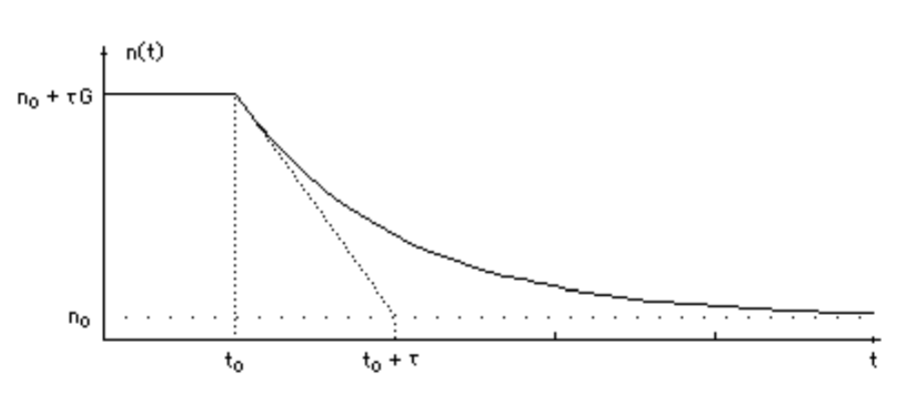
\includegraphics[width=0.6\textwidth]{gradUG.PNG}
    \caption{Gradient de porteur ne présence de génération et recombinaison}
    \label{fig:gradUG}
\end{figure}

\subsubsection{Équations de transport - Conditions aux limites}
On repart du cas ou tous les centres donneurs sont ionisés, les équation de Poisson, transport, diffusion et densité de courant sont
\begin{gather}
\nabla^2 \Phi = - \nabla\cdot \overline { \mathcal { E } } = - \frac { q } { \epsilon _ { s } } \left( p - n + N _ { D } - N _ { A } \right)\\
\frac { \partial n } { \partial t } = + \frac { 1 } { q } \nabla\cdot  \overline { J } _ { n } + G _ { n } - U _ { n }\\
\frac { \partial p } { \partial t } = - \frac { 1 } { q } \nabla\cdot  \overline { J } _ { p } + G _ { p } - U _ { p }\\
\overline { J } = \overline { J } _ { n } + \overline { J } _ { p } + \epsilon _ { s } \frac { \partial \overline { \mathcal { E } } } { \partial t }\\
\overline { J } _ { n } = q \left( n \mu _ { n } \overline { \mathcal { E } } + D _ { n } \nabla  n \right) \quad , \quad D _ { n } = \mu _ { n } \frac { k T } { q }\\
\overline { J } _ { p } = q \left( p \mu _ { p } \overline { \mathcal { E } } - D _ { p } \nabla  p \right) \quad , \quad D _ { p } = \mu _ { p } \frac { k T } { q }\\
\end{gather}
Il nous faut à présent les hypothèses sur le semiconducteur :
\begin{itemize}
    \item Les contacts par lesquels sont appliqués les potentiels sont ohmiques
    \item Les contacts ne présentent pas d'excès de porteurs
    \item L'interface sans contact est avec le vide, et suit les équations de continuité
    \begin{equation}
    \epsilon _ { s } \left( \nabla \Phi . \overline { n } _ { s c } \right) + \epsilon _ { i } \left( \nabla \Phi . \overline { n } _ { i } \right) = q N _ { s }
    \end{equation}
    donc la seule densité de courant en ces pointes est la recombinaison de surface de normal $\overline{n}$
    \begin{equation}
    \overline { J } _ { n } \cdot \overline { n } _ { s c } = - q S _ { n } \quad,\quad \overline { J } _ { p } \overline { n } _ { s c } = + q S _ { p }
    \end{equation}
\end{itemize}
Nous considérons maintenant le régime stationnaire, les équations de continuités sont 
\begin{equation}
\begin{array} { l } { D \frac { d ^ { 2 } n } { d x ^ { 2 } } + G - \frac { n - n _ { o } } { \tau } = 0 } \\ { D \frac { d ^ { 2 } p } { d x ^ { 2 } } + G - \frac { p - p _ { o } } { \tau } = 0 } \end{array}
\end{equation}
Dont les solutions génrales sont 
\begin{equation}
\begin{array} { l } { n ( x ) = n _ { o } + G \tau + A _ { n } e ^ { - x / L _ { D } } + B _ { n } e ^ { x / L _ { D } } } \\ { p ( x ) = p _ { o } + G \tau + A _ { p } e ^ { - x / L _ { D } } + B _ { p } e ^ { x / L _ { D } } } \end{array}
\end{equation}
avec $L _ { D } = \sqrt { D \tau }$. On introduit maintenant les conditions limites.\\
Les densités de porteurs doivent être finis en tous points, et il existe une valeur d'équilibre :
\begin{equation}
B _ { n } = B _ { p } = 0\quad,\quad n ( \infty ) = n _ { o } + G \tau \quad,\quad p ( \infty ) = p _ { o } + G \tau
\end{equation}
La recombinaison en surface impose 
\begin{gather}
D \left( \frac { d n } { d x } \right) _ { x = 0 } = s \left[ n ( 0 ) - n _ { o } \right]\\
D \left( \frac { d p } { d x } \right) _ { x = 0 } = s \left[ p ( 0 ) - p _ { o } \right]
\end{gather}
On trouve finalement la solution recherchée, avec $R = s T / L _ { D }$
\begin{equation}
\begin{array} { l } { n ( x ) = n _ { o } + G \tau \left( 1 - \frac { R } { 1 + R } e ^ { - x / L _ { D } } \right) } \\ { p ( x ) = p _ { o } + G \tau \left( 1 - \frac { R } { 1 + R } e ^ { - x / L _ { D } } \right) } \end{array}
\end{equation}
L'interprétation de ces résultats est que la recombinaison suplémentaire à la surface est la source d'un gradient de diffusion vers celles-ci.\\
Il existe le cas particulier $s \rightarrow \infty$ qui correspond au cas d'un contact ohmique, la recombinaison y est infinie et l'excès de porteur s'y annule.\\
En pratique la neutralité n'est pas respecté en surface, il existe donc un champ et des gradients et distributions etc.
\subsubsection{Recombinaison indirecte}
Pour calculer les taux de recombinaisons, nous devons partir des interprétations physique. Soit les centres de recombinaisons accepteurs d'énergie $E_r$, la concentration d'électrons $n_r \leq N_r$ occupant ces centres. Nous travaillons ici avec des recombinaisons et générations spontanées, celles-ci peuvent donc être l'oeuvre d'agitation thermique. \\
Soit $U_{n,a}$ le taux de recombinaison par capture d'un électron dans un centre neutre. Celui-ci est proportionnel à la concentration d'électrons et la concentration en en centres vides.
\begin{equation}
U _ { n , a } = c _ { n } n \left( N _ { r } - n _ { r } \right)
\end{equation}
avec $c_n$ la probabilité de capture.\\
Soit $U_{n,b}$, la génération thermique d'un électron depuis un centre négatif. Celui-ci est proportionnel aux centres occupés et au nombre de places libres dans la bande de conduction.
\begin{equation}
U _ { n , b } = e _ { n } n _ { r } p _ { c }
\end{equation}
avec $e_n$ la probabilité d'émission vers la bande de conduction. Ne connaissant pas $p_c$ on écrira l'expression comme ceci
\begin{equation}
U _ { n , b } = c _ { n } n _ { r } n _ { 1 }
\end{equation}
Les taux nets respectivement pour les électrons et trous sont donc
\begin{gather}
U _ { n } = c _ { n } \left[ n \left( N _ { r } - n _ { r } \right) - n _ { r } n _ { 1 } \right]\\
U _ { p } = c _ { p } \left[ p n _ { r } - \left( N _ { r } - n _ { r } \right) p _ { 1 } \right]
\end{gather}
Dans le cas d'un semiconducteur sans génération, la neutralité est respecté et $U_n=U_p=0$ et donc
\begin{gather}
n _ { o } ( \overline { r } ) = n _ { i } e ^ { \left( E _ { F } - E _ { i o } \right) / k T } e ^ { q \Phi _ { o } ( \overline { r } ) / k T }\quad,\quad p _ { o } ( \overline { r } ) = n _ { i } e ^ { \left( E _ { i o } - E _ { F } \right) / k T } e ^ { - q \Phi _ { o } ( \overline { r } ) / k T }\\
n _ { r o } ( \overline { r } ) = \frac { N _ { r } } { 1 + e ^ { \left( E _ { r o } - E _ { F } \right) / k T } e ^ { - q \Phi _ { o } ( \overline { r } ) / k T } }\\
n _ { 1 } = n _ { i } e ^ { \left( E _ { r o } - E _ { i o } \right) / k T } \quad,\quad p _ { 1 } = n _ { i } e ^ { - \left( E _ { r o } - E _ { i o } \right) / k T } \quad,\quad n _ { 1 } p _ { 1 } = n _ { i } ^ { 2 }
\end{gather}
Les valeurs $n_1$ et $p_1$ s'avèrent être les valeurs d'équilibre et sont valables aussi hors équilibre.\\
Pour finir nous développons l'équation de continuité sur les électrons capturés dans les centres, celle-ci est influencé par la génération et la recombinaison venant des deux bandes adjacentes
\begin{gather}
\frac { \partial n _ { r } } { \partial t } = U _ { n } - U _ { p } + G _ { p } - G _ { n }\\
\nabla^2 \Phi = - \nabla\cdot \overline { \mathcal { E} } = - \frac { q } { \epsilon _ { s } } \left( p - n - n _ { r } + N _ { D } - N _ { A } \right)
\end{gather}
Le terme $n_r$ est in fine négligeable dans l'équation de neutralité de la charge.
\subsubsection{Modèle de Shockley-Read-Hall en régime permanent}
En régime permanent nous admettons la situation d'équilibre
\begin{gather}
\frac { \partial n } { \partial t } = \frac { \partial p } { \partial t } = \frac { \partial n _ { r } } { \partial t } = 0\\
G = G _ { n } = G _ { p }\quad,\quad U _ { n } = U _ { p }
\end{gather}
À partir de l'égalité des génération des deux cotés de la bande nous pouvons écrire
\begin{equation}
n _ { r } = \frac { N _ { r } \left( c _ { n } n + c _ { p } p _ { 1 } \right) } { c _ { n } \left( n + n _ { 1 } \right) + c _ { p } \left( p + p _ { 1 } \right) }
\end{equation}
En injectant 
\begin{gather}
U _ { n } = c _ { n } \left[ n \left( N _ { r } - n _ { r } \right) - n _ { r } n _ { 1 } \right]\\
U _ { p } = c _ { p } \left[ p n _ { r } - \left( N _ { r } - n _ { r } \right) p _ { 1 } \right]
\end{gather}
on trouve
\begin{gather}
\begin{array} { l } { U _ { n } = U _ { p } = \frac { c _ { n } c _ { p } N _ { r } \left( p n - n _ { i } ^ { 2 } \right) } { c _ { n } \left( n + n _ { 1 } \right) + c _ { p } \left( p + p _ { 1 } \right) } } \\ { U _ { n } = U _ { p } = \frac { p n - n _ { i } ^ { 2 } } { \tau _ { p o } \left( n + n _ { 1 } \right) + \tau _ { n o } \left( p + p _ { 1 } \right) } } \end{array}\\
\tau _ { n o } = \frac { 1 } { N _ { r } c _ { n } } \quad,\quad \tau _ { p o } = \frac { 1 } { N _ { r } c _ { p } }
\end{gather}
Le numérateur est forcément nulle et donc les taux également. Nous pouvons en déduire les durées de vie des porteur en régime permanent
\begin{equation}
\begin{aligned} \boldsymbol { \tau } _ { n } & = \frac { n - n _ { o } } { p n - n _ { i } ^ { 2 } } \left[ \tau _ { p o } \left( n + n _ { 1 } \right) + \tau _ { n o } \left( p + p _ { 1 } \right) \right] \\ \tau _ { p } & = \frac { p - p _ { o } } { p n - n _ { i } ^ { 2 } } \left[ \tau _ { p o } \left( n + n _ { 1 } \right) + \tau _ { n o } \left( p + p _ { 1 } \right) \right] \end{aligned}
\end{equation}
L'équilibre n'est pas forcément toujours atteint, imaginons donc le cas de faible injection avec quelques résidus dont les valeurs sont égales supposément $\delta n = \delta p$
\begin{gather}
p n - n _ { i } ^ { 2 } \approx p _ { o } \delta n + n _ { o } \delta p\\
U _ { n } = U _ { p } = \frac { p _ { o } \delta n + n _ { o } \delta p } { \tau _ { p o } \left( n _ { o } + n _ { 1 } \right) + \tau _ { n o } \left( p _ { o } + p _ { 1 } \right) } =\frac { \delta n \left( p _ { o } + n _ { o } \right) } { \tau _ { p o } \left( n _ { o } + n _ { 1 } \right) + \tau _ { n o } \left( p _ { o } + p _ { 1 } \right) }
\end{gather}
Soit finalement les temps de vies
\begin{equation}
\tau = \tau _ { n } = \tau _ { p } = \frac { \tau _ { p o } \left( n _ { o } + n _ { 1 } \right) + \tau _ { n o } \left( p _ { o } + p _ { 1 } \right) } { p _ { o } + n _ { o } }
\end{equation}
Dans l'hypothèse de faible injection on suppose également que la concentration d'électrons capturés par des impuretés est constants $ { n } _ { r } \approx  { n } _ { r o }$, et que celle-ci est négligeable par rapport à la concentration de porteurs libres. On peut donc de ce cas uniquement travailler avec les équations de transport.\\
On remarque que le de temps vie des porteurs est donc fonction du niveau de Fermi. Plus celui-ci est proche de $E_i$ plus le temps de vie des porteurs est grand.\\
\begin{figure}[H]
    \centering
    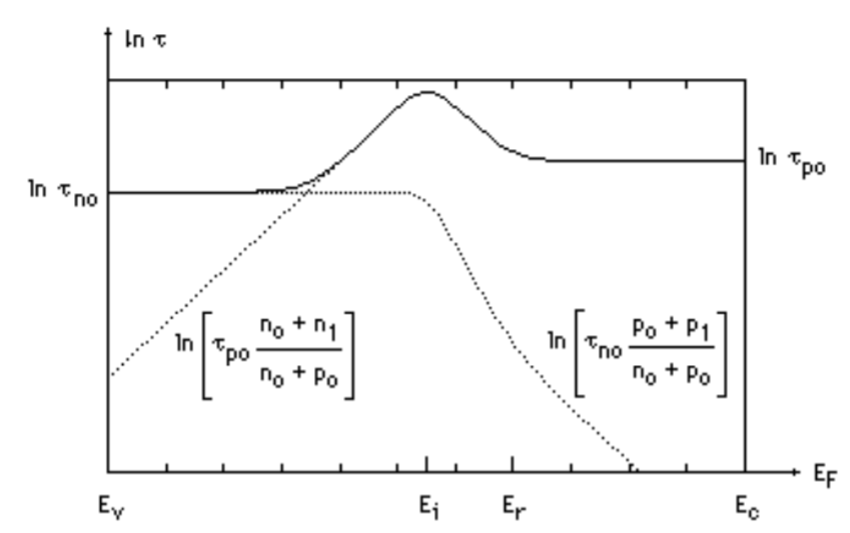
\includegraphics[width=0.6\textwidth]{tau.PNG}
    \caption{Temps de vie des porteurs en fonction du niveau de Fermi sous l'hypothèse de faible injection}
    \label{fig:tau}
\end{figure}
Sur la figure on distingue deux plages de valeur remarquables. Pour un semiconducteur de type P on a les approximations suivante qui réduisent l'expression à
\begin{gather}
p _ { o } \gg p _ { 1 } \gg n _ { o } \text { et } p _ { o } \gg n _ { 1 }\\
U _ { n } = U _ { p } = \frac { n - n _ { o } } { \tau _ { n o } } \quad,\quad \tau _ { n } = \tau _ { p } = \tau _ { n o } = \frac { 1 } { N _ { r } c _ { n } }
\end{gather}
La mobilité est donc inversement proportionnelle au nombre de centre recombinants et à la valeur $c_n$ la probabilité de capture d'un électron. Cela parait évident que ce soit le temps de vie des minoritaires qui soit utilisé car dès que l'un d'entre eux est capturé par un centre recombinant il peut aisément continuer jusqu'à la bande suivante. \\
Par un raisonnement analogue, on trouve le temps de vie pour un semiconducteur de type N
\begin{gather}
n _ { o } \gg n _ { 1 } \gg p _ { o } \text { et } n _ { o } \gg p _ { 1 }\\
U _ { n } = U _ { p } = \frac { p - p _ { o } } { \tau _ { p o } } , \tau _ { n } = \tau _ { p } = \tau _ { p o } = \frac { 1 } { N _ { r } c _ { p } }
\end{gather}
\begin{figure}[H]
    \centering
    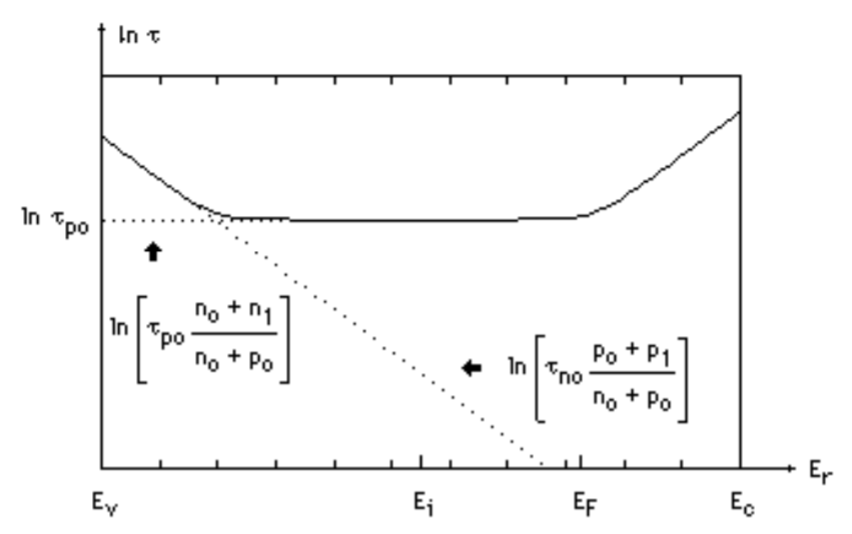
\includegraphics[width=0.6\textwidth]{tauR.PNG}
    \caption{Temps de vie des porteurs en fonction du niveau intrinsèque dans un conducteur de type N}
    \label{fig:tauR}
\end{figure}

\subsubsection{Modèle de la recombinaison en surface}
Soit es centre recombinant de la surface, ceux-ci sont différents des centre dans le semiconducteur. Ils sont présent en nombre $N_s$ et localiser à un niveau extrinsèque $E_s$. On utilise le modèle de Schockley-Read-Hall de la recombinaison indirecte. Par un raisonnement analoque à celui de la section précédente on obtient la recombinaison en nombre par surface avec les concentrations 
\begin{gather}
S _ { n } = S _ { p } = \frac { c _ { n } c _ { p } N _ { s } \left( p _ { s } n _ { s } - n _ { i } ^ { 2 } \right) } { c _ { n } \left( n _ { s } + n _ { 1 s } \right) + c _ { p } \left( p _ { s } + p _ { 1 s } \right) }\\
n _ { 1 s } = n _ { i } e ^ { \left( E _ { s } - E _ { i , s } \right) / k T } \quad,\quad p _ { 1 s } = n _ { i } e ^ { - \left( E _ { s } - E _ { i , s } \right) / k T } \quad,\quad p _ { 1 s } n _ { 1 s } = n _ { i } ^ { 2 }
\end{gather}
grâce aux définitions $S _ { n } = s _ { n } \left( n - n _ { o } \right) \quad , \quad S _ { p } = s _ { p } \left( p - p _ { o } \right)$ on trouve l'expression en vitesse de recombinaison
\begin{gather}
\begin{aligned} s _ { n } & = \frac { c _ { n } c _ { p } N _ { s } \left( p _ { s } n _ { s } - n _ { i } ^ { 2 } \right) } { \left[ c _ { n } \left( n _ { s } + n _ { 1 s } \right) + c _ { p } \left( p _ { s } + p _ { 1 s } \right) \right] \left( n _ { s } - n _ { s o } \right) } \\ s _ { p } & = \frac { c _ { n } c _ { p } N _ { s } \left( p _ { s } n _ { s } - n _ { i } ^ { 2 } \right) } { \left[ c _ { n } \left( n _ { s } + n _ { 1 s } \right) + c _ { p } \left( p _ { s } + p _ { 1 s } \right) \right] \left( p _ { s } - p _ { s o } \right) } \end{aligned}
\end{gather}
Idem, dans le cas de faible excès de porteur par rapport à l'équilibre
\begin{gather}
\begin{aligned} \delta n _ { s } & = n _ { s } - n _ { s o } \ll n _ { s o } \quad\text{ou}\quad p _ { s o } \\ \delta p _ { s } & = p _ { s } - p _ { s o } \ll n _ { s o } \quad\text{ou}\quad p _ { s o } \end{aligned}\\
\delta n _ { s } = \delta p _ { s }\\
\begin{aligned} S _ { n } & = S _ { p } = \frac { \delta n _ { s } c _ { n } c _ { p } N _ { s } \left( p _ { s o } + n _ { s o } \right) } { c _ { n } \left( n _ { s o } + n _ { 1 s } \right) + c _ { p } \left( p _ { s o } + p _ { 1 s } \right) } \\ s _ { n } = s _ { p } & = \frac { c _ { n } c _ { p } N _ { s } \left( p _ { s o } + n _ { s o } \right) } { c _ { n } \left( n _ { s o } + n _ { 1 s } \right) + c _ { p } \left( p _ { s o } + p _ { 1 s } \right) } \end{aligned}
\end{gather}
de nouveau on distingue les approximations des semiconducteurs respectivement de type P et N permettenant de simplifier l'expression précédente respectivement en
\begin{gather}
p _ { o } \gg p _ { 1 } \gg n _ { o } \text { et } p _ { o } \gg n _ { 1 } \quad,\quad n _ { o } \gg n _ { 1 } \gg p _ { o } \text { et } n _ { o } \gg p _ { 1 } \\
S _ { n } = S _ { p } = \left( n _ { s } - n _ { s o } \right) c _ { n } N _ { s } \quad , \quad s _ { n } = s _ { p } = c _ { n } N _ { s }\quad,\quad S _ { n } = S _ { p } = \left( p _ { s } - p _ { s o } \right) c _ { p } N _ { s } , s _ { n } = s _ { p } = c _ { p } N _ { s }
\end{gather}
Idem ici, le processus de capture des minoritaires détermine le taux de recombinaison.
\subsubsection{Recombinaison directe radiative}
La recombinaison radiative émet un photon en guise d'énergie perdu par l'électron. Le taux de recombinaison est, avec $U_b$ la génération thermique,
\begin{equation}
U = c p n - U _ { b }
\end{equation}
À l'équilibre thermodynamique, la génération totale est nulle
\begin{equation}
U = 0\quad,\quad U _ { b } = c n _ { i } ^ { 2 }\quad,\quad U = c \left( p n - n _ { i } ^ { 2 } \right)
\end{equation}
et par la relation de diffusion on trouve
\begin{equation}
\tau _ { n } = \frac { n - n _ { o } } { c \left( p n - n _ { i } ^ { 2 } \right) } , \quad \tau _ { p } = \frac { p - p _ { o } } { c \left( p n - n _ { i } ^ { 2 } \right) }
\end{equation}
Soit le cas habituel de faible excès de porteur 
\begin{gather}
\begin{array} { l l } { \delta n _ { s } = n _ { s } - n _ { s o } \ll n _ { s o } } & { \text { ou } p _ { s o } } \\ { \delta p _ { s } = p _ { s } - p _ { s o } \ll n _ { s o } } & { \text { ou } p _ { s o } } \end{array}\\
\delta n = \delta p\\
p n - n _ { i } ^ { 2 } = \delta n \left( p _ { o } + n _ { o } \right)
\end{gather}
On peut donc simplifier les expressions
\begin{equation}
U = c \delta n \left( p _ { o } + n _ { o } \right) \quad , \quad \tau _ { n } = \tau _ { p } = \frac { 1 } { c \left( p _ { o } + n _ { o } \right) }
\end{equation}
Après simplification pour les dopages on obtient
\begin{equation}
\begin{array} { l } { \tau _ { n } = \tau _ { p } = \frac { 1 } { c p _ { o } } \quad,\quad \text { type } P } \\ { \tau _ { n } = \tau _ { p } = \frac { 1 } { c n _ { o } } \quad,\quad\text{ type } N } \end{array}
\end{equation}
On remarque que la recombinaison radiative est inversement proportionnelle aux porteurs majoritaires d'équilibre, elle nécessite donc des dopages très élevés pour diminuer au maximum la durée de vie.
\begin{figure}[H]
    \centering
    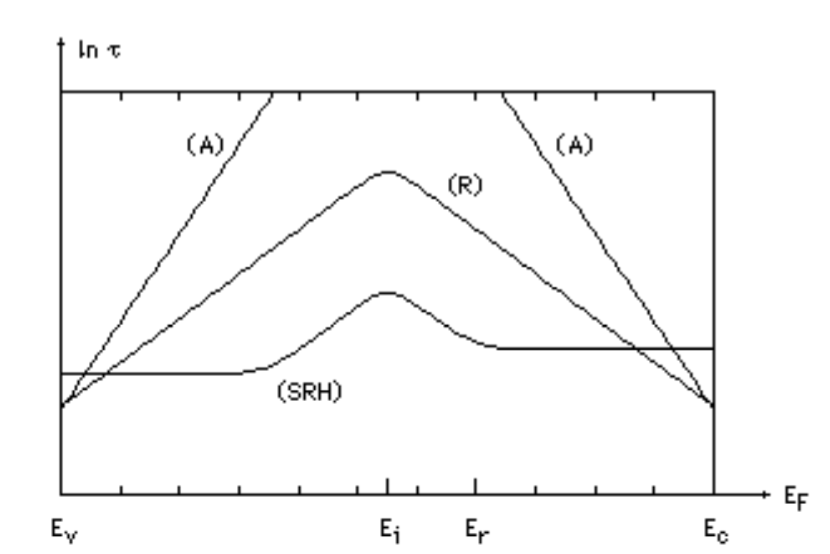
\includegraphics[width=0.6\textwidth]{Recombinaison.PNG}
    \caption{Comparaison des temps de vies (R)adiative, (A)uger, et (SRH) Shockley-Read-Hall}
    \label{fig:recombinaison}
\end{figure}
\subsubsection{Recombinaison Auger}
Ce méchanisme de recombinaison laisse un électron déscendre dans la bande de valence et donner toutes son énergie à un autre électrons dans n'importe quelle bande. Son taux de recombinaison est 
\begin{equation}
U = c _ { 1 } n ^ { 2 } p + c _ { 2 } p ^ { 2 } n - U _ { b }
\end{equation}
Même raisonnement 
\begin{equation}
U = 0 \quad,\quad U _ { b } = \left( c _ { 1 } n _ { o } + c _ { 2 } p _ { o } \right) n _ { i } ^ { 2 } \quad,\quad U = c _ { 1 } \left( n ^ { 2 } p - n _ { i } ^ { 2 } n _ { o } \right) + c _ { 2 } \left( p ^ { 2 } n - n _ { i } ^ { 2 } p _ { o } \right)
\end{equation}
Et on obtient les temsp de vie suivants
\begin{equation}
\begin{array} { l } { \tau _ { n } = \frac { n - n _ { o } } { c _ { 1 } \left( n ^ { 2 } p - n _ { i } ^ { 2 } n _ { o } \right) + c _ { 2 } \left( p ^ { 2 } n - n _ { i } ^ { 2 } p _ { o } \right) } } \\ { \tau _ { p } = \frac { p - p _ { o } } { c _ { 1 } \left( n ^ { 2 } p - n _ { i } ^ { 2 } n _ { o } \right) + c _ { 2 } \left( p ^ { 2 } n - n _ { i } ^ { 2 } p _ { o } \right) } } \end{array}
\end{equation}
Soit en faible excès
\begin{gather}
\begin{array} { l } { \delta n = n - n _ { o } \ll n _ { o } \quad\text{ou}\quad p _ { o } } \\ { \delta p = p - p _ { o } \ll n _ { o } \quad\text{ou}\quad p _ { o } } \end{array}
\end{gather}
Et donc par la fonction en régime permanent
\begin{gather}
\delta n = \delta p\\
n ^ { 2 } p - n _ { i } ^ { 2 } n _ { o } \approx \delta n \left( n _ { o } ^ { 2 } + 2 n _ { i } ^ { 2 } \right)
U = \delta n \left[ c _ { 1 } \left( n _ { o } ^ { 2 } + 2 n _ { i } ^ { 2 } \right) + c _ { 2 } \left( p _ { o } ^ { 2 } + 2 n _ { i } ^ { 2 } \right) \right]\\
\tau _ { n } = \tau _ { p } = \frac { 1 } { c _ { 1 } \left( n _ { o } ^ { 2 } + 2 n _ { i } ^ { 2 } \right) + c _ { 2 } \left( p _ { o } ^ { 2 } + 2 n _ { i } ^ { 2 } \right) }
\end{gather}
Et dans le cas de dopage 
\begin{gather}
\begin{array} { l } { \tau _ { n } = \tau _ { p } = \frac { 1 } { c _ { 2 } p _ { o } ^ { 2 } } \quad,\quad \text{type } P } \\ { \tau _ { n } = \tau _ { p } = \frac { 1 } { c _ { 1 } n _ { o } ^ { 2 } } \quad,\quad \text{type } N } \end{array}
\end{gather}
La recombinaison Auger est inversement quadratiquement proportionnelle au dopage et donc très présente dans les dispositifs de puissance.
\subsubsection{Combinaison des mécanismes de recombinaison}
Tout d'abord il est important de noter que des mécanismes de supplémentaires existe et n'ont pas été travaillé ici, pour en citer quelques uns les pièges, des centres multivalents, des successions de centres monovalents ou multivalents.\\
L'ensemble des mécanismes sont somme direct, la recombinaison est donc
\begin{equation}
U _ { n } = \sum _ { i } U _ { n , i } \quad,\quad U _ { p } = \sum _ { i } U _ { p , i }
\end{equation}
et les durées de vies par la continuité
\begin{equation}
\tau _ { n } = \frac { \delta n } { \sum _ { i } U _ { n , i } } , \quad \tau _ { p } = \frac { \delta p } { \sum _ { i } U _ { p , i } }
\end{equation}
Pour avoir des semiconducteurs rapides, c'est-à-dire avec des basses durées de vie de porteurs, on ajoute des impuretés qui ne sont pas des dopants dans le dispositif.
\subsubsection{Maintient de la neutralité électrique}
L'hypothèse de neutralité électrique est une simplification valable et pratique. Néanmoins elle n'est pas vrai dans tous les cas.\\
Soit un semiconducteur à l'équilibre en $t=0$. Une génération en $t>0$ provoque une rupture de la neutralité, ce qui donne naissance à un champ électrique.
\begin{gather}
\rho ( x ; t < 0 ) = q \left( p _ { o } - n _ { o } + N _ { D } \right) = 0\\
\rho ( x ; t \geq 0 ) = q \left( p - n + N _ { D } \right) \neq 0\\
\frac { \partial \mathcal { E } } { \partial x } = \frac { \rho ( x ; t \geq 0 ) } { \epsilon _ { s } }
\end{gather}
Nous négligeons la génération recombinaison. Le courant issu du champ est
\begin{gather}
J _ { n } = q n \mu _ { n } \mathcal { E } \quad,\quad J _ { p } = q p \mu _ { p } \mathcal { E }
\end{gather}
Dans le cas d'un dispositif de type N
\begin{gather}
p - p _ { o } \ll n _ { o } \quad,\quad\text{donc} \quad \quad p \ll n _ { o }\\
J _ { n } = q n _ { o } \mu _ { n } \mathcal { E } \quad,\quad J _ { p } = q p \mu _ { p } \mathcal { E } \quad,\quad  J = J _ { n } + J _ { p } \approx J _ { n }
\end{gather}
On injecte dans la continuité
\begin{gather}
\frac { \partial n } { \partial t } = \frac { 1 } { q } \frac { \partial J _ { n } } { \partial x } \quad,\quad  \frac { \partial p } { \partial t } = - \frac { 1 } { q } \frac { \partial J _ { p } } { \partial x }\\
- \frac { \partial ( p - n ) } { \partial t } = \frac { 1 } { q } \frac { \partial \left( J _ { n } + J _ { p } \right) } { \partial x } \approx \frac { 1 } { q } \frac { \partial J _ { n } } { \partial x } = \mu _ { n } n _ { o } \frac { \partial \mathcal { E } } { \partial x }\\
- \frac { \partial \rho ( x ; t ) } { \partial t } = \frac { q \mu _ { n } n _ { o } } { \epsilon _ { s } } \rho ( x ; t ) = \frac { \sigma _ { n } } { \epsilon _ { s } } \rho ( x ; t )
\end{gather}
Finalement en intégrant on obtient la charge d'espace en fonction du temps
\begin{equation}
\rho ( x ; t ) = \rho ( x ; 0 ) e ^ { - \sigma _ { n } t / \epsilon _ { s } }
\end{equation}
On appele le facteur exponentiel $\epsilon _ { s } / \sigma _ { n }$ le temps de relaxation diélectrique. Donc tant que le temps analysé est suppérieur d'un ordre de grandeur au temps de relaxation diélectrique, on peut assumer la neutralité électrique.
\subsection{Régime permanent}
Grâce à tous les résultats précédents nous pouvons écrire l'équation de continuité avec tous ses termes, génération, recombinaison, différence de concentration de porteur, gradient de porteurs
\begin{equation}
\frac { \partial p } { \partial t } = G - \frac { p - p _ { o } } { \tau _ { p o } } - \mu _ { p } \mathcal { E } \frac { \partial p } { \partial x } + D _ { p } \frac { \partial ^ { 2 } p } { \partial x ^ { 2 } }
\end{equation}
En utilisant cette équation dans les cas suivant nous pouvons résoudre tous les cas en régime permanent
\subsubsection{Génération continue}
soit un solide avec de la génération continue en $x=0$
\begin{equation}
D _ { p } \frac { \partial ^ { 2 } p } { \partial x ^ { 2 } } - \frac { p - p _ { o } } { \tau _ { p o } } = 0
\end{equation}
Le profile de porteur est de la forme suivante
\begin{figure}[H]
    \centering
    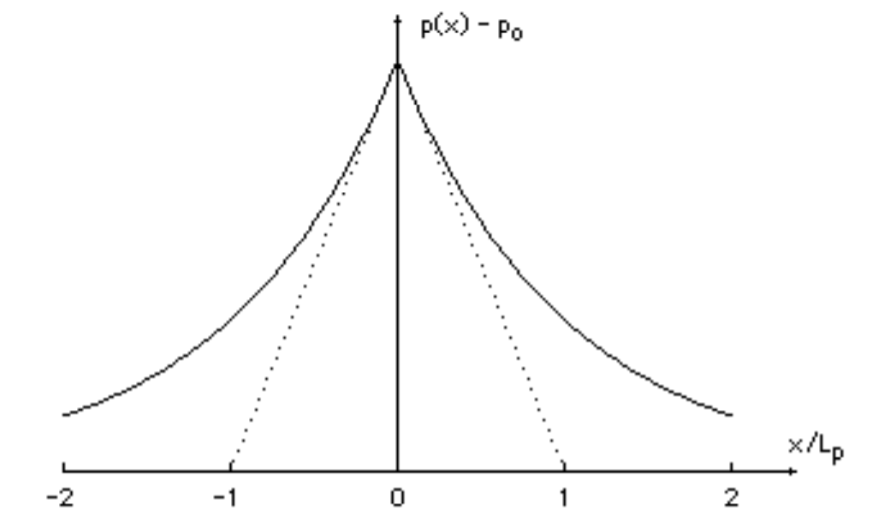
\includegraphics[width=0.6\textwidth]{porteur1.PNG}
    \caption{Distribution de porteurs à génération constante}
    \label{fig:port1}
\end{figure}
La solution de l'équation nécessite les conditions limites de retour à l'équilibre et de valeur initiale, avec $\delta p ( 0 )$ l'excès initial du à la génération et $L _ { p } = \sqrt { D _ { p } \tau _ { p o } }$ la longueur de diffusion
\begin{gather}
p \rightarrow p _ { o } \text { pour } | x | \rightarrow \infty\\
p ( x ) = p _ { o } + \delta p ( 0 ) e ^ { - x / L _ { p } } \text { pour } x > 0\\
p ( x ) = p _ { o } + \delta p ( 0 ) e ^ { + x / L _ { p } } \text { pour } x < 0
\end{gather}
Les trous générés diffusent et se recombinent selon une loi exponentielle jusqu'au retour à l'équilibre asymptotique. La distribution des trous est similaire à une constante près, en effet
\begin{equation}
n ( x ) = n _ { o } + p ( x ) - p _ { o }
\end{equation}
\subsubsection{Régime permanent avec génération et champ électrique}
L'équation ambipolaire devient alors
\begin{equation}
D _ { p } \frac { \partial ^ { 2 } p } { \partial x ^ { 2 } } - \mu _ { p } \mathcal { E } \frac { \partial p } { \partial x } - \frac { p - p _ { o } } { \tau _ { p o } } = 0
\end{equation}
et sa solution est 
\begin{gather}
p \rightarrow p _ { o } \text { pour } | x | \rightarrow \infty\\
\begin{array} { c } { p ( x ) = p _ { o } + \delta p ( 0 ) e ^ { - x / L _ { - } } \text { pour } x > 0 } \\ { p ( x ) = p _ { o } + \delta p ( 0 ) e ^ { + x / L _ { + } } }  { \text { pour } x < 0 } \end{array}
\end{gather}
Le longueurs de diffusion sont ici 
\begin{gather}
\begin{aligned} \frac { 1 } { L _ { - } } & = \sqrt { \left( \frac { \mu _ { p } \mathcal { E } } { 2 D _ { p } } \right) ^ { 2 } + \frac { 1 } { L _ { p } ^ { 2 } } } - \frac { \mu _ { p } \mathcal { E } } { 2 D _ { p } } \\ \frac { 1 } { L _ { + } } & = \sqrt { \left( \frac { \mu _ { p } \mathcal { E } } { 2 D _ { p } } \right) ^ { 2 } + \frac { 1 } { L _ { p } ^ { 2 } } } + \frac { \mu _ { p } \mathcal { E } } { 2 D _ { p } } \end{aligned}
\end{gather}
La présence de champ électrique détruit la symétrie de la distribution
\begin{figure}[H]
    \centering
    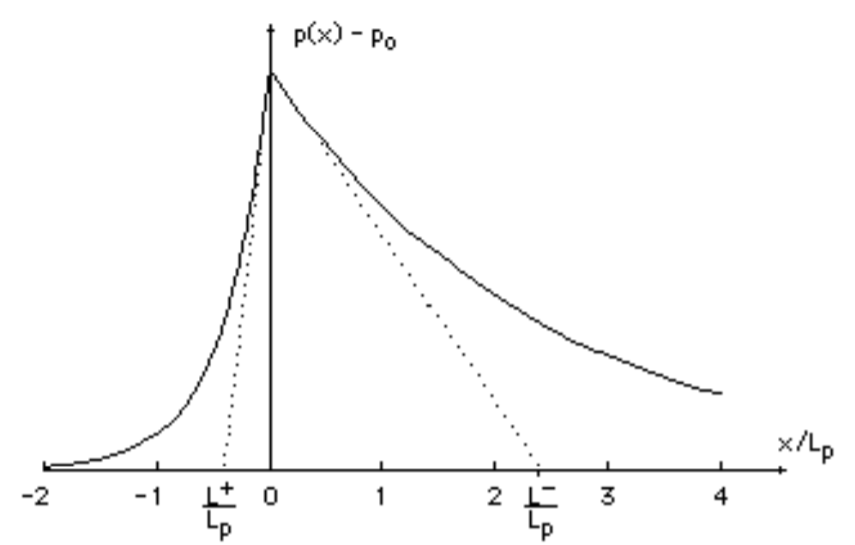
\includegraphics[width=0.6\textwidth]{porteur2.PNG}
    \caption{Distribution de porteurs à génération constante avec champ électrique}
    \label{fig:port2}
\end{figure}
Le champ s'oppose à la diffusion des porteurs. La distribution des trous est similaire à une constante près, en effet
\begin{equation}
n ( x ) = n _ { o } + p ( x ) - p _ { o }
\end{equation}
Deux approximation simplificatrices sont possibles ici, soit le champ est faible
\begin{gather}
| \mathcal { E } | \ll 2 k T / \left( q L _ { p } \right) \Leftrightarrow L _ { - } = L _ { + } = L _ { p }
\end{gather}
soit le champ est intense
\begin{gather}
| \mathcal { E } | \gg 2 k T / \left( q L _ { p } \right)\\
\frac { 1 } { L _ { - } } = \frac { D _ { p } } { \mu _ { p } \mathcal { E } L _ { p } ^ { 2 } } = \frac { 1 } { \mu _ { p } \mathcal { E } \tau _ { p o } }\quad,\quad\frac { 1 } { L _ { + } } = \frac { \mu _ { p } \mathcal { E } } { D _ { p } }
\end{gather}
\subsubsection{Génération pendant un intervalle de temps sous un champ}
Soit une génération abrupte delta-dirac
\begin{gather}
\begin{aligned} \delta p ( 0 ; 0 ) & = \delta p _ { o } \delta ( x ) \delta ( t ) \\ \delta n ( 0 ; 0 ) & = \delta p ( 0 ; 0 ) \end{aligned}
\end{gather}
La neutralité en tous points impose la neutralité locale donc
\begin{equation}
p ( x ; t ) - p _ { o } = n ( x ; t ) - n _ { o }
\end{equation}
L'équation ambipolaire est valable pour les trous et les électrons
\begin{equation}
\frac { \partial p } { \partial t } = \frac { \partial n } { \partial t } = - \frac { p - p _ { o } } { \tau _ { p o } } - \mu _ { p } \mathcal { I } \frac { \partial p } { \partial x } + D _ { p } \frac { \partial ^ { 2 } p } { \partial x ^ { 2 } }
\end{equation}
Comme précédemment avec les conditions limites on résout
\begin{gather}
p \rightarrow p _ { o } \text { pour } | x | \rightarrow \infty\\
p ( x ; t ) = p _ { o } + \frac { \delta p _ { o } } { 2 \sqrt { \pi D _ { p } t } } e ^ { - t / \tau _ { p } } e ^ { - \left( x - \mathcal { E } \mu _ { p } t \right) ^ { 2 } / 4 D _ { p } t }
\end{gather}
On peut dégager de l'équation de densité de porteurs un maximum dépendant du temps et son amplitude en fonction du temps
\begin{gather}
x = \mathcal { E } \mu _ { p } t \quad,\quad p \left( \mathcal { E } \mu _ { p } t ; t \right) = p _ { o } + \frac { \delta p _ { o } } { 2 \sqrt { \pi D _ { p } t } } e ^ { - t / \tau _ { p } }
\end{gather}
On peut voir ci-dessous comment le maximum se déplace 
\begin{figure}[H]
    \centering
    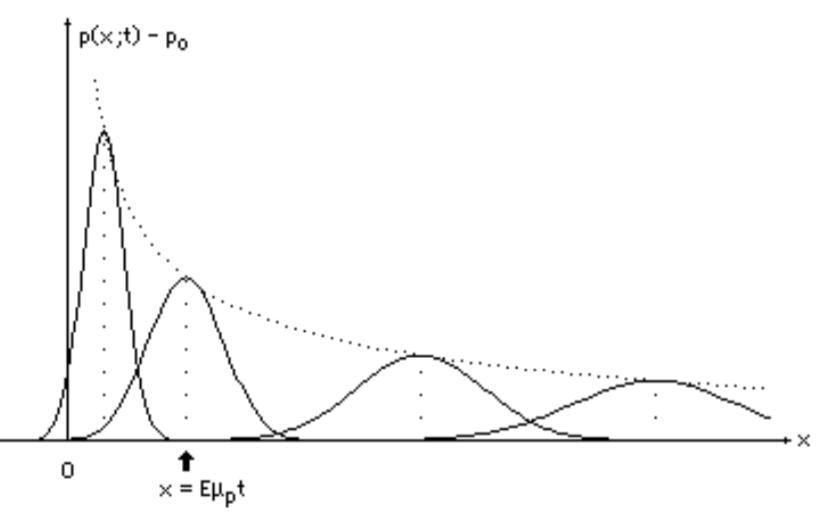
\includegraphics[width=0.6\textwidth]{Pulse2.PNG}
    \caption{Distribution de porteurs à génération constante avec champ électrique}
    \label{fig:pulse2}
\end{figure}
Les écpérience de Haynes et Schockley étaient basé sur ce principe. La détection à la poxition $x$ du maximum permettait de trouver la mobilité et la durée de vie des porteurs minoritaires.
\section{Jonction PN}
Il s'agit de la jonction de deux semiconducteurs dopés de type N et P dopé $N_D(x)$ et $N_A(x)$. Le dopage est abrupte mais pas carré dans la réalité, nous ferons l'hypothèse dans ce cours qu'elle l'est pour faciliter les calculs. Nous considérerons aussi que toutes les impuretés sont ionisées.
\subsection{Potentiel de contact}
Sachant que le niveau de Fermi doit être constant, un potentiel de contact se crée. Ce potentiel est donné par
\begin{equation}
E _ { F n } - E _ { F p } = q \Phi _ { o }
\end{equation}
Connaissant les potentiels d'équilibre
\begin{gather}
n _ { o } = N_D = n _ { i } e ^ { \left( E _ { F } - E _ { i o } \right) / k T } \quad,\quad p _ { o } = N_A =  n _ { i } e ^ { \left( E _ { i o } - E _ { F } \right) / k T }\\
E _ { F n } - E _ { i o } = k T \ln \left( \frac { N _ { D } } { n _ { i } } \right) \quad,\quad E _ { i o } - E _ { F p } = k T \ln \left( \frac { N _ { A } } { n _ { i } } \right) 
\end{gather}
Il apparaît une courbure de bande comme ceci
\begin{figure}[H]
    \centering
    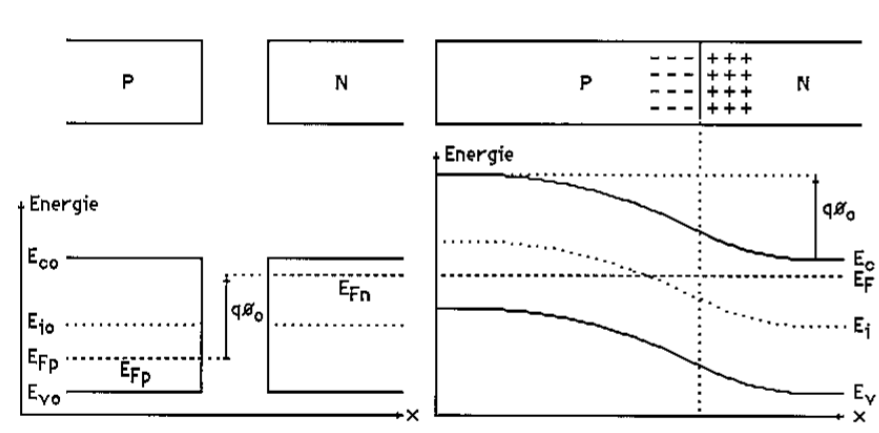
\includegraphics[width=0.6\textwidth]{Courbe2.PNG}
    \caption{Courbure de bande et potentiel de contact}
    \label{fig:curve}
\end{figure}
Le potentiel interne est
\begin{equation}
\Phi _ { o } = E _ { F n } - E _ { i o } + E _ { i o } - E _ { F p } = \frac { k T } { q } \ln \left( \frac { N _ { A } N _ { D } } { n _ { i } ^ { 2 } } \right)
\end{equation}
La présence du potentiel de contact crée des zones dépeuplées aux bords de la jonction. Cette répartition des charges crée un champ électrique. On calcule avec Poisson
\begin{equation}
\frac { d ^ { 2 } \Phi ( x ) } { d x ^ { 2 } } = - \frac { d \mathcal { E } ( x ) } { d x } = - \frac { q } { \epsilon _ { s } } \left[ p _ { o } ( x ) - n _ { o } ( x ) + N _ { D } ( x ) - N _ { A } ( x ) \right]
\end{equation}
On sait que les gradients de porteurs sont contrebalancé par le champ sur les porteurs libres. Choisissons $E_{i0} = E_F$ tel que 
\begin{gather}
n _ { o } ( x ) = n _ { i } e ^ { \left( E _ { F } - E _ { i o } \right) / k T } e ^ { q \Phi ( x ) / k T } = n _ { i } e ^ { q \Phi ( x ) / k T }\\
p _ { o } ( x ) = n _ { i } e ^ { \left( E _ { i o } - E _ { F } \right) / k T } e ^ { - q \Phi ( x ) / k T } = n _ { i } e ^ { - q \Phi ( x ) / k T }
\end{gather}
Normalement le dopage est graduel, mais puisque la zone de déplétion se trouve proche du contact on peut considérer les zones quasi-neutres comme constante. De tel manière le potentiel est bien 
\begin{equation}
\Phi _ { o } = \Phi _ { n o } - \Phi _ { p o }
\end{equation}
données par les valeurs des potentiels loin dans les bords du semiconducteur. Par l'équilibre des porteurs on a respectivement dans les zone quasi neutres P et N
\begin{gather}
p _ { p o } = N _ { A } = n _ { i } e ^ { - q \Phi _ { p o } / k T } , n _ { p o } = \frac { n _ { i } ^ { 2 } } { N _ { A } } = n _ { i } e ^ { q \Phi _ { p o } / k T }\\
p _ { n o } = \frac { n _ { i } ^ { 2 } } { N _ { D } } = n _ { i } e ^ { - q \Phi _ { n o } / k T } , n _ { n o } = N _ { D } = n _ { i } e ^ { q \Phi _ { n o } / k T }
\end{gather}
En combinant ces deux équations on trouve la relation de Boltzmann équivalente à 
\begin{equation}
\frac { p _ { p o } } { p _ { n o } } = \frac { n _ { n o } } { n _ { p o } } = e ^ { q \left( \Phi _ { n o } - \Phi _ { p o } \right) / k T } = e ^ { q \Phi _ { o } / k T } \Longleftrightarrow \Phi _ { o } = \frac { k T } { q } \ln \left( \frac { N _ { A } N _ { D } } { n _ { i } ^ { 2 } } \right)
\end{equation}
On trouve au travers de l'équation de Poisson les profils du champ électrique, des porteurs, du potentiel
\begin{figure}[H]
    \centering
    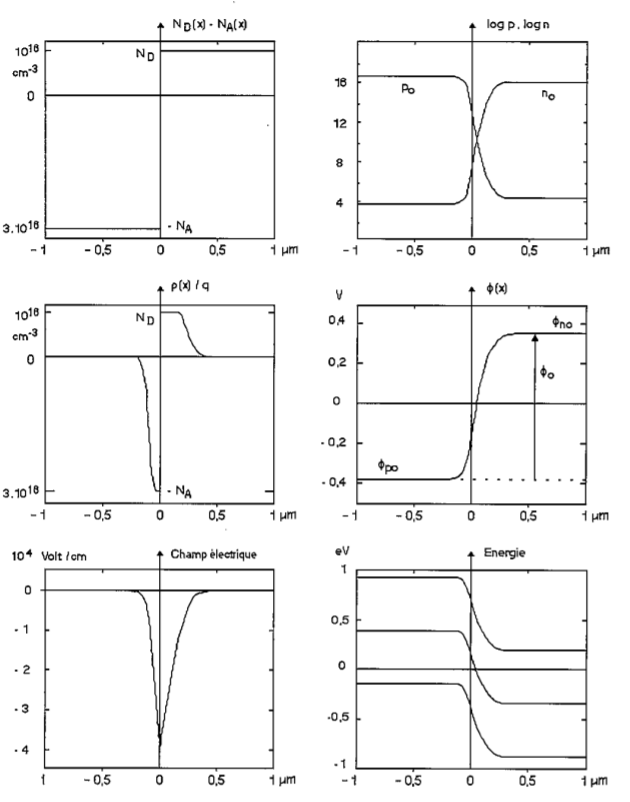
\includegraphics[width=0.6\textwidth]{Poisson.PNG}
    \caption{Profils réels obtenus par MN de Poisson à la jonction}
    \label{fig:Poisson}
\end{figure}
\subsection{Modèle de la jonction abrupte à l'équilibre}
Notre modèle sur lequel se basera la résolution contient trois zones : une zone avec une charge d'espace entourée de deux zones quasi-neutres. La zone déplété ne présente que les charges dues aux dopant ionisés. Notre modèle est donc
\begin{equation}
\rho ( x ) = \left\{ \begin{array} { c c c } { 0 } & { \text { pour } } & { - \infty < x < - l _ { p o } } \\ { - q N _ { A } } & { \text { pour } } & { - l _ { p o } < x < 0 } \\ { + q N _ { D } } & { \text { pour } } & { 0 < x < l _ { n o } } \\ { 0 } & { \text { pour } } & { l _ { n o } < x < \infty } \end{array} \right.
\end{equation}
par poisson
\begin{equation}
-\mathcal{E}= \frac { d \Phi ( x ) } { d x } = \left\{ \begin{array} { c c c } { 0 } &\text { pour } &- \infty < x < - l _ { p o } \\ { + \frac { q N _ { A } } { \epsilon _ { s } } \left( x + l _ { p o } \right) } &\text { pour } &- l _ { p o } < x < 0 \\ { - \frac { q N _ { D } } { \epsilon _ { s } } \left( x - l _ { n 0 } \right) } &\text { pour } &0 < x < l _ { n o }\\ { 0 }&\text { pour } &l _ { n o } < x < \infty \end{array} \right.
\end{equation}
et encore poisson
\begin{equation}
\Phi ( x ) = \left\{ \begin{array} { c c c } { \Phi _ { p o } } & { \text { pour } } & { - \infty < x < - l _ { p o } } \\ { \Phi _ { p o } + \frac { q N _ { A } } { 2 \epsilon _ { s } } \left( x + l _ { p o } \right) ^ { 2 } } & { \text { pour } } & { - l _ { p o } < x < 0 } \\ { \Phi _ { n o } - \frac { q N _ { D } } { 2 \epsilon _ { s } } \left( x - l _ { n o } \right) ^ { 2 } } & { \text { pour } } & { 0 < x < l _ { n o } } \\ { \Phi _ { n o } } & { \text { pour } } & { l _ { n o } < x < \infty } \end{array} \right.
\end{equation}
ce qui nous donne un profil de porteur
\begin{figure}[H]
    \centering
    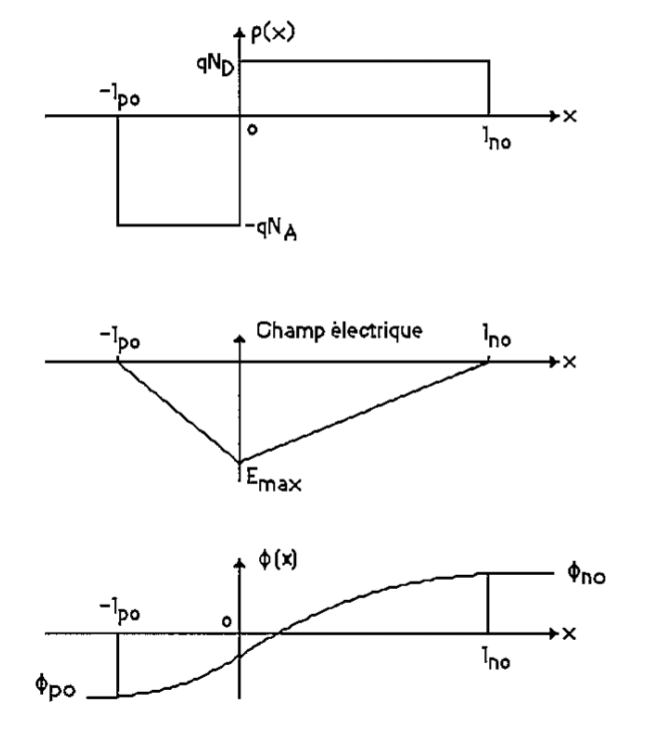
\includegraphics[width=0.6\textwidth]{Poisson2.PNG}
    \caption{Profil de porteur calculé sur base du modèle}
    \label{fig:Poisson2}
\end{figure}
Il nous faut résoudre pour trouver les longueurs de déplétion, à partir du système d'équation suivant obtenu par la continuité en $x=0$
\begin{gather}
N _ { A } l _ { p o } = N _ { D } l _ { n o }\\
\frac { q } { 2 \epsilon _ { s } } \left( N _ { A } l _ { p o } ^ { 2 } + N _ { D } l _ { n o } ^ { 2 } \right) = \Phi _ { n o } - \Phi _ { p o } = \Phi _ { o }\\
l _ { p o } = \sqrt { \frac { 2 \epsilon _ { s } } { q } \frac { \Phi _ { O } N _ { D } } { N _ { A } \left( N _ { A } + N _ { D } \right) } } , l _ { n o } = \sqrt { \frac { 2 \epsilon _ { s } } { q } \frac { \Phi _ { o } N _ { A } } { N _ { D } \left( N _ { A } + N _ { D } \right) } }
\end{gather}
On remarque les points notables suivants :
\begin{itemize}
    \item La continuité du champ impose également la neutralité de la charge
    \item Le champ maximal se situe au point $x=0$
\end{itemize}
\subsection{Jonction polarisé par une tension}
La tension modifie le potentiel de contact et le champ électrique et rompu ainsi l'équilibre. L'équilibre est donc rompu en faveur de la diffusion de porteurs libres. Le flux augmente avec la tension car il est originaire de la région peuplé en majoritaires.\\
Si la jonction est polarisé en sens inverse, la barrière de potentiel diminue et le champ électrique est augmenté. Cela bloque les courant de diffusion et augmenter les courant de dérives. Le courants de dérive sont faibles car appliqué aux minoritaires, il n'a que peut d'effet. Il existe donc un courant en sens bloquant appelé courant de saturation qui est indépendant de la tension.\\
Pour trouver ces courant il faut simultanément résoudre Poisson et les deux continuités, cela se fait par méthodes numériques.
\begin{figure}[H]
    \centering
    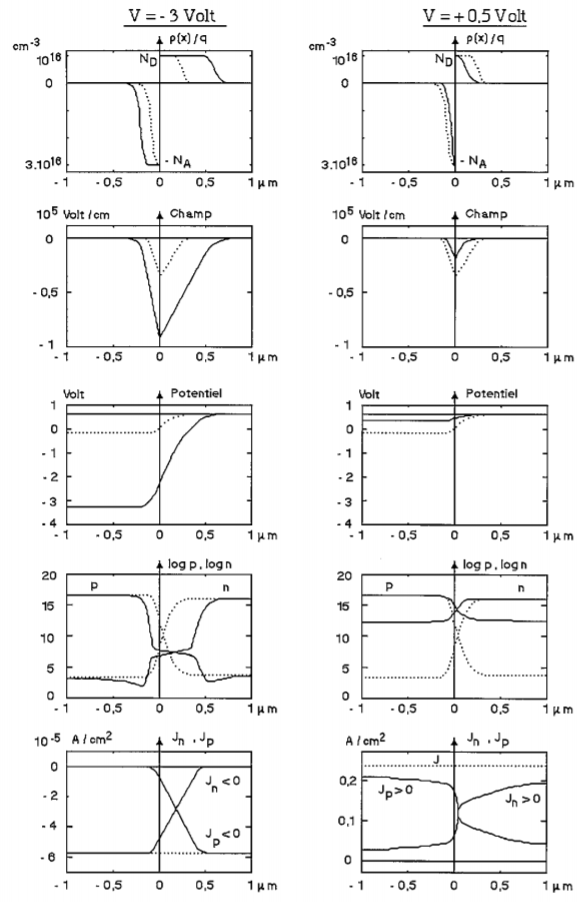
\includegraphics[width=0.6\textwidth]{PNVn0.PNG}
    \caption{Caption}
    \label{fig:exVn0}
\end{figure}
On s'aperçoit que le modèle à tension nulle est maintenu bien que les tailles des zones de déplétion sont maintenues. Il faut faire ici l'hypothèse que la tension appliquée apparaît entièrement autour de la zone de déplétion. Par les mêmes équations que précédemment 
\begin{equation}
\begin{array}{c c c}
\rho ( x ) = \left\{ \begin{array} { c } { 0 } \\ { - q N _ { A } } \\ { + q N _ { D } } \\ { 0 } \end{array} \right. \quad,& - \mathcal { E } = \frac { d \Phi ( x ) } { d x } = \left\{ \begin{array} { c } { 0 } \\ { + \frac { q N _ { A } } { \epsilon _ { s } } \left( x + l _ { p o } \right) } \\ { - \frac { q N _ { D } } { \epsilon _ { s } } \left( x - l _ { n 0 } \right) } \\ { 0 } \end{array} \right. \quad, &  \Phi ( x ) = \left\{ \begin{array} { c } { \Phi _ { p o } } \\ { \Phi _ { p o } + \frac { q N _ { A } } { 2 \epsilon _ { s } } \left( x + l _ { p o } \right) ^ { 2 } } \\ { \Phi _ { n o } - \frac { q N _ { D } } { 2 \epsilon _ { B } } \left( x - l _ { n o } \right) ^ { 2 } } \\ { \Phi _ { n o } } \end{array} \right.
\end{array}
\end{equation}
On résout pour la continuité pour trouver les longueurs de déplétion 
\begin{gather}
N _ { A } l _ { p } = N _ { D } l _ { n }\\
\frac { q } { 2 \epsilon _ { s } } \left( N _ { A } l _ { p } ^ { 2 } + N _ { D } l _ { n } ^ { 2 } \right) = \Phi _ { n } - \Phi _ { p } = \Phi _ { o } - V
\end{gather}
On trouve les expressions
\begin{equation}
l _ { p } = \sqrt { \frac { 2 \epsilon _ { s } } { q } \left( \Phi _ { o } - V \right) \frac { N _ { D } } { N _ { A } \left( N _ { A } + N _ { D } \right) } }\quad,\quad l _ { n } = \sqrt { \frac { 2 \epsilon _ { s } } { q } \left( \Phi _ { o } - V \right) \frac { N _ { A } } { N _ { D } \left( N _ { A } + N _ { D } \right) } }
\end{equation}
Ces expressions sont valables que lorsque $V < \phi _ { 0 }$.
\subsection{Calcul du courant}
Le courant est dicté par la dérive diffusion
\begin{equation}
\begin{array} { l } { J _ { n } ( x ) = q \left[ n ( x ) \mu _ { n } \mathcal { E } ( x ) + D _ { n } \frac { d n ( x ) } { d x } \right] } \\ { J _ { p } ( x ) = q \left[ p ( x ) \mu _ { p } \mathcal { E } ( x ) - D _ { p } \frac { d p ( x ) } { d x } \right] } \end{array}
\end{equation}
Il suffit de choisir un point quelconque et de calculer la densité de courant en ce point. Seulement, les approximations faites précédemment ne permettent pas de prendre un point dans la zone de déplétion. Nous ne pouvons pas non-plus prendre la densité de courant des majoritaires dans les zones quasi neutres car nous y considérons le champ électrique pratiquement nulle dans notre modèle.\\
Nous utilisons donc les porteurs minoritaires pour notre calcul, nous savons qu'il y a injection de minoriaires dans la zone quasi neutre. Cette injection se résorbe lentement par recombinaison et diffusion créant un gradient de porteur. On pourra ignorer la dérive car le produit champ-minoritaires est négligeable. \\
Soit dans les zones quasi neutres respectivement N et P
\begin{gather}
p _ { n } ( x ) - p _ { n o } \ll n _ { n 0 }\quad,\quad n _ { p } ( x ) - n _ { p o } \ll p _ { p o }\\
n _ { n o } = N _ { D } , p _ { n o } = \frac { n _ { i } ^ { 2 } } { N _ { D } } \quad,\quad p _ { p o } = N _ { A } , \quad n _ { p o } = \frac { n _ { i } ^ { 2 } } { N _ { A } }
\end{gather}
On suppose que à $V$ modéré, les rapports de grandeurs sont respectés dans les zones quasi neutres. C'est l'hypothèse de faible injection.\\
Soit la quasi-neutralité s'approxime ainsi respectivement dans N et P
\begin{gather}
n _ { n } ( x ) - n _ { n o } = p _ { n } ( x ) - p _ { n o }\\
n _ { n } ( x ) = n _ { n o } \quad,\quad p _ { p } ( x ) = p _ { p o }
\end{gather}
Les majoritaires sont constants.\\
L'hypothèse que nous avions posé était que les courant sont uniquement de la diffusion. La diffusion s'écrit
\begin{gather}
J _ { p } ( x ) = - q D _ { p } \frac { d p _ { n } ( x ) } { d x } \quad,\quad J _ { n } ( x ) = + q D _ { n } \frac { d n _ { p } ( x ) } { d x }\\
\frac { d J _ { p } } { d x } = - q U _ { p } \quad,\quad\frac { d J _ { n } } { d x } = q U _ { n }\\
D _ { p } \frac { d ^ { 2 } p _ { n } ( x ) } { d x ^ { 2 } } - U _ { p } ( x ) = 0\quad,\quad D _ { n } \frac { d ^ { 2 } n _ { p } ( x ) } { d x ^ { 2 } } - U _ { n } ( x ) = 0
\end{gather}
Nous nécessitons ici des valeurs des minoritaires aux limite de la zone de déplétion. Nous devons donc généraliser Boltzmann au cas de la tension non-nulle. Soit dans la zone de déplétion
\begin{gather}
J _ { n } ( x ) = J _ { p } ( x ) = 0\\
n \mu _ { n } \mathcal { E } ( x ) + D _ { n } \frac { d n ( x ) } { d x } = 0\quad,\quad p \mu _ { p } \mathcal { E } ( x ) - D _ { p } \frac { d p ( x ) } { d x } = 0\\
n ( x ) = n _ { n } \left( l _ { n } \right) e ^ { q \left[ \Phi ( x ) - \Phi _ { n } \right] / k T } \quad,\quad p ( x ) = p _ { p } \left( - l _ { p } \right) e ^ { - q \left[ \Phi ( x ) - \Phi _ { p } \right] / k T }\\
n ( x ) \cdot p ( x ) = n _ { n } \left( l _ { n } \right) \cdot p _ { p } \left( - l _ { p } \right) e ^ { - q \Phi _ { o } / k T } e ^ { q V / k T }\\
\Phi _ { 0 } = \frac { k T } { q } \ln \left( \frac { N _ { A } N _ { D } } { n _ { i } ^ { 2 } } \right)\\
n ( x ) \cdot p ( x ) = n _ { i } ^ { 2 } e ^ { q V / k T }
\end{gather}
On trouves finalament les relations de Boltzmann
\begin{equation}
\begin{aligned} \frac { n _ { p } \left( - l _ { p } \right) } { n _ { n } \left( l _ { n } \right) } & = e ^ { q \left( \Phi _ { o } - \Phi _ { p } \right) / k T } = e ^ { - q \left( \Phi _ { o } - V \right) / k T } = \frac { n _ { p o } } { n _ { n o } } e ^ { q V / k T } \\ \frac { p _ { n } \left( l _ { n } \right) } { p _ { p } \left( - l _ { p } \right) } & = e ^ { q \left( \Phi _ { o } - \Phi _ { p } \right) / k T } = e ^ { - q \left( \Phi _ { o } - V \right) / k T } = \frac { p _ { n o } } { p _ { p o } } e ^ { q V / k T } \end{aligned}
\end{equation}
Ce qui se réécrit plus simplement, au travers de l'hypothèse de faible injection comme 
\begin{equation}
n _ { p } \left( - l _ { p } \right) = n _ { p o } e ^ { q V / k T }\quad,\quad p _ { n } \left( l _ { n } \right) = p _ { n o } e ^ { q V / k T }
\end{equation}
Puisque les densités de courant sont calculés en des poins différents, il manque certains contributions au courant. On utilisera l'hypothèse que la recombinaison est nulle dans la zone de transition.
\begin{gather}
J = J _ { n } \left( l _ { n } \right) + J _ { p } \left( l _ { n } \right)\\
J = J _ { n } \left( - l _ { p } \right) + J _ { p } \left( l _ { n } \right) + q \int _ { - l _ { p } } ^ { l _ { n } } U _ { n } ( x ) d x\\
J = J _ { n } \left( - l _ { p } \right) + J _ { p } \left( l _ { n } \right)
\end{gather}
\subsection{Courant -Tension en régime permanent}
Listons les hypothèses émises précédemment pour le calcul des densités de courant
\begin{itemize}
    \item Il existe trois zones, une zone de transition entourée de deux ZQN (H1)
    \item La tension appliqué se retrouve entièrement aux bornes de la zone de transition (H2)
    \item L'injection dans les ZQN est faible (H3) 
    \item Les courant des porteurs minoritaires sont les courant de diffusion dans les ZQN (H4)
    \item Les relations de Boltzmann restent valables dans la zone de transition (H5)
    \item On néglige la recombinaison dans la zone de transition (H6)
\end{itemize}
Nous repartons du régime permanent dans le cas des trous pour calculer le courant
\begin{gather}
\frac { d J _ { p } } { d x } = - q U _ { p } ( x )\quad,\quad
J _ { p } ( x ) = - q D _ { p } \frac { d p _ { n } ( x ) } { d x }\quad,\quad U _ { p } ( x ) = \frac { p _ { n } ( x ) - p _ { n o } } { \tau _ { p } }\\
D _ { p } \frac { d ^ { 2 } p _ { n } ( x ) } { d x ^ { 2 } } - \frac { p _ { n } ( x ) - p _ { n 0 } } { \tau _ { p } } = 0
\end{gather}
Dont la solution est 
\begin{gather}
p _ { n } ( x ) = p _ { n o } + A e ^ { - x / L _ { p } } + B e ^ { + x / L _ { p } } \quad\text{avec}\quad L _ { p } = \sqrt { D _ { p } \tau _ { p } }
\end{gather}
Il faut lui appliquer les conditions limites, soit le retour à l'équilibre en l'infinie et la valeur en la position $0$
\begin{gather}
p _ { n } ( \infty ) = p _ { n o } \quad,\quad p(l_n) = p _ { n o } e ^ { q V / k T }
\end{gather}
On trouve ainsi la répartition des porteurs
\begin{equation}
p _ { n } ( x ) = p _ { n o } + p _ { n o } \left( e ^ { q V / k T } - 1 \right) e ^ { - \left( x - h _ { n } \right) / L _ { p } }\quad,\quad L _ { p } = \sqrt { D _ { p } \tau _ { p } }
\end{equation}
et les densités de courant (cas des électrons analogue)
\begin{gather}
J _ { p } ( x ) = \frac { q D _ { p } } { L _ { p } } p _ { n o } \left( e ^ { q V / k T } - 1 \right) e ^ { - \left( x - l _ { n } \right) / L _ { p } } \quad,\quad L _ { p } = \sqrt { D _ { p } \tau _ { p } }\\
J _ { n } ( x ) = \frac { q D _ { n } } { L _ { n } } n _ { p o } \left( e ^ { q V / k T } - 1 \right) e ^ { + \left( x + l _ { p } \right) / L _ { n } } \quad,\quad L _ { n } = \sqrt { D _ { n } \tau _ { n } }
\end{gather}
On trouve la répartition des porteurs et la densité de courant associée
\begin{figure}[H]
    \centering
    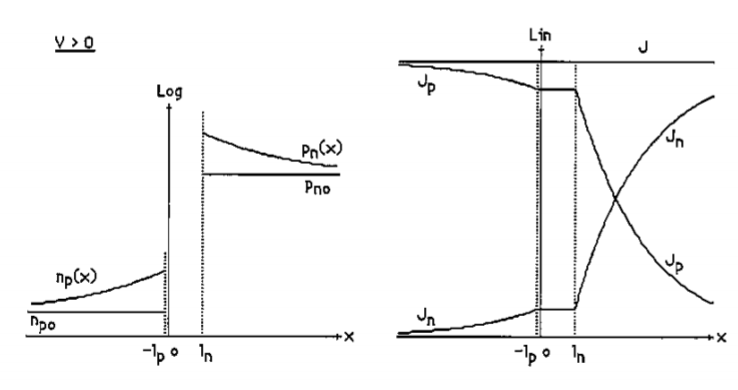
\includegraphics[width = 0.6\textwidth]{Profil.PNG}
    \caption{Profil des porteurs minoritaires}
    \label{fig:profil}
\end{figure}
Nous pouvons calculer, au travers l'hypothèse négligeant la recombinaison, la densité de courant totale
\begin{gather}
J = J _ { n } \left( - l _ { p } \right) + J _ { p } \left( l _ { n } \right)\\
J = \frac { q D _ { p } } { L _ { p } } p _ { n o } \left( e ^ { q V / k T } - 1 \right) e ^ { - \left( l_n - l _ { n } \right) / L _ { p } } + \frac { q D _ { n } } { L _ { n } } n _ { p o } \left( e ^ { q V / k T } - 1 \right) e ^ { + \left( -l_p + l _ { p } \right) / L _ { n } }\\
J = q \left( \frac { D _ { n } n _ { p o } } { L _ { n } } + \frac { D _ { p } p _ { n o } } { L _ { p } } \right)\left( e ^ { q V / k T } - 1 \right)
\end{gather}
On en extrait la densité de courant de saturation
\begin{gather}
J _ { s } = q \left( \frac { D _ { n } n _ { p o } } { L _ { n } } + \frac { D _ { p } p _ { n o } } { L _ { p } } \right) = q n _ { i } ^ { 2 } \left( \frac { 1 } { N _ { A } } \sqrt { \frac { D _ { n } } { \tau _ { n } } } + \frac { 1 } { N _ { D } } \sqrt { \frac { D _ { p } } { \tau _ { p } } } \right)
\end{gather}
Une relation intéressante est 
\begin{equation}
\frac { J _ { p } \left( l _ { n } \right) } { J _ { n } \left( - l _ { p } \right) } = \frac { L _ { n } D _ { p } } { L _ { p } D _ { n } } \frac { p _ { n o } } { n _ { p o } } = \frac { \sqrt { \mu _ { p } \tau _ { n } } } { \sqrt { \mu _ { n } \tau _ { p } } } \frac { N _ { A } } { N _ { D } }
\end{equation}
On voit immédiatement qu'en sens bloquant, dans la zone avant le claquage, la diode a un courant très faible
\begin{gather}
J = J _ { s } e ^ { q V / k T } \text { pour } V \gg k T / q\\
J = - J _ { s } \text { pour } V \ll - k T / q
\end{gather}
La valeur de $J_s$ dépend de linéairement de la concentration intrinsèque $n _ { i } ^ { 2 } \sim e ^ { - E _ { g } / k T }$, c'est de cette manière qu'on distingue les dispositifs de puissance des dispositifs analogiques.\\
Une diode idéale se doit d'avoir une densité de courant de saturation très faible , donc une concentration intrinsèque faible et avec des durées de vie les plus grandes possible.\\
Les équations de $J_s$ peuvent être simplifiés lors de dopages asymétrique (au moins deux ordres de grandeurs). Imaginons une diode $  { P } ^ { + }   { N }$, alors
\begin{gather}
p _ { n 0 } \gg n _ { p o } \Rightarrow J _ { p } \left( l _ { n } \right) \gg J _ { n } \left( - l _ { p } \right)\\
J \approx J _ { p } \left( l _ { n } \right) = \frac { q n _ { i } ^ { 2 } } { N _ { D } } \sqrt { \frac { D _ { p } } { \tau _ { p } } } \left( e ^ { q V / k T } - 1 \right)
\end{gather}
\subsection{Courant de génération recombinaison}
L'hypothèse qu'il n'y a pas de génération ni recombinaison dans la zone de transition doit être analysée à posteriori. Repartons de la continuité
\begin{gather}
\frac { d J _ { n } ( x ) } { d x } = q U _ { n } ( x ) , \frac { d J _ { p } ( x ) } { d x } = - q U _ { p } ( x )\\
J = J _ { n } + J _ { p } = CST \Rightarrow U _ { n } = U _ { p } = U
\end{gather}
La densité de courant en prenant en compte la recombinaison (chaque densité calculé dans l'autre zone quasi neutre) est 
\begin{gather}
J _ { n } \left( l _ { n } \right) = J _ { n } \left( - l _ { p } \right) + q \int _ { - l _ { p } } ^ { l _ { n } } U ( x ) d x\\
J = J _ { p } \left( l _ { n } \right) + J _ { n } \left( - l _ { p } \right) + q \int _ { - l _ { p } } ^ { l _ { n } } U ( x ) d x\\
J = J _ { s } \left( e ^ { q V / k T } - 1 \right) + J _ { r , g } \\
J _ { r , g } = q \int _ { - l _ { p } } ^ { l _ { n } } U ( x ) d x
\end{gather}
on en dégage le courant de génération recombinaison. On considérant la recombinaison pour des centres recombinant du type Schockley-Read-Hall
\begin{gather}
U ( x ) = \frac { p \cdot n - n _ { i } ^ { 2 } } { \tau _ { p o } \left( n + n _ { i } \right) + \tau _ { n o } \left( p + n _ { i } \right) }\\
\tau = \tau _ { p o } = \tau _ { n o } \Rightarrow U ( x ) = \frac { p \cdot n - n _ { i } ^ { 2 } } { \tau \left( n + p + 2 n _ { i } \right) }
\end{gather}
Dans la zone de transition, par les relations de Boltzmann (H5), on développe
\begin{gather}
p ( x ) . n ( x ) = n _ { i } ^ { 2 } e ^ { q V / k T } \quad,\quad U(x) = \frac {n _ { i } ^ { 2 } \left( e ^ { q V / k T } - 1 \right)} { \tau \left( n + p + 2 n _ { i } \right) }\\
J _ { r , g } = \frac { 1 } { \tau } q n _ { i } ^ { 2 } \left( e ^ { q V / k T } - 1 \right) \int _ { - l _ { p } } ^ { l _ { n } } \frac { d x } { n ( x ) + p ( x ) + 2 n _ { i } }
\end{gather}
À tension positive la recombinaison dans la zone de transition des porteur libre injectés par les zones quasi neutre vient s'ajouter sur la densité de minoritaires et augmentant le gradient. La densité de courant de recombinaison vient s'ajouter aux densités de courant.\\
À tension négative, la concentration de porteur libre est inférieure à l'équilibre. Les centres recombinants génèrent des paires de porteurs libres qui sont dissociés et injectés dans leurs zones respectives créant un courant négatif.\\
On tentera de borner le courant de recombinaison, soit le point particulier d'égalité $n=p$
\begin{gather}
p = n = n _ { i } e ^ { q V / 2 k T }\\
J _ { r , g } = \frac { q n _ { i } } { 2 \tau } \frac { e ^ { q V / k T } - 1 } { e ^ { q V / 2 k T } + 1 } \int _ { - l _ { p } } ^ { l _ { n } } d x\\
l _ { n } + l _ { p } = \sqrt { \frac { 2 \epsilon _ { s } } { q } \left( \Phi _ { o } - V \right) \frac { N _ { A } + N _ { D } } { N _ { A } N _ { D } } }\\
J _ { r , g } = \frac { q n _ { i } } { 2 \tau } \left( e ^ { q V / 2 k T } - 1 \right) \sqrt { \frac { 2 \epsilon _ { s } } { q } \left( \Phi _ { o } - V \right) \frac { N _ { A } + N _ { D } } { N _ { A } N _ { D } } }\\
J _ { r , g } = J _ { s , r , g } \left( e ^ { q V / 2 k T } - 1 \right) \quad,\quad J _ { s , r , g } = \frac { q n _ { i } } { 2 \tau } \sqrt { \frac { 2 \epsilon _ { s } } { q } \left( \Phi _ { o } - V \right) \frac { N _ { A } + N _ { D } } { N _ { A } N _ { D } } }
\end{gather}
La densité de courant total vaut donc
\begin{equation}
J = J_s\left( e ^ { q V /k T } - 1 \right) + J _ { s , r , g } \left( e ^ { q V / 2 k T } - 1 \right)
\end{equation}
Notons que $J _ { s , r , g } \gg J _ { s }$ et donc que le courant de génération recombinaison domine dans les basses tensions et les tensions négatives. Il faut également prendre en compte la température pour s'assurer d(utiliser le bon modèle physique.
\subsection{Multiplication de porteurs et claquage}
Le claquage est un phénomène en cas  de tension bloquante intense engendrant un courant intense. Le claquage ne détruit pas la diode bien que le courant peut. Il existe deux phénomènes à la base du claquage : l'effet Zener et l'effet d'avalanche.
\subsubsection{Claquage par avalanche}
À haute tension bloquante, la zone de transition augmente en taille, le champ électrique y est très intense et accélère les porteurs libres. Si leur énergie cinétique est suffisante, il peuvent briser les liens covalents créent des paires électrons trou, contribuant ainsi à l'effet d'avalanche.\\
Soit les coefficients d'ionisation, il s'agit du nombre de paires créer par porteur par distance parcouru.
\begin{equation}
\alpha _ { n } = \alpha _ { n , \infty } e ^ { - b _ { n } / | \mathcal { L } | } \quad,\quad \alpha _ { p } = \alpha _ { p , \infty } e ^ { - b _ { p } / | \mathcal { L } | }
\end{equation}
C'est un mécanisme de création de porteur, il contribue donc à l'équation de continuité, et ce par paire
\begin{gather}
\frac { d J _ { n } ( x ) } { d x } = + \alpha _ { n } J _ { n } ( x ) + \alpha _ { p } J _ { p } ( x ) + q U ( x )\quad,\quad\frac { d J _ { p } ( x ) } { d x } = - \alpha _ { n } J _ { n } ( x ) - \alpha _ { p } J _ { p } ( x ) - q U ( x )\\
J = J _ { n } ( x ) + J _ { p } ( x ) \quad , \quad \alpha _ { n p } = \alpha _ { n } - \alpha _ { p }\\
\frac { d J _ { n } ( x ) } { d x } - \alpha _ { n p } J _ { n } ( x ) = + \alpha _ { p } J + q U ( x ) \quad,\quad \frac { d J _ { p } ( x ) } { d x } - \alpha _ { n p } J _ { p } ( x ) = - \alpha _ { n } J - q U ( x )\\
J _ { n } \left( - l _ { p } \right) = \frac { q D _ { n } } { L _ { n } } n _ { p o } \left( e ^ { q V / k T } - 1 \right) \quad , \quad J _ { p } \left( l _ { n } \right) = \frac { q D _ { p } } { L _ { p } } p _ { n o } \left( e ^ { q V / k T } - 1 \right)
\end{gather}
La solution de ces équations est 
\begin{gather}
J _ { n } ( x ) = e ^ { \int _ { - l _ { p } } ^ { x } \alpha _ { n p } d x } \left[ J _ { n } \left( - l _ { p } \right) + J \int _ { - l _ { p } } ^ { x } \alpha _ { p } e ^ { - \int _ { - l p } ^ { x } \alpha _ { n p } d x } d x + q \int _ { - l _ { p } } ^ { x } U e ^ { - \int _ { - l _ { p } } ^ { x } \alpha _ { n p } d x } d x \right]\\
J _ { p } ( x ) = e ^ { - \int _ { x } ^ { l n } \alpha _ { n p } d x } \left[ J _ { p } \left( l _ { n } \right) + J \int _ { x } ^ { l _ { n } } \alpha _ { n } e ^ { \int _ { x } ^ { l _ { n } } \alpha _ { n p } d x } d x + q \int _ { x } ^ { l _ { n } } U e ^ { \int _ { x } ^ { l _ { n } } \alpha _ { n p } d x } d x \right]
\end{gather}
On combine pour la densité de courant total 
\begin{gather}
J = J _ { n } \left( l _ { n } \right) + J _ { p } \left( l _ { n } \right) = J _ { n } \left( - l _ { p } \right) + J _ { p } \left( - l _ { p } \right)\\
J = J _ { n } \left( l _ { n } \right) + J _ { p } \left( l _ { n } \right) = J _ { n } \left( - l _ { p } \right) + J _ { p } \left( - l _ { p } \right)\\
\end{gather}
Les expressions complètes sont
\begin{gather}
J = \frac{J _ { n } \left( - l _ { p } \right) + J _ { p } \left( l _ { n } \right) e ^ { - \int _ { - l _ { p } } ^ { l n } \alpha _ { n p } d x } + q \int _ { - l _ { p } } ^ { l _ { n } } U e ^ { - \int _ { - l _ { p } } ^ { x } \alpha _ { n p } d x } d x}{1 - \int _ { - l _ { p } } ^ { l _ { n } } \alpha _ { n } e ^ { - \int _ { - l _ { p } } ^ { x } \alpha _ { n p } d x } d x}\\
J = \frac{J _ { n } \left( - l _ { p } \right) e ^ { \int _ { - l _ { p } } ^ { l n } \alpha _ { n p } d x } + J _ { p } \left( l _ { n } \right) + q \int _ { - l _ { p } } ^ { l _ { n } } U e ^ { \int _ { x } ^ { l _ { n } } \alpha _ { n p } d x } d x}{1 - \int _ { - l _ { p } } ^ { l _ { n } } \alpha _ { p } e ^ { \int _ { x } ^ { l n } \alpha _ { n p } d x } d x}
\end{gather}
Soit un facteur multiplicatif du courant en cas d'avalanche
\begin{gather}
M = \frac { J } { J ^ { * } } ( \geq 1 )\\
M \rightarrow \infty \Rightarrow \mathbf { 1 } = \int _ { - l _ { p } } ^ { l _ { n } } \alpha _ { n } e ^ { - \int _ { - l _ { p } } ^ { x } \alpha _ { n p } d x } d x \quad \text{ou} \quad 1 = \int _ { - l _ { p } } ^ { l _ { n } } \alpha _ { p } e ^ { \int _ { x } ^ { l _ { n } } \alpha _ { n p } d x } d x\\
\end{gather}
On simplifie
\begin{gather}
\frac { \alpha _ { p } } { \alpha _ { n } } = \gamma\\
1 = \int _ { - l _ { p } } ^ { l _ { n } } \alpha _ { n } e ^ { - ( 1 - \gamma ) \int _ { - l _ { p } } ^ { x } \alpha _ { n } d x } d x\\
1 = \frac { 1 } { 1 - \gamma } \left[ 1 - e ^ { - ( 1 - \gamma ) \int _ { - l _ { p } } ^ { l _ { n } } \alpha _ { n } d x } \right]\\
\int _ { - l _ { p } } ^ { l _ { n } } \alpha _ { n } d x = \frac { \ln ( y ) } { \gamma - 1 }
\end{gather}
Soit les coefficients effectifs d'ionisation définit comme suit
\begin{gather}
\alpha _ { e f f } = \alpha _ { n } \frac { \gamma - 1 } { \ln ( y ) } \text { soit } \alpha _ { e f f } = \alpha _ { \infty } e ^ { - b _ { n } / | \mathcal { E } | }
\end{gather}
et enfin la condition d'avalanche
\begin{equation}
\int _ { - l _ { p } } ^ { l _ { n } } \alpha _ { e f f } d x = 1
\end{equation}
On remarque la relation à la tension grâce aux longueurs de déplétion, et la relation au champ électrique à l'intérieur de la zone de déplétion dans le coefficient. La tension d'avalanche est aussi liée à la température au travers de la diminution du libre parcours moyen avec les vibrations de réseau.\\
Formule empirique du facteur de multiplication en fonction de la tension de claquage $V_B$
\begin{equation}
M = \frac { J } { J ^ { * } } = \frac { 1 } { 1 - \left( \left| \frac { V } { V _ { B } } \right| \right) ^ { n } } \quad ( 3 < n < 7 )
\end{equation}
\subsubsection{Claquage par avalanche d'une jonction abrupte}
Soit une jonction $P ^ { + } N$, on peut donc simplifier la longueur de la zone de transition. Au point du champ maximum on a $x=0$
\begin{gather}
l _ { n } = \sqrt { \frac { 2 \epsilon _ { s } } { q N _ { D } } \left( \Phi _ { o } - V \right) } , \quad \mathcal { E } _ { \max } = \mathcal { E } ( 0 ) = - \sqrt { \frac { 2 q } { \epsilon _ { s } } \left( \Phi _ { o } - V \right) N _ { D } }\\
\mathcal { E } ( x ) = \mathcal { E } _ { \max } \left( 1 - \frac { x } { l _ { n } } \right) \quad , \quad L _ { n } = - \frac { \epsilon _ { s } \mathcal { E } _ { \max } } { q N _ { D } } , \quad L _ { p } = 0
\end{gather}
On a donc des expressions simples à manipuler. La condition d'avalanche est alors
\begin{gather}
1 = \int _ { 0 } ^ { l _ { n } } \alpha _ { e f f } d x = \int _ { 0 } ^ { l _ { n } } \alpha _ { \infty } e ^ { - b _ { n } / | \mathcal { E } ( x ) | } d x
\end{gather}
Grâce à l'approximation suivante on écrit
\begin{gather}
\frac { 1 } { 1 - \frac { x } { l _ { n } } } \approx 1 + \frac { x } { l _ { n } }\\
1 = \int _ { 0 } ^ { l _ { n } } \alpha _ { \infty } e ^ { - \frac { b } { \mathcal { E}_{max } } \left( 1 + \frac { x } { l _ { n } } \right) } d x\\
1 = \alpha _ { \infty } \mathcal { E } _ { \max } ^ { 2 } \frac { \epsilon _ { s } } { q N _ { D } b } e ^ { - b / \left| \mathcal { E } _ { \max } \right| } \left( 1 - e ^ { - b / \left| \mathcal { E } _ { \max } \right| } \right)
\end{gather}
On trouve ainsi la valeur critique de la tension
\begin{equation}
V _ { B } = \Phi _ { o } - \frac { \epsilon _ { s } } { 2 q N _ { D } } \mathcal { E } _ { \max } ^ { 2 }
\end{equation}
\subsubsection{Claquage par effet Zener}
Si à haute tension le claquage par avalanche ne se produit pas, un autre effet peut apparaître bien avant. La haute tension peut rompre les liens covalents dont les électrons migrent alors par effet tunnel dans la bande de conduction.
\begin{figure}[H]
    \centering
    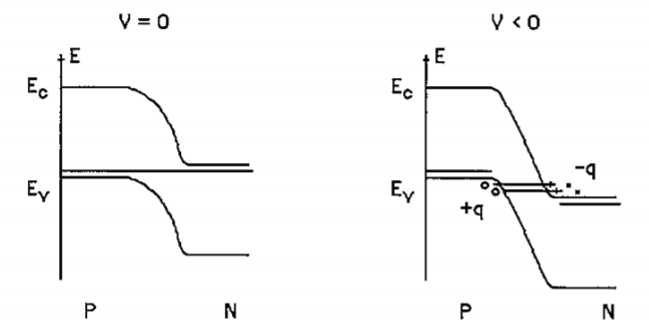
\includegraphics[width=0.6\textwidth]{Zener.PNG}
    \caption{Transition par effet tunnel des électrons de la bande de valence dans la bande de conduction}
    \label{fig:zener}
\end{figure}
Pour que ce phénomène apparaisse, le champ local doit être très grand, et donc le dopage également. Les tension sont en général très faibles pour ce phénomène $\approx 10V$.
\subsection{Effet de la température}
Développons pour mettre en évidence l'effet de la température
\begin{gather}
I = I _ { s } \left( e ^ { q V / k T } - 1 \right)\\
n _ { i } ^ { 2 } \sim T ^ { 3 } \cdot e ^ { - E _ { g } / k T }\\
n _ { i } ^ { 2 } ( T ) = n _ { i } ^ { 2 } \left( T _ { o } \right) \cdot e ^ { a \left( T - T _ { o } \right) }
\end{gather}
On utilise un rapport pour générer la relation avec la température, la valeur de $a$ dépend du matériau.\\
Dans la zone de validité de l'hypothèse qu'il n'y a pas de recombinaison dans la zone de transition on a
\begin{gather}
V = \frac{kT}{q} \ln \left( \frac{I}{I_s} \right)\\
\left( \frac { d V } { d T } \right) _ { I = CST } = \frac { V } { T } - \frac { k T } { q } \frac { d \ln \left( I _ { s } \right) } { d T } = \frac { V } { T } - \frac { k T } { q } a
\end{gather}
Le second terme surpasse le premier, donc la tension à courant constant est moindre à plus haute température. Dans le cas de la zone ou le courant de recombinaison domine, celui ci 
\begin{gather}
I _ { s , r , g } \sim n_i(T)\\
\frac{dV}{dT}\vert_{V \ll \frac{-kT}{q}} \approx 2\frac{dV}{dT}\vert_{V \gg \frac{-kT}{q}}
\end{gather}
\subsection{Capacité de transition d'une jonction abrupte}
En fonctionnement dynamique, la diode voit sa tension changer rapidement, et donc ses longueur de déplétion. On approxime la charge devant bouger sous la forme d'un volume de charge
\begin{gather}
  { l } _ {   { p } } = \sqrt { \frac { 2 \varepsilon _ {   { s } } } {   { q } } \frac { \phi   { N } _ {   { D } } } {   { N } _ {   { A } } \left(   { N } _ {   { A } } +   { N } _ {   { D } } \right) } } \quad , \quad 1 _ {   { n } } = \sqrt { \frac { 2 \varepsilon _ {   { s } } } {   { q } } \frac { \phi   { N } _ {   { A } } } {   { N } _ {   { D } \left(   { N } _ {   { A } } +   { N } _ {   { D } } \right) } } }\\
  w _ { D } = l _ { n } + l _ { p } = \sqrt { \frac { 2 \varepsilon _ { s } \phi _ { 0 } } { q } } \sqrt { \frac { N _ { A } + N _ { D } } { N _ { A } N _ { D } } } \sqrt { \frac { \phi _ { 0 } - V _ { D } } { \phi _ { 0 } } }\\
  C _ { d e p l } = \varepsilon _ { s } \frac { A } { w _ { D } }
\end{gather}



% \begin{equation}
% Q _ { j } = A q N _ { D } l _ { n } = A q N _ { A } l _ { p }
% \end{equation}
% Ce déplacement de charges abruptes donne un effet capacitif
% \begin{equation}
% C _ { T } = \lim _ { \Delta V \rightarrow 0 } \left| \frac { \Delta Q _ { j } } { \Delta V } \right| = \left| \frac { d Q _ { j } } { d V } \right|
% \end{equation}
% La constante de temps est le temps de relaxation diélectrique $\epsilon_s/\sigma$. C'est équivalent à calculer le courant de déplacement lié à la variation du champ électrique
% \begin{gather}
% \overline { D } = \epsilon _ { s } \overline { \mathcal { E } }\\
% I = A \epsilon _ { s } \frac { \partial \mathcal { E } ( x ) } { \partial t }\\
% \mathcal { E } ( x ) = \frac { q N _ { D } } { \epsilon _ { s } } \left( x - l _ { n } \right) \quad\text{pour}\quad 0 \leq x \leq l _ { n }\\
% I = - A q N _ { D } \frac { d l _ { n } } { d t } = - A q N _ { D } \frac { d l _ { ln } } { d V } \frac { d V } { d t } = - \frac { d Q _ { J } } { d V } \frac { d V } { d t } = -C_T\frac{dV}{dT}\\
% C_T = -A q N _ { D } \frac { d l _ { l n } } { d V }\\
% l _ { n } = \sqrt { \frac { 2 \epsilon _ { s } } { q } \left( \Phi _ { o } - V \right) \frac { N _ { A } } { N _ { D } \left( N _ { A } + N _ { D } \right) } }\\
% Q _ { j } =A \sqrt { 2\epsilon _ { s } q \frac { N _ { A } N _ { D } } { N _ { A } + N _ { D } } } \sqrt { \Phi _ { o } - V } \Rightarrow  \frac{dQ_j}{dV} = A \sqrt { 2\epsilon _ { s } q \frac { N _ { A } N _ { D } } { N _ { A } + N _ { D } } } \frac{-1}{\sqrt { 4\Phi _ { o } - V } }\\
% C _ { T } = \frac { A \sqrt { \frac { \epsilon _ { s } q } { 2 } \frac { N _ { A } N _ { D } } { N _ { A } + N _ { D } } } } { \sqrt { \Phi _ { o } - V } } \quad\text { ou }\quad C _ { T } = \frac { A \epsilon _ { s } } { l _ { n } + l _ { p } }
% \end{gather}

\subsubsection{Variation pour les jonctions au dopage graduel}
Une diode à jonction linéaire verra le degré de sa capacité de déplétion sous la racine du degré de la fonction de son dopage. Cela vietn du fait que poisson intègre, donc un dopage linéaire a une tension de degré $3$, donc une capacité de degré $1/3$.
\begin{equation}
C _ { j } = \frac { C _ { j 0 } } { \left( 1 - V _ { D } / \phi _ { 0 } \right) ^ { m } }
\end{equation}
avec $C_{j0}$ la capacité sous tension nulle.
\subsection{Capacité de diffusion}
La charge stocké dans les régions quasi-neutres varie également avec la variation des tailles des zones de déplétion. On appelle ça la charge de diffusion. Soit les charges associées aux tailles des zones de diffusion
\begin{gather}
I = \frac {   { dQ } } {   { dt } } = \frac {   { dQ } } {   { dV } }  \frac {   { d }   { V } } {   { dt } } =   { C } _ {   { diff } } \frac {   { d }   { V } } {   { dt } }\\
  { Q } =   { Q } _ {   { nP } } +   { Q } _ {   { pN } } \Rightarrow C _ { \text { diff } } = \frac { d Q _ { n P } } { d V } + \frac { d Q _ { p N } } { d V }
\end{gather}
Si on ne prend pas en compte la variation des zonnes de déplétion et uniquement des gradients on a 
\begin{gather}
\frac {   { d }   { Q } _ {   { nP } } } {   { dV } } = \frac {   { d } } {   { d }   { V } } \left[Q _ {   { nP0 } } \left(   { e } ^ { \frac {   { V } _ {   { D } } } { \phi _ {   { T } } } } - 1 \right)\right] = \frac { Q _ { n P 0 } } { \phi _ { T } } \left( e ^ { \frac { v _ { 0 } } { \phi _ { T } } } \right) = \frac { Q _ { \text { np } } } { \phi _ {   { T } } }
\end{gather}
La capacité est donc donnée par 
\begin{gather}
C_{diff} = \frac { Q _ { n P } + Q _ { p N } } { \phi _ { T } }\\
C_{diff} = \frac { A q } { 2 \phi _ { T } } \frac { V _ { D } } { e ^ { \phi _ { T } } }\left[ w _ { p } n _ { p 0 } + w _ { N } p _ { n 0 } \right]
\end{gather}
attention, dans le cas d'une diode longue il faut remplacer $w_p$ par $L_p$.\\
L'équation du modèle complet est
\begin{equation}
l _ { D _ {   { tot } } } = I _ {   { s } }\left[e ^ { \frac { V _ { D } } { \phi _ { T } } } - 1\right]+ C \left( V _ { D } \right) \frac { d V _ { D } } { d t }
\end{equation}
\subsection{Modèle petit signal}
On construit le modèle petit signal sur une linéarisation par taylor autour d'un point de fonctionnement. Soit la linéarisassions du courant autour de $V_0 + v$
\begin{gather}
I(V) = I _ { s } \left[ e ^ { \frac { V _ { D } } { \phi _ { T } } } - 1 \right] = I_0 + i(v)\\
g_0 = \frac{dI}{dV}\vert_{V=V_0} = \frac{I _ { s } e ^ { \frac {V _ { 0 } } { \phi _ { T } } } }{\phi_T} = \frac{I_0+I_s}{\phi_T} \Rightarrow r_0 = \frac{1}{g_0}
\end{gather}
\subsection{Photodiode}
Il s'agit d'une diode dont l'illumination dans la zone de déplétion provoque la générationd de paires électron trous. Sous l'influence du champ électrique celles-ci vont migrer dans leurs zones respectives. La génération est somme directe au courant
\begin{gather}
G ( x ) = \alpha \varphi _ { 0 } e ^ { - \alpha x }\\
J = J_0\left(e^\frac{qV}{kT}-1\right) - J_L\\
J_L = q G \left[ W + L _ { e } + L _ { h } \right]
\end{gather}
Les zones de déplétion doivent rejoindre au moins un contact pour que la génération se fasse dans la bonne zone.

\section{Transistor Bipolaire}
Le transistor est composé d'une jonction NPN (PNP) avec un accès à chaque dopage. Chaque accès porte un nom : Base, Collecteur et Émetteur, chacun se distingue par son initiale. On définit les sens des courants et tensions comme entrant. L'émetteur et le collecteur peuvent être symétriques mais se distinguent en général par leur dopages.
\begin{figure}[H]
    \centering
    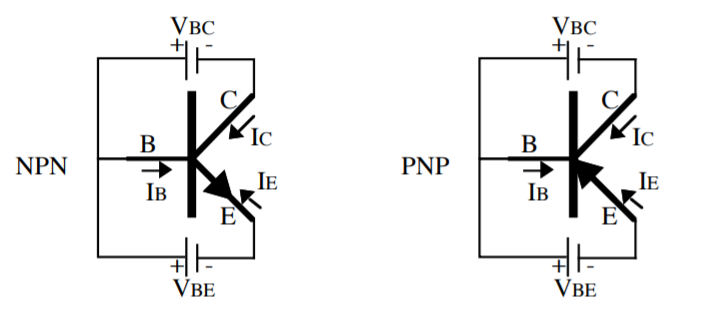
\includegraphics[width = 0.6\textwidth]{BJT.PNG}
    \caption{Définitions des sens des accès du transistor BJT}
    \label{fig:BJT}
\end{figure}
\subsection{Base longue et base courte}
Dans le cas d'une base longue, On peut considérer le BJT comme une jonction de deux diodes puisque la longueur de la base implique que les minoritaires et majoritaires retournent à l'équilibre avant de rejoindre la zone de déplétion.\\
Dans le cas d'une base mince, les minoritaires n'ont pas le temps de se recombiner intégralement. Il reste don un surplus important d'électrons qui va diffuser jusqu'à la zone de déplétion et être aspiré par la zone de déplétion suivante. Le courant E-C est donc très important et le courant de base est très faible puisque la recombinaison est faible.
\subsection{Régimes du transistor}
\begin{figure}[H]
    \centering
    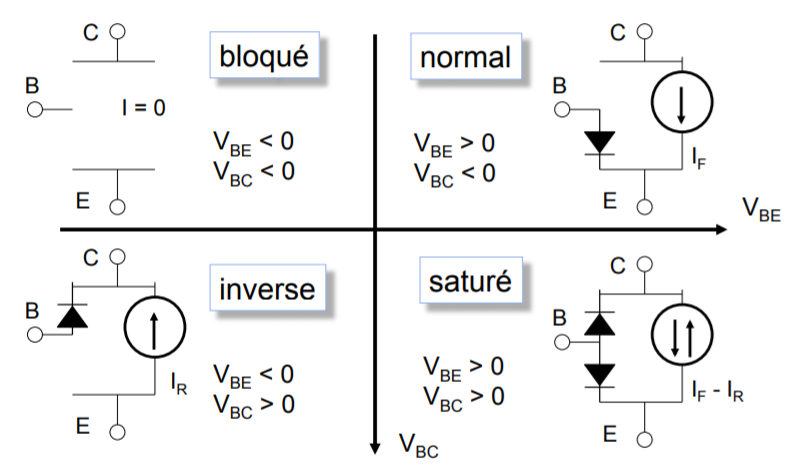
\includegraphics[width=0.7\textwidth]{Regime}
    \caption{Régimes de fonctionnement en fonction des tensions appliqué}
\end{figure}
\begin{figure}[H]
    \centering
    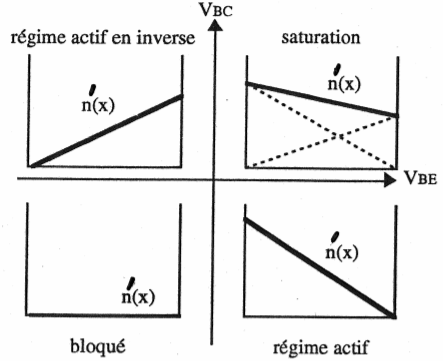
\includegraphics[angle=1,width=0.6\textwidth]{base}
    \caption{Distribution des minoritaires dans la base selon le régime}
\end{figure}
\textbf{Bloqué :} Les deux diodes sont polarisées en sens bloquant. Seul le courant de fuite passe.\\
\textbf{Actif inverse :} Les deux diodes sont passante mais le collecteur a la plus haute tension. Le courant traverse le transistor inverse. Ce régime est un régime actif de mauvaise qualité car le dopage asymétrique rend le $\beta$ très mauvais.\\
\textbf{Régime actif :} La tension de l'émetteur est la plus haute. Les jonctions sont passantes et le $\beta$ est grand.\\
\textbf{Régime saturé :} la différence de tension entre le collecteur et l'émetteur n'est pas notable. Le courant ne dépend que peu de la tension $V_{BE}$. Les électrons sont injectés dans l'émetteur et le collecteur et se recombinent dans la base.
\subsection{Modèle d'Ebers et Moll}
Nous repartons sur base des hypothèses faites dans le cadre de la jonction PN. On calcule d'abord les densités de courant de chaque jonction soi
\begin{gather}
\begin{aligned}   { I } _ {   { E } } = &   { A } \left(   { J } _ {   { pE } } +   { J } _ {   { nE } } \right) \\   { I } _ {   { C } } = & -   { A } \left(   { J } _ {   { pC } } +   { J } _ {   { n }   { C } } \right) \end{aligned}
\end{gather}
Par Boltzmann, nous calculons la concentration de minoritaires
\begin{gather}
\begin{array} { l } {   { p } _ {   { E } } ^ { \prime } (   { x } ) =   { p } _ {   { oE } } \left[ \exp \left( \frac{  { qV } _ {   { BE } }}{  { kT }} \right) - 1 \right] \exp \left[ \frac{\left(   { x } - l _ {   { E } 1 } \right)}{  { L } _ {   { pE } }} \right] } \quad,\quad   { p } _ {   { oE } } =   { n } _ {   { i } } ^ { 2 } /   { N } _ {   { DE } }\\
{   { p } _ {   { C } } ^ { \prime } (   { x } ) =   { p } _ {   { oc } } \left[ \exp \left( \frac{  { qV } _ {   { BC } }}{  { kT }} \right) - 1 \right] \exp \left[ \frac{- \left(   { x } - l _ {   { C } 2 } \right)}{   { L } _ {   { pC } }} \right] }\quad,\quad   { P } _ {   { oC } } =   { n } _ {   { i } } ^ { 2 } /   { N } _ {   { DC } } \end{array}
\end{gather}
On calcule la dérive dans le collecteur et l'émetteur
\begin{gather}
  { J } _ {   { pE } } = -   { qD } _ {   { pE } } \left. \frac {   { d }   { p } } {   { dx } } \right| _ {   { X } =   { l } _ {   { E } 1 } } = - \frac {   { qD } _ {   { pE } }p_{0E} } {   { L } _ {   { pE } } } \left[ \exp \left( \frac {   { qV } _ {   { BE } } } {   { kT } } \right) - 1 \right]\\
  { J } _ {   { pC } } = -   { qD } _ {   { pC } } \left. \frac {   { d }   { p } } {   { d }   { x } } \right| _ {   { x } =   { l } _ {   { C } 2 } }= + \frac {   { qD } _ {   { p }   { C }    } { p } _ {   { OC } } } {   { L } _ {   { pC } } } \left[ \exp \left( \frac {   { q }   { V } _ {   { BC } } } {   { kT } } \right) _ { - 1 } \right]
\end{gather}
dans le cas du collecteur, la longueur de la base ne permet pas de travailler avec le modèle de la diode immédiatement, on repart de al répartition
\begin{gather}
  { J } _ {   { n } } (   { x } ) =   { q }   { D } _ {   { nB } } \frac {   { d }   { n } } {   { d }   { x } }\\
\frac { \partial   { n } } { \partial   { t } } = \frac { 1 } {   { q } } \frac { \partial   { J } _ {   { n } } } { \partial   { x } } -   { U } = \frac { 1 } {   { q } } \frac { \partial   { J } _ {   { n } } } { \partial   { x } } - \frac {   { n } (   { x } ) -   { n } _ {   { oB } } } { \tau _ {   { nB } } } \quad,\quad   { n } _ {   { oB } } =   { n } _ {   { i } } ^ { 2 } /   { N } _ {   { AB } }
\end{gather}
Ce qui se résout en 
\begin{gather}
\frac {   { d } ^ { 2 }   { n } } {   { dx } ^ { 2 } } = \frac {   { n } (   { x } ) -   { n } _ {   { oB } } } {   { D } _ {   { nB } } \tau _ {   { nB } } } = \frac {   { n } (   { x } ) -   { n } _ {   { oB } } } {   { L } _ {   { nB } } ^ { 2 } }\\
n ( x ) = n _ { 0 B } + A \exp \left( \frac { x } { L _ { n B } } \right) + B \exp \left( \frac { - x } { L _ { n B } } \right)\quad,\quad   { L } _ {   { nB } } = \sqrt {   { D } _ {   { nB } } \tau _ {   { nB } } }\\
n(0) =  n _ { 0 B } + A + B \quad,\quad n(w_B) =  n _ { 0 B } + A \exp \left( \frac { w_B } { L _ { n B } } \right) + B \exp \left( \frac { - w_B } { L _ { n B } } \right)
\end{gather}
Grâce aux conditions limites, trouvées grâce à boltzmann on résout les constantes d'intégration
\begin{gather}
  { n } ( 0 ) =   { n } _ {   { oB } } \exp \left( \frac {   { qV } _ {   { BE } } } {   { kT } } \right) \quad,\quad   { n } \left(   { w } _ {   { B } } \right) =   { n } _ {   { oB } } \exp \left( \frac {   { qV } _ {   { BC } } } {   { kT } } \right)\\
  n^\prime ( 0 ) = n _ { o B } \left[\exp \left( \frac { q V _ { B E } } { k T } \right) - 1\right] \quad , \quad n^\prime \left( w _ { B } \right) = n _ { o B } \left[\exp \left( \frac { q V _ { B C } } { k T } \right) - 1\right]\\
  p ^ { \prime } ( l_E ) = p _ { o E } \left[\exp \left( \frac { q V _ { B E } } { k T } \right) - 1\right] \quad , \quad p ^ { \prime } \left( l_c \right) = p _ { o C } \left[\exp \left( \frac { q V _ { B C } } { k T } \right) -1\right]\\
  { n } _ {   { B } } ^ { \prime } (   { x } ) =   { n } _ {   { B } } ^ { \prime } ( 0 ) \frac { \sinh \left( \frac {   { w } _ {   { B } } -   { x } } {   { L } _ {   { nB } } } \right) } { \sinh \left( \frac {   { w } _   { B } } {   { L } _ {   { nB } } } \right) } +   { n } _ {   { B } } ^ { \prime } (   { w }   { B } ) \frac { \sinh \left( \frac {   { x } } {   { L } _ {   { nB } } } \right) } { \sinh \left( \frac {   { w } _   { B } } {   { L } _ {   { nB } } } \right) }
\end{gather}
L'évaluation de la dérivé en $x=0$ donne la densité de courant injecté dans la base, et en $x=w_b$ 
\begin{gather}
  { J } _ {   { nE } } =   { qD } _ {   { nB } } \left. \frac {   { dn } } {   { dx } } \right| _ {   { x } =   { 0 } } = - \frac {   { qD } _ {   { nB } } } {   { L } _ {   { nB } } \tanh \left( \frac {   { w } _ {   { B } } } {   { L } _ {   { nB } } } \right) }   { n }^\prime _ {   { B } } ( 0 ) + \frac {   { qD } _ {   { nB } } } {   { L } _ {   { nB } } \sinh \left( \frac {   { w } _ {   { B } } } {   { L } _ {   { nB } } } \right) }   { n }^\prime _ {   { B } } \left(   { w } _ {   { B } } \right)\\
  { J } _ {   { nC } } =   { q }   { D } _ {   { nB } } \left. \frac {   { dn } } {   { dx } } \right| _ {   { x } =   { w } _ {   { B } } } = - \frac {   { qD } _ {   { nB } } } {   { L } _ {   { nB } } \sinh \left( \frac {   { w } _ {   { B } } } {   { L } _ {   { aB } } } \right) }   { n }^\prime _ {   { B } } ( 0 ) + \frac {   { q }   { D } _ {   { aB } } } {   { L } _ {   { nB } } \tanh \left( \frac {   { w } _ {   { B } } } {   { L } _ {   { nB } } } \right) }   { n } _ {   { B } } ^ { \prime } \left(   { w } _ {   { B } } \right)
\end{gather}
il suffit alors d'injecter pour avoir l'équation complète
\begin{gather}
\begin{aligned}   { I } _ {   { E } } = &   { A } \left(   { J } _ {   { pE } } +   { J } _ {   { nE } } \right) \\   { I } _ {   { C } } = & -   { A } \left(   { J } _ {   { pC } } +   { J } _ {   { n }   { C } } \right) \end{aligned}
\end{gather}
Pour trouver les équations d'Ebers et Moll (elles sont trop longues et c'est juste un combili des équationns au dessus donc la flemme).\\
On peut à partir de ces équations facilement retrouver les gains
\begin{gather}
\alpha _ {   { F } } = - \left. \frac {   { I } _ {   { C } } } {   { I } _ {   { E } } } \right| _ {   { V } _ {   { BC } } = 0 } \quad,\quad \alpha _ {   { R } } = - \left. \frac {   { I } _ {   { E } } } {   { I } _ {   { C } } } \right| _ {   { V } _ {   { BE } } = 0 }\\
\beta _ {   { F } } = \frac { \alpha _ {   { F } } } { 1 - \alpha _ {   { F } } } \quad \text { et } \quad \beta _ {   { R } } = \frac { \alpha _ {   { R } } } { 1 - \alpha _ {   { R } } }\\
\alpha _ {   { F } } = \frac { \beta _ {   { F } } } { 1 + \beta _ {   { F } } } , \quad \frac { 1 } { \alpha _ {   { F } } } = 1 + \frac { 1 } { \beta _ {   { F } } } \quad \text { et } \quad \alpha _ {   { R } } = \frac { \beta _ {   { R } } } { 1 + \beta _ {   { R } } } , \quad \frac { 1 } { \alpha _ {   { R } } } = 1 + \frac { 1 } { \beta _ {   { R } } }
\end{gather}
Le courant de saturation s'obtient en isolant les termes en fonction de la tension
\begin{gather}
  { I } _ {   { S } } = \frac {   { AqD } _ {   { nB } }   { n } _ {   { 0B } } } {   { L } _ {   { nB } } \sinh \left( \frac {   { w } _ {   { B } } } {   { L } _ {   { nB } } } \right) }
\end{gather}
Soit les courants forward et reverse 
\begin{gather}
  { I } _ {   { F } } =   { I } _ {   { S } } \left[\exp \left( \frac { q V _ { B E } } { k T } \right) - 1\right] \quad \text { et } \quad   { I } _ {   { R } } =   { I } _ {   { S } } \left[\exp \left( \frac { q V _ { B C } } { k T } \right) - 1\right]
\end{gather}
On termine notre modèle par la relation suivante
\begin{equation}
  { I } _ {   { E } } =   { I } _ {   { R } } -   { I } _ {   { F } } - \frac {   { I } _ {   { F } } } { \beta _ {   { F } } } \quad \text { et } \quad   { I } _ {   { C } } =   { I } _ {   { F } } -   { I } _ {   { R } } - \frac {   { I } _ {   { R } } } { \beta _ {   { R } } }
\end{equation}
qui nous permet de faire le schéma suivant
\begin{figure}[H]
    \centering
    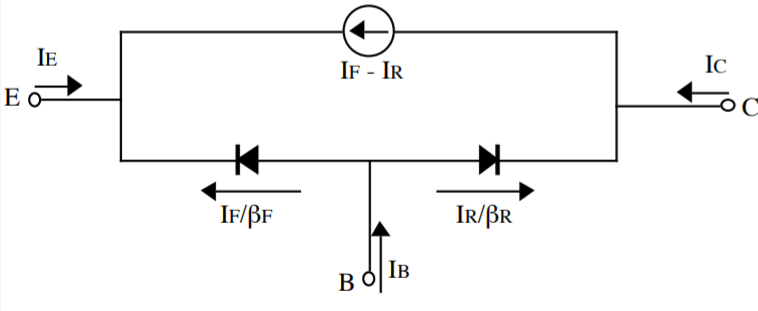
\includegraphics[width=0.6\textwidth]{EMmodel}
    \caption{Modèle d'Ebers et Moll mettant en évidence les directions des courants}
\end{figure}
\subsection{Interprétation du modèle}
Soit le rendement d'émetteur $\gamma_f$, le rapport entre le courant injecté par l'émetteur et le courant circulant entre la base et l'émetteur
\begin{gather}
\gamma _ {   { F } } = \left. \frac {   { I } _ {   { nE } } } {   { I } _ {   { nE } } +   { I } _ {   { pE } } } \right| _ {   { V }   { B }   { C } ^ { = 0 } } = \left. \frac { 1 } { 1 + \frac {   { I } _ {   { pE } } } {   { I } _ {   { nE } } } } \right| _ {   { V } _ {   { BE } } = 0 }\\
\gamma _ {   { F } } = \frac { 1 } { 1 + \frac {   { D } _ {   { pE } }   { p } _ {   { oB } }   { L } _ {   { nB } } } {   { D } _ {   { nB } }   { n } _ {   { oB } }   { L } _ {   { pE } } } \tanh \left( \frac {   { w } _ {   { B } } } {   { L } _ {   { nB } } } \right) }
\end{gather}
Soit l'approwimation de base mince $  { w } _ {   { B } } \ll   { L } _ {   { nB } }$
\begin{gather}
\gamma _ {   { F } } = \frac { 1 } { 1 + \frac {   { D } _ {   { pE } p_{oB}}   { L } _ {   { nB } } } {   { D } _ {   { nB } }   { n } _ {   { oB } }   { L } _ {   { PE } } } \frac {   { w } _ {   { B } } } {   { L } _ {   { nB } } }} = = \frac { 1 } { 1 + \frac { \mu _ {   { pE } }   { P_{oE} }   { WB } } { \mu _ {   { n }   { B } }   { n } _ {   { oB } }   { L } _ {   { pE } } } }
\end{gather}
Ici on peut remarquer que le rendement de courant est grand lorsque la concentration en électron dans la base est plus grande que la concentration de trous dans l'émetteur, on souhaite donc
\begin{gather}
n_{oB} \gg p_{oE} \Leftrightarrow \frac{n_i^2}{p_{oB}} \gg \frac{n_i^2}{n_{oE}} \Leftrightarrow N_{DE}\ll N_{AB}
\end{gather}
On définit le courant entrant la base et atteignant le collecteur comme $\beta_T$
\begin{gather}
\beta _ {   { T } } = - \left. \frac {   { I } _ {   { nC } } } {   { I } _ {   { nE } } } \right| _ {   { V } _ {   { BC } } = 0 } = + \left. \frac {   { J } _ {   { nC } } } {   { J } _ {   { nE } } } \right| _ {   { v } _ {   { W }   { C } } = 0 } = \frac { 1 } { \cosh \left( \frac {   { w } _ {   { B } } } {   { L } _ {   { nB } } } \right) }\\
\text{si} \quad w_B \ll L_{nB} \quad \beta _ {   { T } } \cong 1 - \frac { \left(   { w } _ {   { B } } /   { L } _ {   { nB } } \right) ^ { 2 } } { 2 }
\end{gather}
On obtient la relation 
\begin{gather}
\alpha _ { F } = - \left. \frac { I _ { C } } { I _ { E } } \right| _ { V _ { B C } = 0 }= \left( \left. \frac {   { I } _ {   { nE } } } {   { I } _ {   { nE } } +   { I } _ {   { pE } } } \right| _ {   { V } _ {   { BC } } = 0 } \right)\left( - \left. \frac {   { I } _ {   { nC } } } {   { I } _ {   { nE } } } \right| _ {   { v } _ {   { w }   { K } } = 0 } \right)= \gamma _ {   { F } } \beta _ {   { T } }
\end{gather}
En conclusion, on peut augmenter le gain en :
\begin{itemize}
    \item minimalisant la largeur de la base
    \item en ayant un dopage de base plus élevé que le dopage d'émetteur
    \item en travaillant su les longueurs et coefficients de diffusion
\end{itemize}
Dans le cas de la base neutre, on peut linéariser les fonction hyperboliques autour de 1
\begin{gather}
  { n } _ {   { B } } ^ { \prime } (   { x } ) =   { n } _ {   { B } } ^ { \prime } ( 0 ) \left( 1 - \frac {   { x } } {   { w } _ {   { B } } } \right) +   { n } _ {   { B } } ^ { \prime } \left(   { w } _ {   { B } } \right) \left( \frac {   { x } } {   { w } _ {   { B } } } \right)\\
  { J } _ {   { n } } (   { x } ) = - \frac {   { qD } _ {   { nB } } } {   { w } _ {   { B } } } \left[   { n } _ {   { B } } ^ { \prime } ( 0 ) -   { n } _ {   { B } } ^ { \prime } \left(   { w } _ {   { B } } \right) \right]
\end{gather}
\begin{figure}[H]
    \centering
    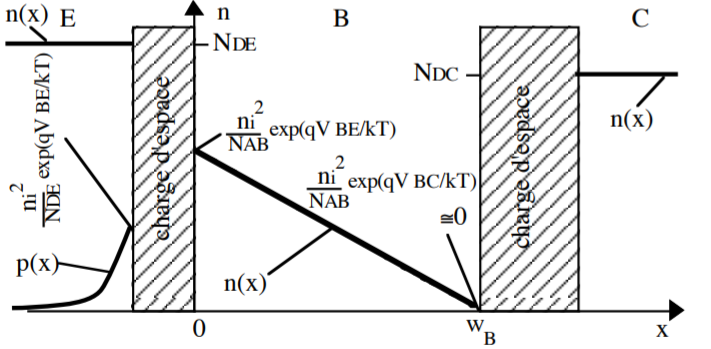
\includegraphics[width=0.6\textwidth]{LinEMmodel}
    \caption{Modèle des densités de porteurs linéarisés}
\end{figure}
Cette approximation revient à dire que les gradients sont les même dans la base, elle considère donc qu'il n'y a pas du tout de recombinaison dans la base.
\begin{figure}[H]
    \centering
    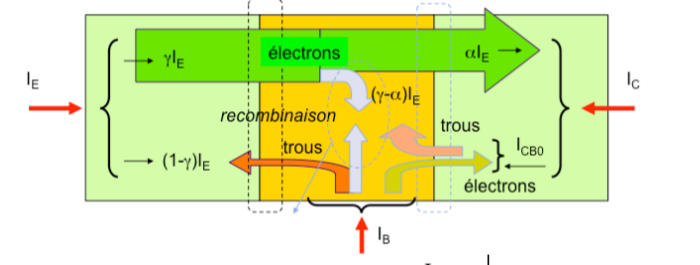
\includegraphics{Interpretation}
    \caption{Modèle complet du transfert de courant en régime actif des facteurs d'efficacité}
\end{figure}
\subsection{Caractéristiques }
Caractéristiques en fonction des configurations :
\begin{figure}[H]
    \centering
    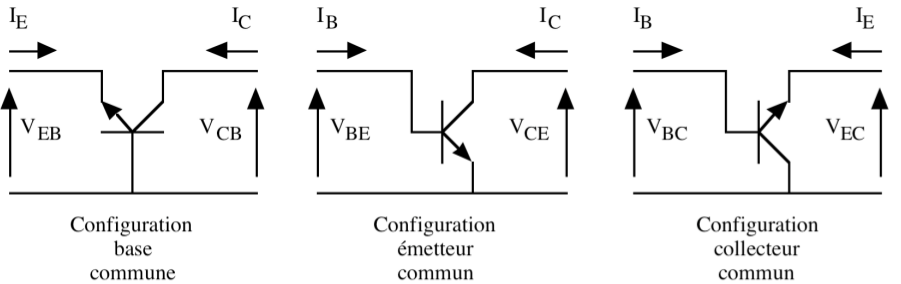
\includegraphics[width=0.9\textwidth]{Capture}
    \caption{Modes de fonctionnement et caractéristiques courant et tension}
\end{figure}
\subsection{Non-idéalitées}
\subsubsection{Effet Early}
L'effet early est du au changement de taille de la largeur de la base en fonction des zones de déplétion.
\begin{gather}
  { l } _ {   { CB } } ( 0 ) = \sqrt { \frac { 2 . \varepsilon _ {   { s } } } {   { q } } \cdot \frac { \phi _ {   { 0 } } \cdot   { N } _ {   { DC } } } {   { N } _ {   { AB } } ^ { 2 } } } \quad,\quad   { l } _ {   { CB } } \left(   { V } _ {   { CB } } \right) = \sqrt { \frac { 2 . \varepsilon _ {   { S } } } {   { q } } \cdot \frac { \left( \phi _ { 0 } +   { V } _ {   { CB } } \right) \cdot   { N } _ {   { DC } } } {   { N } _ {   { AB } } ^ { 2 } } }\\
    { w } _ {   { B } } \left(   { V } _ {   { CB } } \right) -   { w } _ {   { B } } ( 0 ) =   { l } _ {   { CB } } ( 0 ) \left( 1 - \sqrt { 1 + \frac {   { V } _ {   { CB } } } { \phi _ { 0 } } } \right)
\end{gather}
on injecte cette relation dans $\beta_F$ pour trouver la tension d'early en base commune
\begin{gather}
\beta _ { F } = \frac { J _ { n B } } { J _ { p E } } = \frac { \mu _ { n B } \cdot W _ { E } \cdot N _ { D E } } { \mu _ { p E } \cdot W _ { B } \cdot N _ { A B } }\\
  { I } _ {   { C } } = \beta _ {   { F } 0 }   { I } _ {   { B } } \left( 1 + \frac {   { V } _ {   { CE } } } {   { V } _ {   { EA } } } \right)
\end{gather}
Dans le cas de émetteur commun
\begin{gather}
{ I } _ { C } = - \alpha _ { F 0 } I _ { E } \left( 1 + \frac { V _ { C B } } { V _ { E A B } } \right)\\
  { V } _ {   { EAB } } = \left( \beta _ {   { F } 0 } + 1 \right) \cdot   { V } _ {   { EA } }
\end{gather}
On peut interpréter ça comme la pente de la fonction courant tension dans les cas base commune et émetteur commun.
\begin{figure}[H]
    \centering
    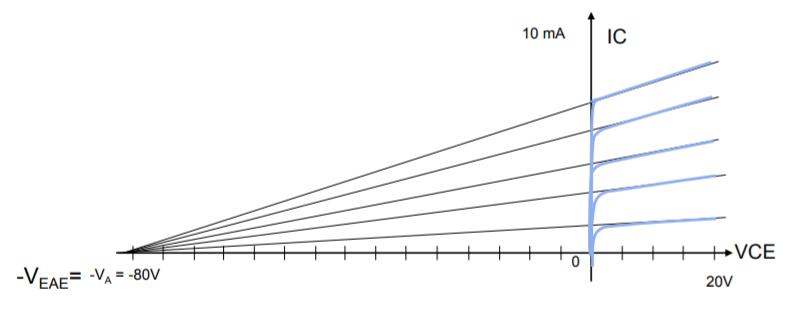
\includegraphics[width=0.6\textwidth]{penteVea}
    \caption{Interprétation de l'effet early}
\end{figure}
\begin{figure}[H]
    \centering
    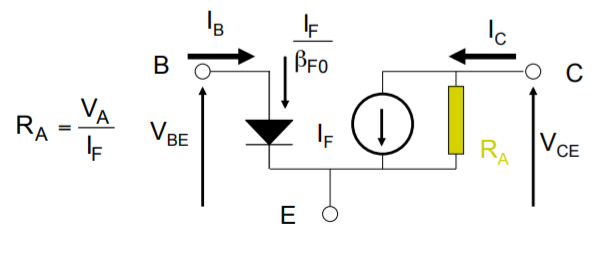
\includegraphics[width=0.6\textwidth]{modVea}
    \caption{Modèle de l'effet early}
\end{figure}
\subsubsection{Recombinaison dans la jonction base émetteur}
Comme vu dans la diode, il existe un courant de recombinaison dans la zone de déplétion
\begin{gather}
J _ { r , g } = J _ { s , r , g } \left( e ^ { q V / 2 k T } - 1 \right)
\end{gather}
valable pour les tension où le courant de saturation de génération recombinaison est supérieur.
\subsubsection{Effet Kirk}
$\beta_F$ dépend de la polarisation. À très faible injection le courant de recombinaison est le plus influent. À forte injection (courants élevés) il y a injection de minoritaires dans la base, on appelle ça l'effet Kirk.
\subsubsection{Résistance parasite}
Les résistances des fils font office de résistances parasites, le modèle devient alors
\begin{gather}
  { V } _ {   { BE } } = \left.   { V } _ {   { BE } } \right| _ { \text { a la jonction } } = \left.   { V } _ {   { BE } } \right| _ {   { aux } \text { bornes du transistor } } -   { I } _ {   { B } }   { R } _ {   { B } }
\end{gather}
Le courant augmentant exponentiellement, réduit la tension de manière exponentielle également en régime actif
\begin{equation}
  { I } _ {   { C } } =   { I } _ {   { TS } } \exp \left[ \frac {   { q } \left( \left.   { V } _ {   { BE } } \right| _ { \text { aux bornes du transistor } } -   { I } _ {   { B } }   { R } _ {   { B } } \right) } {   { kT } } \right]
\end{equation}
\subsubsection{Effet de la température}
Le courant de saturation dépend de la température. et suit une loi de la forme
\begin{gather}
I _ { F } ( T ) \equiv I _ { s } ( T ) e ^ { \frac { V _ { B E } } { q _ { T } } }\\
  { I } _ {   { s } } (   { T } ) \cong   { I } _ {   { s } } \left(   { T } _ { 0 } \right) \left( \frac {   { T } } {   { T } _ { 0 } } \right) ^ {   { mB } }   { e } ^ { - \frac {   { V } _ {   { g } } } { \phi _ {   { TO } } } \left( \frac {   { T } _ { 0 } } {   { T } } - 1 \right) }
\end{gather}
Ainsi, pour garder le courant constant, il faut appliquer un delta de tension
\begin{gather}
\delta   { V } _ {   { th } } = \frac { -   { V } _ {   { gb } } } {   { T } _ {   { o } } } \cdot \left(   { T } -   { T } _ {   { o } } \right)
\end{gather}
\subsubsection{$\beta_F$ en fonction de la température}
Par identification dans $\beta_F$ on trouve la dépendance à la température
\begin{equation}
\beta _ {   { F } } (   { T } ) = \beta _ {   { F } } \left(   { T } _ {   { o } } \right) \left( \frac {   { T } } {   { T } _ {   { o } } } \right) ^ { \left(   { m } _ {   { B } } -   { m } _ {   { E } } \right) } \exp \left[ \frac {   { E } _ {   { gB } } -   { E } _ {   { gE } } } {   { kT } _ {   { o } } } \left( \frac {   { T } _ {   { o } } } {   { T } } - 1 \right) \right]
\end{equation}
et le delta de courant au collecteur pour maintenir le courant à l'émetteur constant est donc
\begin{equation}
\delta   { I } _ {   { th } } (   { T } ) =   { I } _ {   { B } } \frac { \beta _ {   { F } } (   { T } ) - \beta _ {   { F } } \left(   { T } _ {   { o } } \right) } { \beta _ {   { F } } (   { T } ) }
\end{equation}
\subsection{Modèle dynamique}
De la même manière que pour la diode, on distinguera les différentes zones chargées dont la différence de potentiel fera varier la charge. On fait l'approximation quasi statique
\begin{gather}
I = \frac { d Q } { d t } = \frac { d } { d t } [ Q ( V ) ] = \frac { d Q } { d V } \frac { d V } { d t }
\end{gather}
Les charges des minoritaires dans la base
\begin{gather}
Q _ { F } = q A \int _ { 0 } ^ { w _ { B } } n ^ { \prime } ( x ) d x = \frac { 1 } { 2 } A q w _ { B } \frac { n _ { i } ^ { 2 } } { N _ { a B } } \left( \exp \left( \frac { q V _ { B E } } { k T } \right) - 1 \right)\\
  { Q } _ {   { F } } =   { Q } _ {   { F } 0 } \left( \exp \left( \frac {   { q }   { V } _ {   { BE } } } {   { kT } } \right) - 1 \right)\quad,\quad Q _ { F 0 } = \frac { 1 } { 2 } A q w _ { B } \frac { n _ { i } ^ { 2 } } { N _ { a B } }
\end{gather}
Sans le courant de recombinaison, on exprime le courant de collecteur,et en identifiant $Q_F$
\begin{gather}
  { I } _ {   { C } } = -   { A }   { J } _ {   { n } } = -   { A }   { q }   { D } _ {   { n }   { B } } \frac {   { d }   { n } ^ { \prime } } {   { dx } } = \frac {   { qAD } _ {   { nB } }   { n } _ {   { i } } ^ { 2 } \left( \exp \left( \frac {   { q }   { V } _ { BE } } {   { kT } } \right) - 1 \right) } {   { N } _ {   { aB } }   { w } _ {   { B } } }\\
   { I } _ {  { C } } = \frac { 2  { D } _ {  { nB } } } { w_B^2 }  { Q } _ {  { F } }
\end{gather}
On finit par trouver les realtaions, avec $\tau_F$ le temps de transit au travers de la base
\begin{gather}
 { I } _ {  { C } } = \frac {  { Q } _ {  { F } } } {  { T } _ {  { F } } } \quad,\quad \tau _ { F } = \frac { w _ { B } ^ { 2 } } { 2 D _ { n B } }\\
 { I } _ {  { C } } =  { I } _ {  { TS } } \left[ \exp \left( \frac{ { qV } _ {  { BE } }}{ { kT } }\right) - 1 \right] \quad,\quad  { I } _ {  { TS } } = \frac {  { Q } _ {  { F } 0 } } { \tau _ {  { F } } }
\end{gather}
De manière analogue on reliera les autres courant aux charges déplacées $I_B = -(I_{pE}-I_{rB})$
\begin{gather}
 { I } _ {  { pE } } =  { A }  { J } _ {  { pE } } = - \frac {  { q }  { A }  { D } _ {  { pE } }  { p } _ {  { OE } } } {  { L } _ {  { pE } } } \left[ \exp \left( \frac {  { qV } _ {  { BE } } } {  { kT } } \right) - 1 \right] = - \frac { 2  { D } _ {  { pE } }  { p } _ {  { oE } } } {  { L } _ {  { pE } }  { w } _ {  { B } }  { n } _ {  { oB } } }  { Q } _ {  { F } }\\
 { I } _ {  { rB } } =  { A } \left(  { J } _ {  { nE } } -  { J } _ {  { nC } } \right) = - \frac {  { qA } } { \tau _ {  { n } } } \int _ { 0 } ^ {  { w } _ {  { b } } } \left(  { n } - \frac {  { n } _ {  { i } } ^ { 2 } } {  { N } _ {  { aB } } } \right)  { d }  { x } = - \frac {  { Aq } } { \tau _ {  { n } } } \frac {  { w } _ {  { B } } } { 2 }  { n } ^ { \prime } ( 0 ) = - \frac {  { Q } _ {  { F } } } { \tau _ {  { n } } }
\\
 { I } _ {  { B } } = -  { I } _ {  { pE } } -  { I } _ {  { rB } } = \left( \frac { 2  { D } _ {  { pE }  { p } _ {  { oE } } } } {  { w } _ {  { B } }  { L } _ {  { pE } }  { n } _ {  { oB } } } + \frac { 1 } { \tau _ {  { n } } } \right)  { Q } _ {  { F } } = \frac {  { Q } _ {  { F } } } { \tau _ {  { BF } } } \quad,\quad \tau _ {  { BF } } = \frac { 1 } { \frac { 2  { D } _ {  { pE } }  { p } _ {  { oE } } } {  { w } _ {  { B } }  { L } _ {  { pE } }  { n } _ {  { oB } } } + \frac { 1 } { \tau _ {  { n } } } }
\end{gather}
Il s'avère que le courant de recombinaison est négligeable dans le cas d'une base courte, ce qui se voit immédiatement au temps de transit $\tau _ { F } \ll \tau _ { n }$, à savoir
\begin{gather}
 { w } _ {  { B } } ^ { 2 } \ll 2  { D } _ {  { nB } } \tau _ {  { n } } = 2  { L } _ {  { nB } } ^ { 2 }
\end{gather}
En résumé, les équations de charges respectivement $D$ déplétion et $F,R$ diffusion, en fonction de la tension sont sont
\begin{gather}
\phi _ { 0 E } = \phi _ { \top } \ln \left( \frac { N _ { A B }  N _ { D E } } { n _ { i } ^ { 2 } } \right) \quad,\quad \phi _ { 0 C } = \phi _ { T } \ln \left( \frac { N _ { A B } N _ { D C } } { n _ { i } ^ { 2 } } \right)\\
 { Q } _ {  { DE } } =  { Q } _ {  { DE } 0 } \sqrt { \frac { \phi _ { 0  { E } } -  { V } _ {  { BE } } } { \phi _ { 0  { E } } } } \quad,\quad Q _ { D C } = Q _ { D C 0 } \sqrt { \frac { \phi _ { 0 C } - V _ { B C } } { \phi _ { 0 C } } }\\
 Q _ { F } = \tau _ { T } I _ { s } \left[ e ^ { \frac { V _ { B E } } { \phi _ { T } } } - 1 \right] \quad,\quad  { Q } _ {  { R } } = \tau _ {  { T } } I_ {  { s } } \left[  { e } ^ { \frac {  { V } _ {  { BC } } } { \phi _ {  { T } } } } - 1 \right]
\end{gather}
Ce qui nous donne le modèle suivant
\begin{figure}[H]
    \centering
    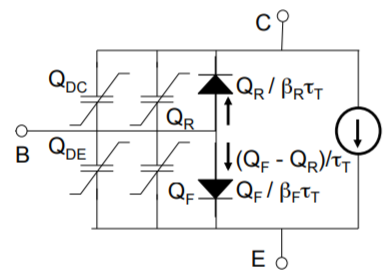
\includegraphics[width=0.6\textwidth]{CappaBJT}
    \caption{Modèle dynamique complet du BJT}
\end{figure}
\subsection{Modèle petit signal}
Comme d'habitude, on dérive le modèle petit signal depuis le développement en série autour du point de polarisation. On traite ici le régime actif tel que donné par le schéma 
\begin{figure}[H]
    \centering
    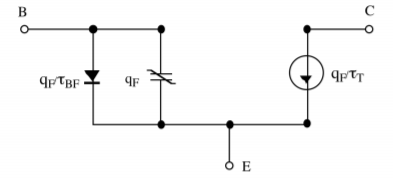
\includegraphics[width=0.6\textwidth]{PSBJT}
    \caption{Modèle dynamique complet du BJT}
\end{figure}
\begin{gather}
 { V } _ {  { BE } } (  { t } ) =  { V } _ {  { BEo } } +  { v } _ {  { BE } } (  { t } ) \quad,\quad I_C(t) = { I } _ {  { Co } } +  { i } _ {  { C } }(t)\\
 { I } _ {  { C } } = \frac {  { Q } _ {  { F } } } { \tau _ {  { T } } }\\
  I_C(V_{V_{BEo}})+v_{BE}\frac{dI_C}{dV_{BE}}\vert_{V_{BEo}}= { I } _ {  { Co } } +  { i } _ {  { C } } = \frac{Q_{F0}}{\tau_T}\left[ e ^ { \frac { V _ { B E } } { \phi T } } - 1 \right]+v_{BE}\frac { q  } { k T } \frac { Q _ { F 0 } } { \tau _ { T } } \exp \left(\frac{ V _ { B E o } }{\phi _ { T } ^ { \prime }} \right)
\end{gather}
On identifie respectivement la composante DC et AC
\begin{gather}
 { I } _ {  { Co } } = \frac {  { Q } _ {  { F } 0 } } { \tau _ {  { T } } } \left[ \exp \left(  { V } _ {  { BE }  { o } } / \phi _ {  { T } } \right) - 1 \right] \quad,\quad   { i } _ {   { C } } =   { g } _ {   { m } }   { v } _ {   { BE } } \quad,\quad  { g } _ {  { m } } = \frac {  { q } } {  { k }  { T } }  { I } _ {  { Co } }
\end{gather}
Idem pour $I_B$
\begin{gather}
 { I } _ {  { B } } = \frac {  { Q } _ {  { F } } } { \tau _ {  { BF } } } + \frac {  { d }  { Q } _ {  { F } } } {  { dt } }\\
 { I } _ {  { Bo } } +  { i } _ {  { B } } = \frac { Q _ { F 0 } } { \tau _ { T } } \left[ \exp \left( V _ { B E o } / \phi _ { T } \right) - 1 \right]+\frac { q } { k T }  Q _ { F 0 } \exp \left( \frac { V _ { B E o } } { \phi _ { T } ^ { \prime } } \right)\left( \frac { v _ { B E } } { \tau _ { B F } } + \frac { d v _ { B E } } { d t } \right)\\
 { I } _ {  { Bo } } = \frac {  { Q } _ {  { F } 0 } } { \tau _ {  { BF } } } \left[ \exp \left(  { V } _ {  { BE }  { d } } / \phi _ {  { T } } ^ { \prime } \right) - 1 \right] \quad,\quad  { i } _ {  { B } } = \frac { { v } _ {  { BE } } } {  { r } _ { \pi } } +  { C } _ {  { F } } \frac { { d }  { v } _ {  { BE } } } {  { dt } }\\
 \frac {  { v } _ {  { BE } } } { \tau _ {  { BF } } } = r _ { \pi } = \frac { \tau _ { B F } } { \tau _ { T } } \frac { 1 } { g _ { m } } \quad,\quad \frac {  { d }  { v } _ {  { BE } } } {  { dt } } =  { C } _ {  { F } } =  { g } _ {  { m } } \tau _ {  { T } }
\end{gather}
Les capacités des zones de transitions sont données par 
\begin{gather}
C _ { E } = \frac { d q _ { E } } { d V _ { B E } }\quad,\quad  { C } _ {  { C } } = \frac {  { d } q _ {  { C } } } {  { d }  { V } _ {  { BC } } }
\end{gather}
Ce qui nous donne le modèle en $\pi$ hybride
\begin{figure}[H]
    \centering
    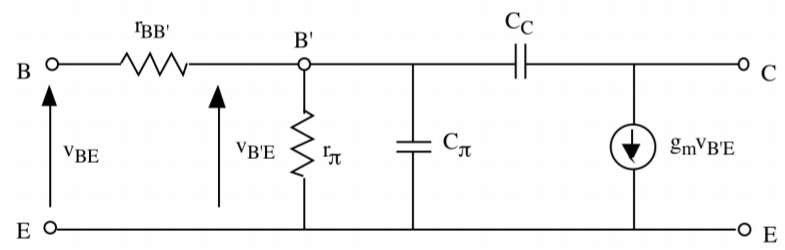
\includegraphics[width=0.6\textwidth]{PImodel}
    \caption{Modèle $\pi$ hybride complet du BJT}
\end{figure}
\section{MOSFET}
Le transistor MOS à effet de champ est composé d'une base dopé P (resp N) et de deux accès dopé N (resp P) ainsi que d'une grille séparé de la base par un isolant. La présence d'un champ dans la grille crée un canal de minoritaires (appelé canal d'inversion) dans le substrat reliant ainsi les deux accès. Celui-ci fonctionne comme un interrupteur. Le transistor MOSFET est parfaitement symétrique.
\begin{figure}[H]
    \centering
    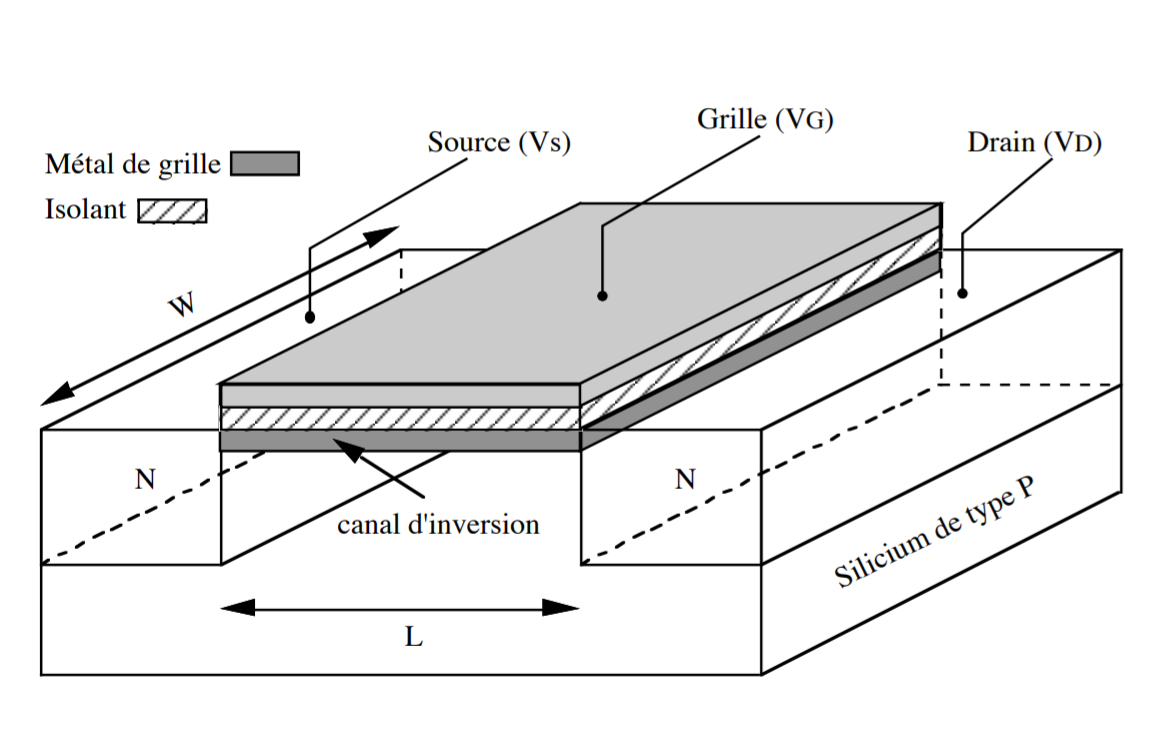
\includegraphics[width=0.6\textwidth]{MOSFET}
    \caption{Modèle 3D d'un MOSFET}
\end{figure}
Le canal est en forme de losange, voir de triangle selon la tension appliqué. En effet, la tension de source et de drain affecte la densité d'électrons de leur coté du MOS. à tension de source et drain égale, le canal est rectangulaire. Lorsque le canal ne relie pas les deux accès, on dit qu'il ya pinch-off et le courant est limité et le transistor en état saturé.
\subsection{Le canal de minoritaires}
Soit le canal dans un substrat tel que 
\begin{figure}[H]
    \centering
    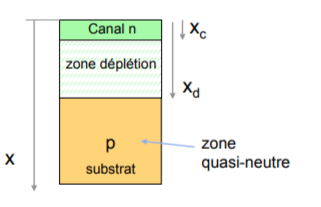
\includegraphics[width=0.5\textwidth]{canal}
    \caption{Canal et zone de déplétion d'un MOS}
\end{figure}
Les bandes d'énergie se rejoignent au niveau de Fermi au travers de l'isolant. Le matériau de la grille étant un métal, celui-ci n'a pas le même band gap. La présence d'une tension dans la grille fait varier le niveau de Fermi dans le métal. Pour rester à l'équilibre il y a courbure de bande dans le substrat. Il apparaît alors les trois cas suivant en fonction de la position du niveau de Fermi dans la bande du substrat.
\begin{figure}[H]
    \centering
    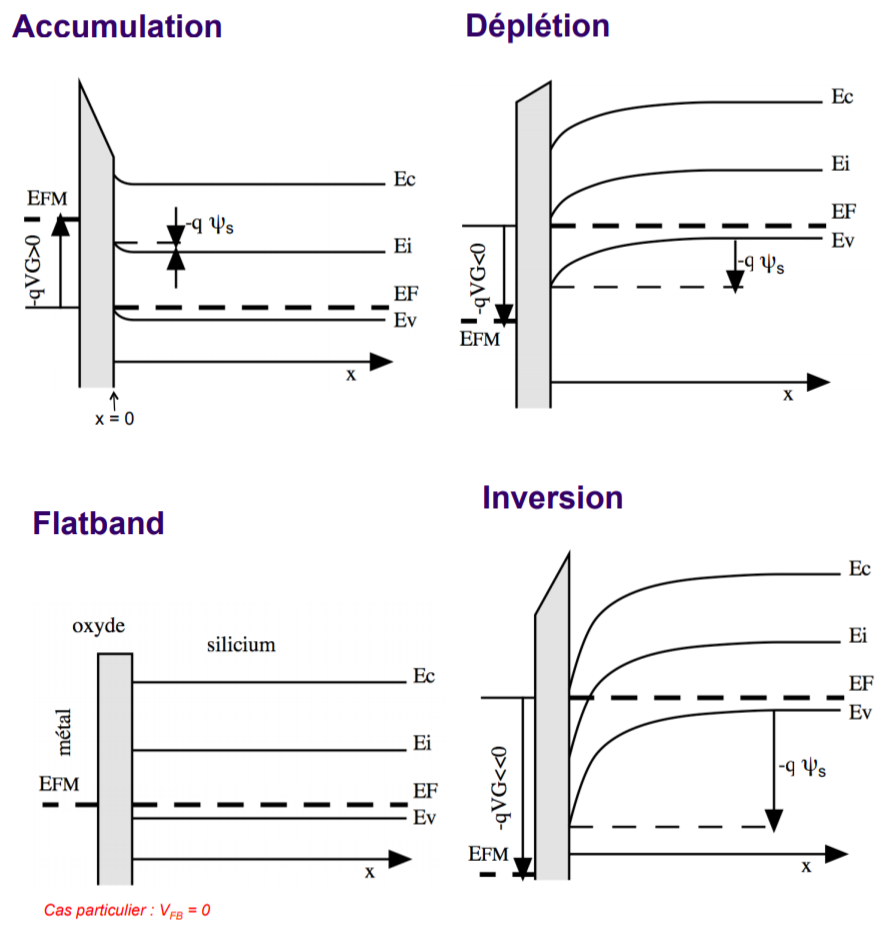
\includegraphics[width=0.7\textwidth]{MOSBands}
    \caption{Canal et zone de déplétion d'un MOS}
\end{figure}

\subsection{Modèle linéarisé}
Soit la tension seuil $V_{TH}$, la charge du canal et la capacité sont
\begin{gather}
 { Q } = -  { WL }  { C } _ {  { ox } } \left(  { V } _ {  { G } } -  { V } _ {  { TH } } \right) \quad,\quad  { C } _ {  { ox } } = \varepsilon _ {  { ox } } /  { t } _ {  { ox } }
\end{gather}
Le courant
\begin{gather}
 { I } _ {  { D } } = -  { Q } / \tau
\end{gather}
La tension $V_{DS}$ étant pratiquement constante, la vitesse de dérive est donnée par
\begin{gather}
 { v } _ {  { dn } } = \mu _ {  { n } }  { V } _ {  { DS } } /  { L }
\end{gather}
Le temps de transit $\tau$
\begin{gather}
\tau = \frac{L}{ v _ { n }} = \frac{L ^ { 2 }}{\mu _ { n } V _ { D S }}
\end{gather}
donc 
\begin{gather}
I _ { D } = \frac{- Q }{ \tau} = -\frac{- W L C _ { o x } \left( V _ { G } - V _ { T H } \right)}{\frac { L ^ { 2 } } { \mu _ { n } V _ { D S } }} = \frac{W}{L}\mu _ {  { n } }  { C } _ {  { ox } } \left(  { V } _ {  { G } } -  { V } _ {  { TH } } \right)  { V } _ {  { DS } }
\end{gather}
On Peut modéliser la variation de courant en fonction de la tension comme une résistance non-linéaire
\begin{gather}
 { I } _ {  { D } } = \frac{ { V } _ {  { DS } } }{  { R } _ {  { CH } }} \quad,\quad R_{CH} = \frac{L}{ { W } \mu _ {  { n } }  { C } _ {  { ox } } \left(  { V } _ {  { G } } -  { V } _ {  { TH } } \right)}
\end{gather}
On a donc un modèle valable à faibles tensions $V_{DS}$
\begin{figure}[H]
    \centering
    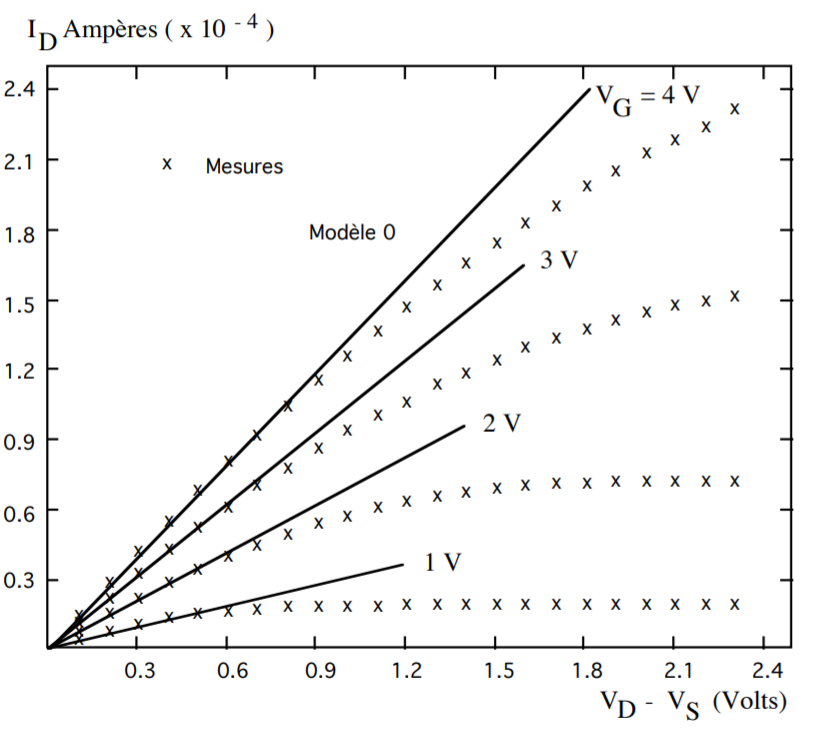
\includegraphics[width=0.6\textwidth]{LINMOS}
    \caption{Modèle linéarisé du MOS, mesures VS modèle}
\end{figure}


\subsection{Analyse des charges}
\subsubsection{Déplétion}
Soit les charges en présence en fonction de la tension dans un substrat de type P
\begin{gather}
 { p } (  { x } ) =  { N } _ {  { A } } \cdot  { e } ^ { \frac { - \psi (  { x } ) } {  { \phi } _ {  { T } } } }\quad,\quad n ( x ) = \frac { n _ { i } ^ { 2 } } { N _ { A } } \cdot e ^ { \frac { \psi ( x ) } { \phi _ { T } } }=  { N } _ {  { A } } \cdot  { e } ^ { \frac { \psi (  { x } ) - 2 . \phi  { F } } {  { \phi } _ {  { T } } } }
\end{gather}
Dans le cas déplétion, les charges sont constantes et égales au dopage (cf jonciton PN)
\begin{gather}
\rho ( x ) = q \left[ p ( x ) - n ( x ) - N _ { A } \right]\cong - q N _ { A }\\
E ( x ) = - \frac { d \psi } { d x } = - \frac { q \cdot N _ { A } } { \varepsilon _ { s } } \cdot \left( x - x _ { d } \right)\quad,\quad E \left( x _ { d } \right) = 0\\
\frac {  { d } ^ { 2 } \psi (  { x } ) } {  { dx } ^ { 2 } } = - \frac { \rho (  { x } ) } {  { e } _ {  { s } } }\quad,\quad \psi ( 0 ) = \psi _ {  { S } } = \frac {  { q } \cdot  { N } _ {  { A } } } { 2 \cdot \varepsilon _ {  { S } } } \cdot  { x } _ {  { d } } ^ { 2 } \quad,\quad \operatorname { avec } \quad \psi \left(  { x } _ {  { d } } \right) = 0
\end{gather}
On trouve finalement la longueur de déplétion et la charge
\begin{gather}
 { x } _ {  { d } } = \sqrt { \frac { 2 . \varepsilon _ {  { s } } } {  { q } \cdot  { N } _ {  { A } } } \cdot \psi _ {  { s } } }\\
Q _ { D } ^ { \prime } = - q \cdot N _ { A } \cdot x _ { d } = - \sqrt { 2 \varepsilon _ { s } \cdot q _ { A } \cdot N _ { A } \cdot \psi_S }
\end{gather}
On définit la taille de la zone de déplétion maximale est définit comme la longueur à laquelle la tension permet à l'énergie de Fermi de rejoindre la bande de conduction. On peut approximer ça également par la condition que la densité d'électrons dans le canal doit être égal au nombre de trous dans le substrat, ce qui impose à la tension $\psi _ { s } ( y ) \geq 2 \phi _ { F }$
\begin{gather}
\psi _ {  { s } } (  { y } ) = 2 \phi _ {  { F } } +  { V } (  { y } )\\
 { x } _ {  { d } ,  { max } } = \sqrt { \frac { 2 \varepsilon _ {  { s } } } {  { q }  { N } _ {  { A } } } \left[ 2 \phi _ {  { F } } +  { V } (  { y } ) \right] }\\
 { Q } _ {  { D } } (  { y } ) = -  { q }  { N } _ {  { A } }  { x } _ {  { d } ,  { max } } = - \sqrt { 2 \varepsilon _ {  { s } }  { q }  { N } _ {  { A } } \left[ 2 \phi _ {  { F } } +  { V } (  { y } ) \right] }
\end{gather}
On remarque deux choses :
\begin{itemize}
    \item La tension dépend de la position en $y$, pour prendre en compte l'influence de $V_{DS}$
    \item Lorsque la tension de grille est égale à la tension seuil, le canal d'inversion est à son maximum et ne varie que très peu ($\sqrt{V(y)}$)
\end{itemize}
\subsubsection{Inversion}
L'inversion est atteinte lorsque la concentration en électron sous tension est égale à la concentration en trous à l'équilibre. D'abord inspectons le bilan de charge.
\begin{figure}
    \centering
    \includegraphics{Charges.PNG}
    \caption{Analyse spatiale des charges et du potentiel}
\end{figure}
qui se traduit par le bilan de charge, de potentiel et Gauss
\begin{gather}
Q _ { G } ^ { \prime } = - Q _ { s c } ^ { \prime } - Q _ { o x } ^ { \prime } = - \left( Q _ { c } ^ { \prime } + Q _ { D } ^ { \prime } \right) - Q _ { o x }\\
 { V } _ {  { GB } } - \phi _ {  { ms } } = \psi _ {  { s } } +  { V } _ {  { ox } }\\
 - \varepsilon _ {  { ox } } \cdot  { E } _ {  { x } } =  { Q } _ {  { sc } } ^ { \prime } +  { Q } _ {  { ox } } \quad,\quad  { E } _ {  { x } } =  { V } _ {  { ox } } /  { e } _ {  { ox } }\\
  { Q } _ {  { sc } } ^ { \prime } = -  { C } _ {  { ox } } \cdot \left[  { V } _ {  { GB } } - \psi _ {  { S } } -  { V } _ {  { FB } } \right] =  { Q } _ {  { C } } ^ { \prime } +  { Q } _ {  { D } } ^ { \prime }
\end{gather}
à la tension seuil on a 
\begin{gather}
 { V } _ {  { GB } } =  { V } _ {  { F }  { B } } + \psi _ {  { s } } - \frac {  { Q } _ {  { C } } ^ { \prime } +  { Q } _ {  { D } } ^ { \prime } } {  { C } _ {  { Ox } } ^ { \prime } }\\
Q _ { c } = 0 \quad\text {et}\quad \psi _ { s } = 2 . \phi _ {  { F } }\\
 { V } _ {  { TH } } =  { V } _ {  { FB } } + 2 . \phi _ {  { F } } -  { Q } _ {  { D } } ^ { \prime } /  { C } _ {  { ox } }\\
 { V } _ {  { TH } } =  { V } _ {  { FB } } + 2 . \phi _ {  { F } } + \frac{\sqrt { 2q \varepsilon _ {  { S } } N _ {  { A } } }}{ { C } _ {  { ox } } ^ { \prime }}\sqrt { 2 . \phi _ {  { F } } }= V _ { TH 0 }
\end{gather}
La tension étant aussi influencé par la tension à la source, on écrit $V_{GB} = 2 \phi _ {  { F } } +  { V }_s$
\begin{gather}
 { V } _ {  { TH } } =  { V } _ {  { FB } } + 2 \phi _ {  { F } } +  { V } _ {  { s } } + \frac { 1 } {  { C } _ {  { ox } } } \sqrt { 2 \varepsilon _ { s }  { q }  { N } _ {  { A } } \left[ 2 \phi _ {  { F } } +  { V } _ {  { s } } \right. } ]\\
 { V } _ {  { THo } } =  { V } _ {  { FB } } + 2 \phi _ {  { F } } + \frac { 1 } {  { C } _ {  { ox } } } \sqrt { 2 \varepsilon _ {  { s } }  { q }  { N } _ {  { A } } \left( 2 \phi _ {  { F } } \right) } \quad,\quad V_s = 0\\
 V _ { T H } -V_s = V _ { F B } + 2 \phi _ { F }  + \frac { 1 } { C _ { o x } } \sqrt { 2 \varepsilon _ { s } q N _ { A } \left[ 2 \phi _ { F } + V _ { s } \right. } ]\\
 { V } _ {  { TH } } -  { V } _ {  { s } } =  { V } _ {  { THo } } + \frac { 1 } {  { C } _ {  { ox } } } \left[ \sqrt { 2 \varepsilon _ {  { s } }  { q }  { N } _ {  { A } } \left[ 2 \phi _ {  { F } } +  { V } _ {  { s } } \right] } - \sqrt { 2 \varepsilon _ {  { s } }  { q }  { N } _ {  { A } } \left( 2 \phi _ {  { F } } \right) } \right]
\end{gather}
On observe que la tension combiné $V_{GS}$ provoque un glissement de la fonction $I_D$ - $V_{TH}$.


\subsection{Effet de substrat}
Appliquer un potentiel à la source (avec la base comme référence) fait changer le potentiel seuil à appliquer pour obtenir l'effet d'inversion et changeant la tension de seuil.
\begin{gather}
 { V } _ {  { TH } } =  { V } _ {  { FB } } + 2 . \phi _ {  { F } } +  { V } _ {  { CB } } + \frac { \sqrt { 2q \varepsilon _ {  { s } }  { N } _ {  { A } } } } {  { C } _ {  { ox } } ^ { \prime } } \cdot \sqrt { 2 . \phi _ {  { F } } +  { V } _ {  { CB } } }\\
V_{TH} =  { V } _ {  { T } 0 } + \lambda \cdot  { V } _ {  { SB } }\quad,\quad \lambda = 1 + \frac { \sqrt { 2 \varepsilon _ {  { s } }  { q }  { N } _ {  { A } } } } { 2  { C } _ {  { ox } } \sqrt { 2 \Phi _ {  { F } } } }
\end{gather}
Cela est du à la forme triangulaire du canal, l'inversion n'est plus atteinte tout le long du canal. La relation tension-courant se retrouve shifté de racine du potentiel $V_S$ 
\begin{equation}
 { V } _ {  { TH } } -  { V } _ {  { S } } =  { V } _ {  { THo } } + \frac { 1 } {  { C } _ {  { ox } } } \left[ \sqrt { 2 \varepsilon _ {  { s } }  { q }  { N } _ {  { A } } \left[ 2 \phi _ {  { F } } +  { V } _ {  { s } } \right] } - \sqrt { 2 \varepsilon _ {  { s } }  { q }  { N } _ {  { A } } \left( 2 \phi _ {  { F } } \right) } \right]
\end{equation}
\subsection{Courant dans le MOS}
Le courant est calculé sur base des charges présentes
\begin{gather}
 { dV } =  { I } _ {  { D } }  { dR } = - \frac {  { I } _ {  { D } }  { d }  { y } } {  { W } \mu _ {  { n } }  { Q } _ {  { N } } (  { y } ) }
\end{gather}
Le courant étant constant on peut écrire en fonction de la charge, avec $V_T(y)$ la tension seuil à la position $y$
\begin{gather}
 { I } _ {  { D } } \int _ { 0 } ^ {  { L } }  { d }  { y } = -  { W } \mu _ {  { n } } \int _ {  { V } _ {  { S } } } ^ {  { V } _ {  { D } } }  { Q } _ {  { N } }  { dV }= - \frac {  { W } } {  { L } } \mu _ {  { n } } \int _ {  { V } _ {  { s } } } ^ {  { V } _ {  { D } } }  { Q } _ {  { N } }  { dV }\\
  { Q } _ {  { N } } = -  { C } _ {  { ox } } \left[  { V } _ {  { G } } -  { V } _ {  { T } } (  { y } ) \right]\\
  { I } _ {  { D } } = \frac {  { W } } {  { L } } \mu _ {  { n } }  { C } _ {  { ox } } \int _ {  { V } _ {  { s } } } ^ {  { V } _ {  { D } } } \left[  { V } _ {  { G } } -  { V } _ {  { T } } (  { y } ) \right]  { d }  { V }\\
   { V } _ {  { T } } (  { y } ) =  { V } _ {  { FB } } + 2 \phi _ {  { F } } +  { V } (  { y } ) + \frac { 1 } {  { C } _ {  { ox } } } \sqrt { 2 \varepsilon _ {  { s } }  { q }  { N } _ {  { A } } \left[ 2 \phi _ {  { F } } +  { V } (  { y } ) \right] }
\end{gather}
Après linéarisation du terme $V_T(y)$ pour obtenir une relation linéraire, on trouve les expressions
\begin{gather}
 { V } _ {  { T } } (  { y } ) =  { V } _ {  { THo } } + \lambda  { V } (  { y } ) \quad,\quad \lambda = 1 + \frac { \sqrt { 2 \varepsilon _ {  { s } } q N _ { A } } } { 2 C _ { \text { ox } } \sqrt { 2 \phi _ {  { F } } } }
\end{gather}
ce qui permet de faire une simple intégration sur le courant pour trouver la charge
\begin{figure}[H]
    \centering
    \includegraphics[width=0.6\textwidth]{IntegralMOS}
    \caption{Intégrale sur la tension pour trouver la charge $Q_N$}
\end{figure}
Les équations en utilisant la tension seuil linéarisé sont
\begin{gather}
 { I } _ {  { D } } = \frac {  { W } } {  { L } } \mu _ {  { n } }  { C } _ {  { ox } } \int _ {  { V } _ {  { s } } } ^ {  { V } _ {  { D } } } \left(  { V } _ {  { G } } -  { V } _ {  { THo } } - \lambda  { V } \right)  { dV } \\
 { I } _ {  { D } } = \frac {  { W } } {  { L } } \mu _ {  { n } }  { C } _ {  { ox } } \left[ \left(  { V } _ {  { G } } -  { V } _ {  { THo } } \right) \left(  { V } _ {  { D } } -  { V } _ {  { S } } \right) - \frac { \lambda } { 2 } \left(  { V } _ {  { D } } ^ { 2 } -  { V } _ {  { S } } ^ { 2 } \right) \right]
\end{gather}
On réutilise la relation $ { V } _ {  { TH } } =  { V } _ {  { THo } } + \lambda  { V } _ {  { s } }$
\begin{gather}
 { I } _ {  { D } } = \frac {  { W } } {  { L } } \mu _ {  { n } }  { C } _ {  { ox } } \left[\left(  { V } _ {  { G } } -  { V } _ {  { TH } } \right)  { V } _ {  { DS } } - \frac { \lambda } { 2 }  { V } _ {  { DS } } ^ { 2 } \right]
\end{gather}
On cherche la tension de drain pour la saturation en cherchant le maximum de la relation courant tension ($V_S = 0 \Rightarrow V_{DS} = V_D$)
\begin{gather}
\frac{dI_D}{dV_D} = 0 = \frac {  { W } } {  { L } } \mu _ {  { n } }  { C } _ {  { ox } } \left[ \left(  { V } _ {  { G } } -  { V } _ {  { TH } } \right) - \lambda { V } _ {  { D } } \right]\\
 { V } _ {  { D } ,  { sat } } = \frac { 1 } { \lambda } \left(  { V } _ {  { G } } -  { V } _ {  { THo } } \right) = \frac { 1 } { \lambda } \left(  { V } _ {  { G } } -  { V } _ {  { TH } } + \lambda  { V } _ {  { s } } \right) = \frac { 1 } { \lambda } \left(  { V } _ {  { G } } -  { V } _ {  { TH } } \right) +  { V } _ {  { s } }\\
  { V } _ {  { D,Sat } } =  { V } _ {  { D, }  { sat } } -  { V } _ {  { S } } = \frac { 1 } { \lambda } \left(  { V } _ {  { G } } -  { V } _ {  { TH } } \right)
\end{gather}
Soit le courant de saturation
\begin{gather}
 { I } _ {  { D }  { sat } } = \frac {  { W } } {  { L } } \mu _ {  { n } }  { C } _ {  { ox } } \frac { \left(  { V } _ {  { G } } -  { V } _ {  { TH } } \right) ^ { 2 } } { 2 \lambda }
\end{gather}
\subsection{Analyse}
\subsubsection{Paramètres et technologies}
Les différents paramètres influençables sont :
\begin{itemize}
    \item $V_{T0}$ choisi au travers du dopage
    \item $\mu_n$ la mobilité du au dopage
    \item $C_{ox}$ dépend de l'épaisseur de l'oxyde
    \item $\lambda$ dépend des dimension, en grande partie de la longueur du canal
    \item $W,L$ les dimensions reliant la densité de courant et la longueur du canal
\end{itemize}
\subsubsection{Effets du deuxième ordre}
\begin{itemize}
    \item Effet early :
    \begin{equation}
     { l } _ {  { D } } = \left[ 1 + \frac {  { V } _ {  { D } } -  { V } _ {  { DSat } } } {  { V } _ {  { A } } } \right] \left[ \frac { 1 } { 2 } \mu  { C } _ {  { ox } } \frac {  { W } } {  { L } } \frac { \left(  { V } _ {  { G } } -  { V } _ {  { TS } } \right) ^ { 2 } } { \lambda } \right]
    \end{equation}
    \item Courant de fuite
    \item À très haute tension : correction de la mobilité
    \begin{equation}
    \mu _ {  { n } } ^ { \prime } = \frac { \mu _ {  { n } } } { 1 + \theta \left(  { V } _ {  { G } } -  { V } _ {  { TS } } \right) }
    \end{equation}
    \item Pente de saturation :  notre modèle considère le courant à saturation constant, mais celui-ci évolue encore linéairement avec $V_{DS}$
\end{itemize}
\subsubsection{Effet de la modulation de la longueur de pinch off}
Soit notre modèle
\begin{gather}
 { I } _ {  { D } } \left(  { V } _ {  { D } } >  { V } _ {  { D } ,  { sat } } \right) = - \frac {  { W } } {  { L } - \Delta  { L } } \mu _ {  { eff } } \int _ {  { V } _ {  { S } } } ^ {  { V } _ {  { D } ,  { sat } } }  { Q } _ {  { N } }  { d }  { V }\\
  { I } _ {  { D } } \left(  { V } _ {  { D } } >  { V } _ {  { D } ,  { sat } } \right) = \frac {  { L } } {  { L } - \Delta  { L } }  { I } _ {  { D } ,  { sat } }\\
  \frac { I _ { D } \left( V _ { D } > V _ { D , s a t } \right) } { I _ { D , s a t } } = \frac { V _ { D S } + V _ { E } } { V _ { D , s a t } + V _ { E } }
\end{gather}
La longueur du canal total influence directement la répartition de la tension le long du transistor 
\subsubsection{Sous seuil}
L'augmentation du courant avec la tension en dessous de la tension seuil est exponentielle
\begin{gather}
I_D = I_010^{\frac{V_G-V_{TH}}{S}}\left(1-e^\frac{-V_{DS}}{\phi_T}\right)
\end{gather}
\subsubsection{Effet de la température}
La température est la source de courant de fuite, car la création de porteurs par génération dans le substrat permet à un courant de diffusion de circuler. 
\subsection{Comportement dynamique résistif}
En repartant du modèle complet
\begin{gather}
 { I } _ {  { D } } = \left[ 1 + \frac {  { V } _ {  { D } } -  { V } _ {  { DSat } } } {  { V } _ {  { A } } } \right] \left[ \frac { 1 } { 2 } \mu  { C } _ {  { ox } } \frac {  { W } } {  { L } } \frac { \left(  { V } _ {  { G } } -  { V } _ {  { TS } } \right) ^ { 2 } } { \lambda } \right]\\
  { V } _ {  { G } } =  { V } _ {  { GO } } +  { v } _ {  { G } } \quad\text { et }\quad  { V } _ {  { D } } =  { V } _ {  { DO } } +  { v } _ {  { D } }
\end{gather}
Le développement en série s'écrit
\begin{gather}
 { I } _ {  { D } } =  { I } _ {  { D }  { O } }\left( V _ { G 0 } , V _ { D 0 } \right)+\frac { \partial  { I_D } } { \partial  { V } _ {  { G } } }v_G+\frac { \partial I _ { D } } { \partial V _ { D } } v _ { D } \dots\\
  { g } _ {  { m } } = \frac { \partial  I_{ D } } { \partial  { V } _ {  { G } } } = 2 \cdot \frac {  I_{ Do } } {  { V } _ {  { G } } -  { V } _ {  { TS } } } \quad,\quad  { g } _ {  { d } } = \frac { \partial  I_{ D } } { \partial  { V } _ {  { D } } } = \frac { I_ { D } } {  { V } _ {  { A } } } 
\end{gather}
sont la transconductance et la conductance de sortie respectivement
\subsection{Comportement dynamique capacitif}
Il existe une capacité entre chaque accès
\begin{figure}[H]
    \centering
    \includegraphics[width=0.6\textwidth]{CappaMOS}
    \caption{Cappacités parasites du MOSFET}
\end{figure}
À forte inversion on considère les capacités d'overlap (capacités de recouvrement entre la grille et un accès séparé par l'oxyde) et les capacités de jonction PN bloqués, donc entre S-B et D-B.\\
Dans ce cas, si $V_{DS} = 0$
\begin{gather}
 { V } _ {  { DS } } = 0 :  { Q } _ {  { G } } \rightarrow  { C } _ {  { GS } } =  { C } _ {  { GD } } =  { W } \cdot  { L } \cdot  \frac{{ C } _ {  { ox } } }{2}
\end{gather}
À tension $V_{DS} \neq 0$, le modèle est
\begin{equation}
 { Q } _ {  { GS } } \rightarrow  { C } _ {  { GS } } = { W } .  { L } \frac{2 { C } _ {  { ox } }}{3} \quad,\quad { Q } _ {  { GD } } = 0 \rightarrow  { C } _ {  { GD } } = 0 !
\end{equation}
Le modèle complet est donc
\begin{figure}[H]
    \centering
    \includegraphics[width=0.6\textwidth]{PSModelMOS}
    \caption{Modèle petit signal complet du MOSFET}
\end{figure}
\end{document} 
